\section{Introduction}

\Cref{ch:FE-Thermal} discussed about the FDS thermal model predictions for the full-scale fire tests conducted in \Cref{ch:Fire}. However, the thermal model predictions were limited to the selected double, staggered and shaftliner wall configurations chosen for the full-scale fire tests. Likewise, \Cref{ch:FE-Structural} discussed about the structural FE models to predict the ambient temperature axial load carrying capacity of the complex LSF wall tests in \Cref{ch:Ambient} which includes double and staggered stud walls but was limited to shaftliner LSF walls under ambient temperature and fire conditions. This refrains the understanding on the thermal and structural behaviour of the complex LSF wall configurations. Attempts have been made in this Chapter to determine the thermal and structural performance of other complex LSF wall configurations which could not be considered for experimental investigations through full-scale fire and ambient capacity tests. Full-scale fire tests are time consuming and expensive to conduct which necessitates this parametric investigation on other complex LSF wall systems. Thermal modelling techniques validated through FDS and structural modelling techniques validated through ABAQUS were considered for this parametric study. The structural models include ambient temperature axial capacity prediction and the sequentially coupled temperature displacement analysis. The parameters considered for the thermal and structural model investigations are discussed next. 

\section{Parameters considered}

Based on the conducted ambient temperature axial compression capacity tests and full-scale fire tests the configurations for the parametric study were limited to double, staggered and shaftliner LSF walls. Stud depth of 70 and 90 mm with 0.75 and 0.95 mm thickness which are widely used in the Australian market for load bearing LSF wall was considered for investigation. However, the cavity depth of the wall varied based on the wall configuration. Two layers of 16 mm plasterboards were considered for all the LSF wall configurations. Glass fibre insulation was considered for the wall configurations with cavity insulation. G550 grade steel was considered for all the studs in structural analysis. The parametric FDS thermal models were created with single stud model for computational efficiency. As the input ISO 834 time-temperature curve is specified uniformly to the fire exposed surface in the model, there arises no significant temperature variation along the width of the test wall. Therefore, the single stud model was found suitable and was adapted in the parametric study. This also results in no significant temperature variation along the height of the tests wall. Therefore, variation in temperature along the wall height was also not considered for the parametric study based on the FDS thermal analysis conducted in \Cref{ch:FE-Thermal}. Plasterboard open up was considered in all the thermal model analysis with "SETPOINT'' temperatures depending on the wall configuration. In the case of ambient temperature structural capacity analysis in ABAQUS, unsheathed 3 m long shell model was considered the best fit based on the analysis in \Cref{ch:FE-Structural} and is followed for the parametric analysis. The 3 m long unsheathed shell model is also followed for the sequentially coupled temperature displacement analysis to determine the failure time of the LSF wall configurations.
\begin{figure}[!htbp]
	\centering
	\begin{subfigure}[b]{0.2\textwidth}
		\centering
		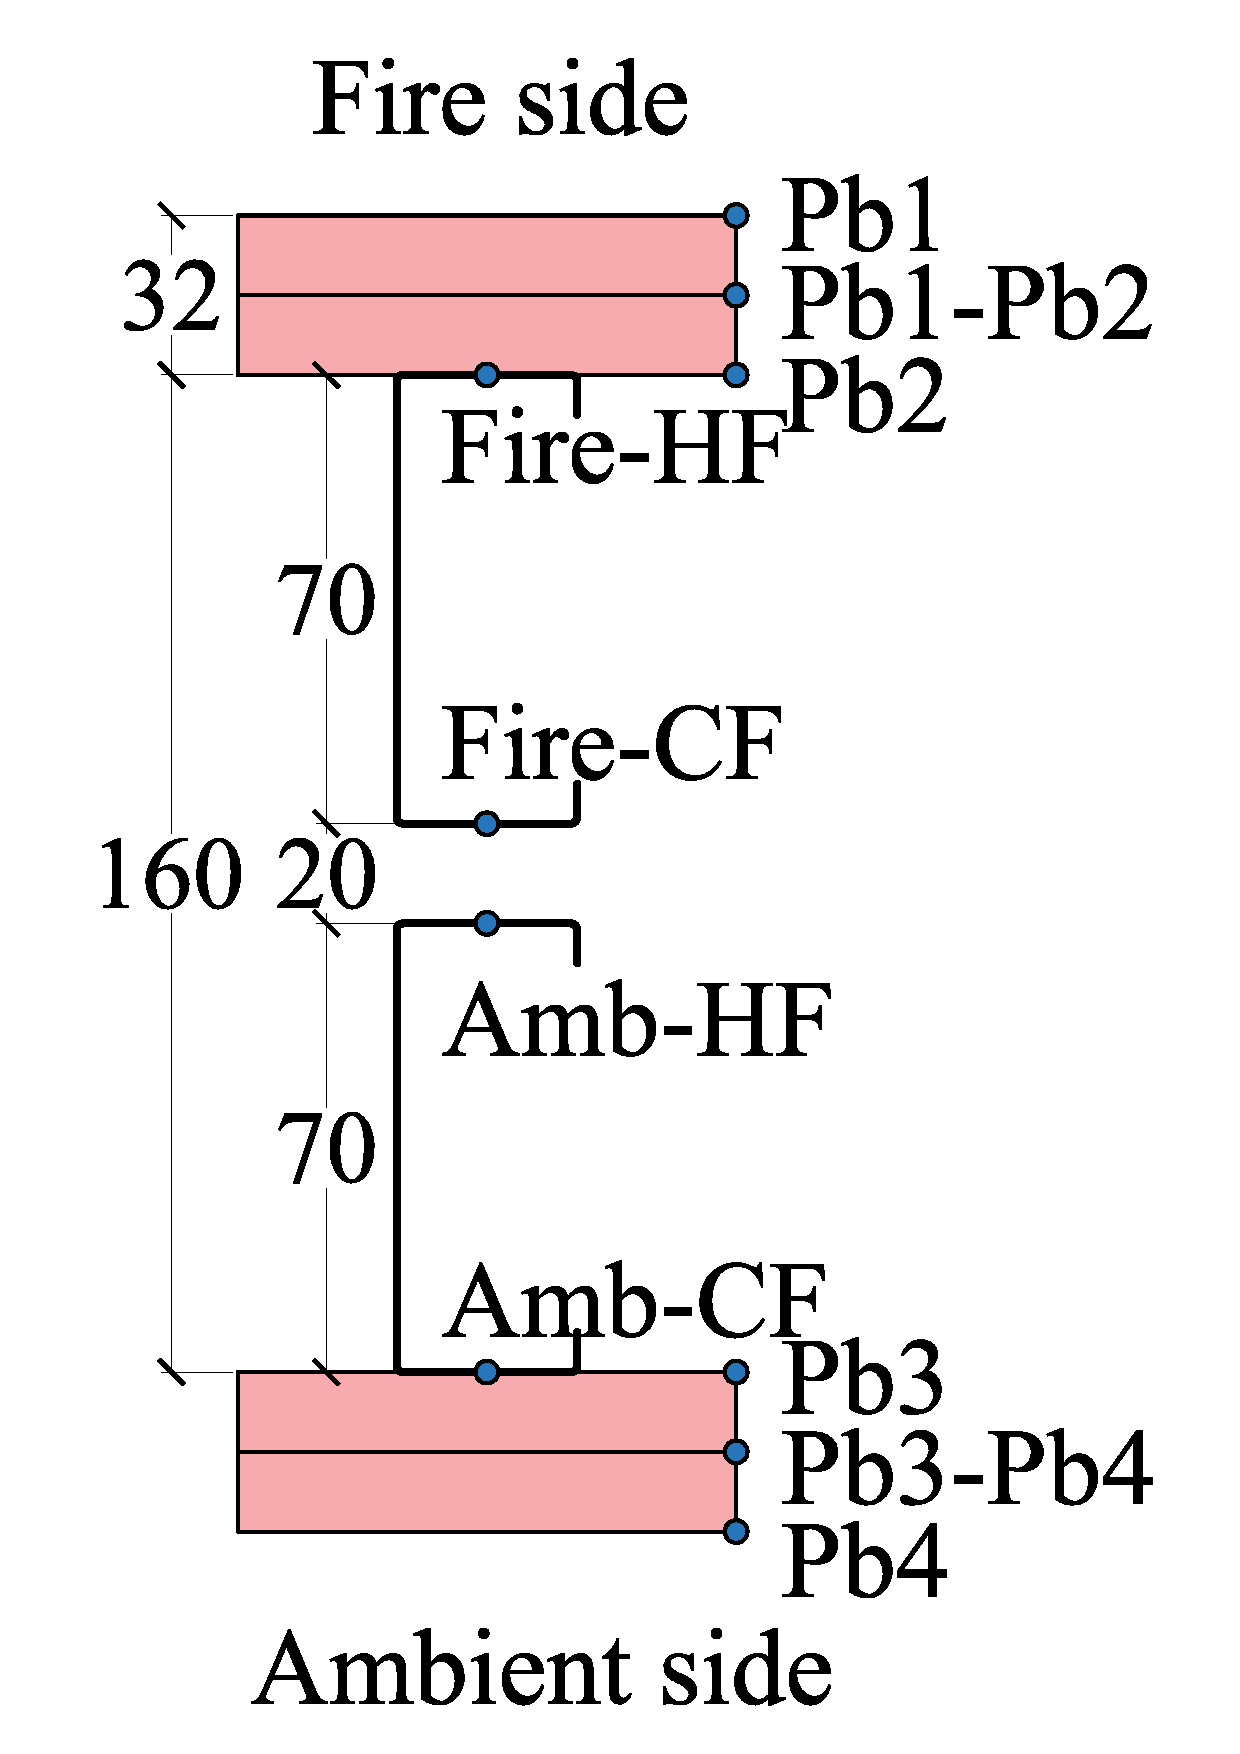
\includegraphics[width=\textwidth]{DS-70.pdf}
		\caption{}
		\label{subfig:DS-70}
	\end{subfigure}
	\begin{subfigure}[b]{0.2\textwidth}
		\centering
		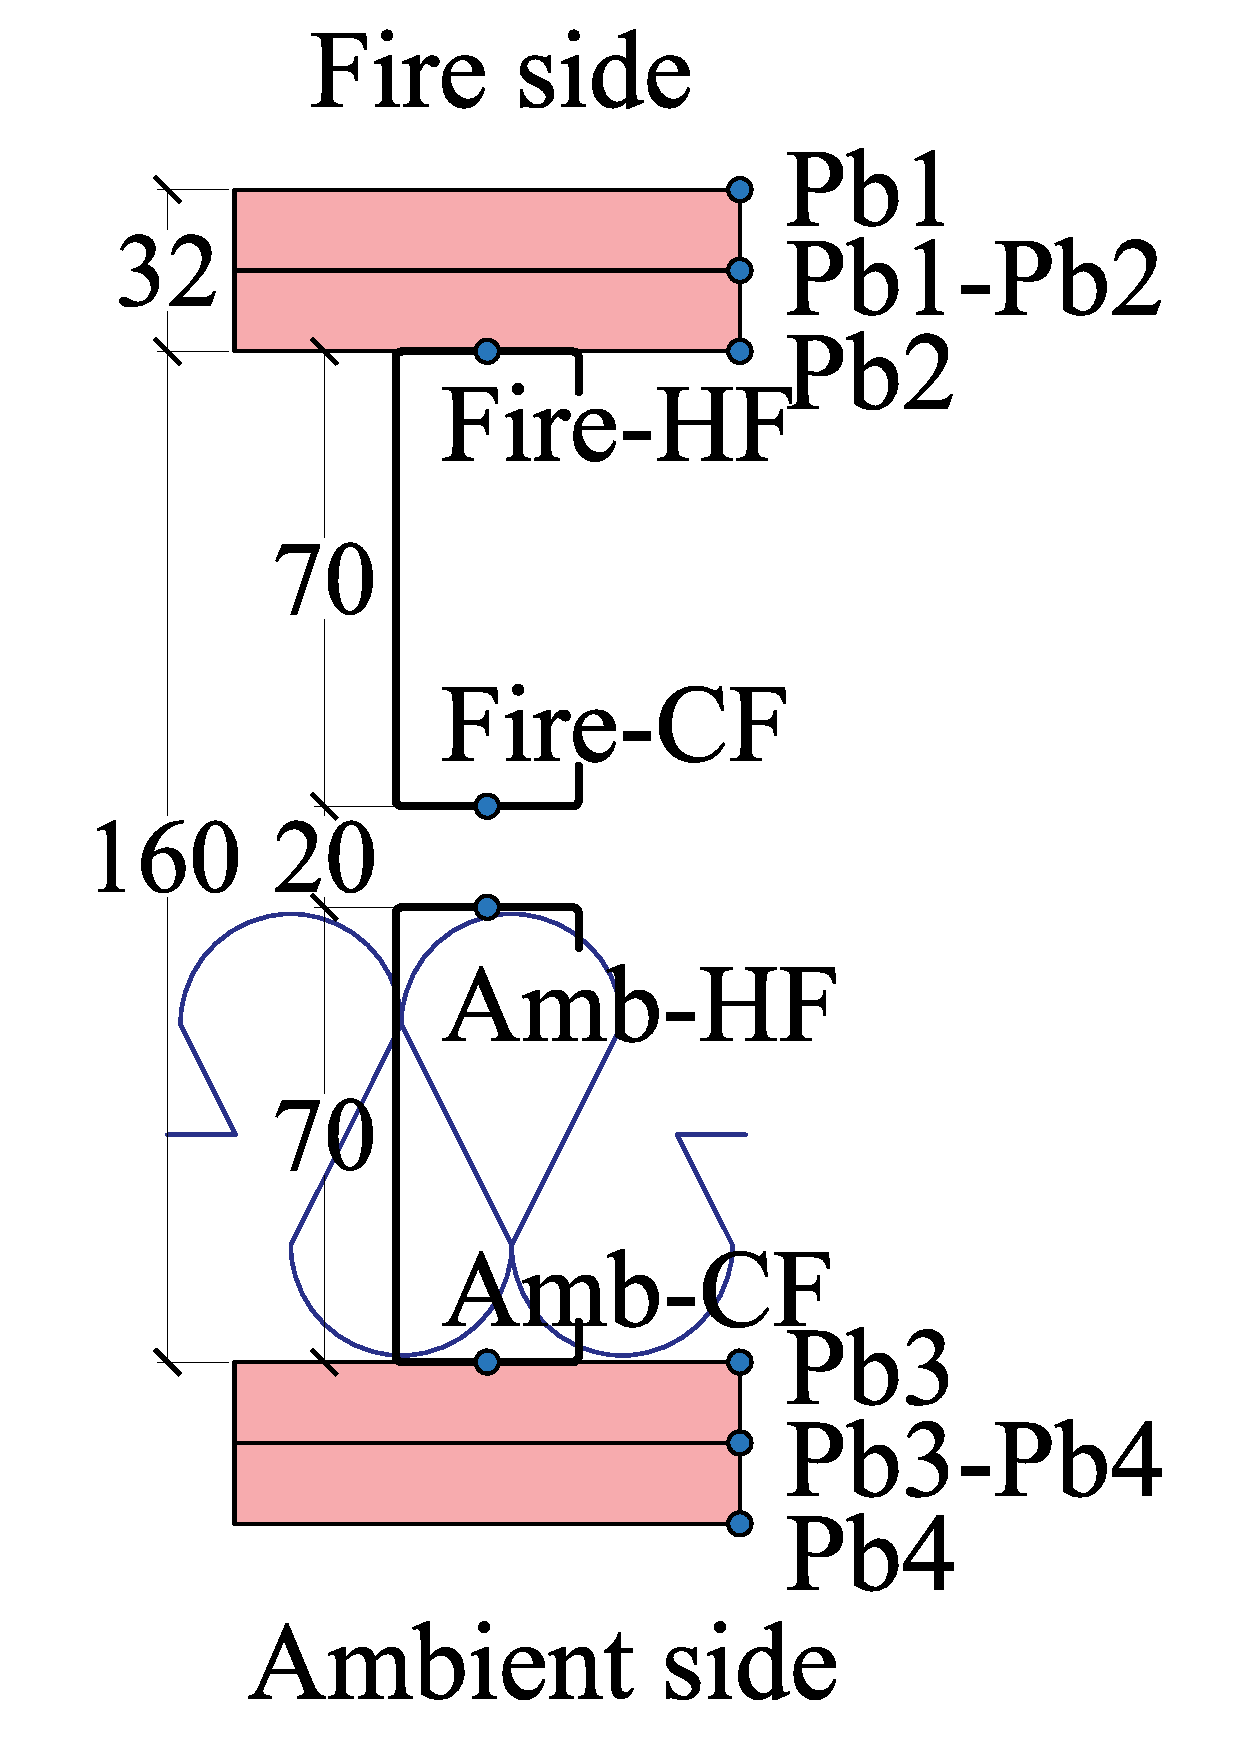
\includegraphics[width=\textwidth]{DS-70-AI.pdf}
		\caption{}
		\label{subfig:DS-70-AI}
	\end{subfigure}
	\begin{subfigure}[b]{0.2\textwidth}
		\centering
		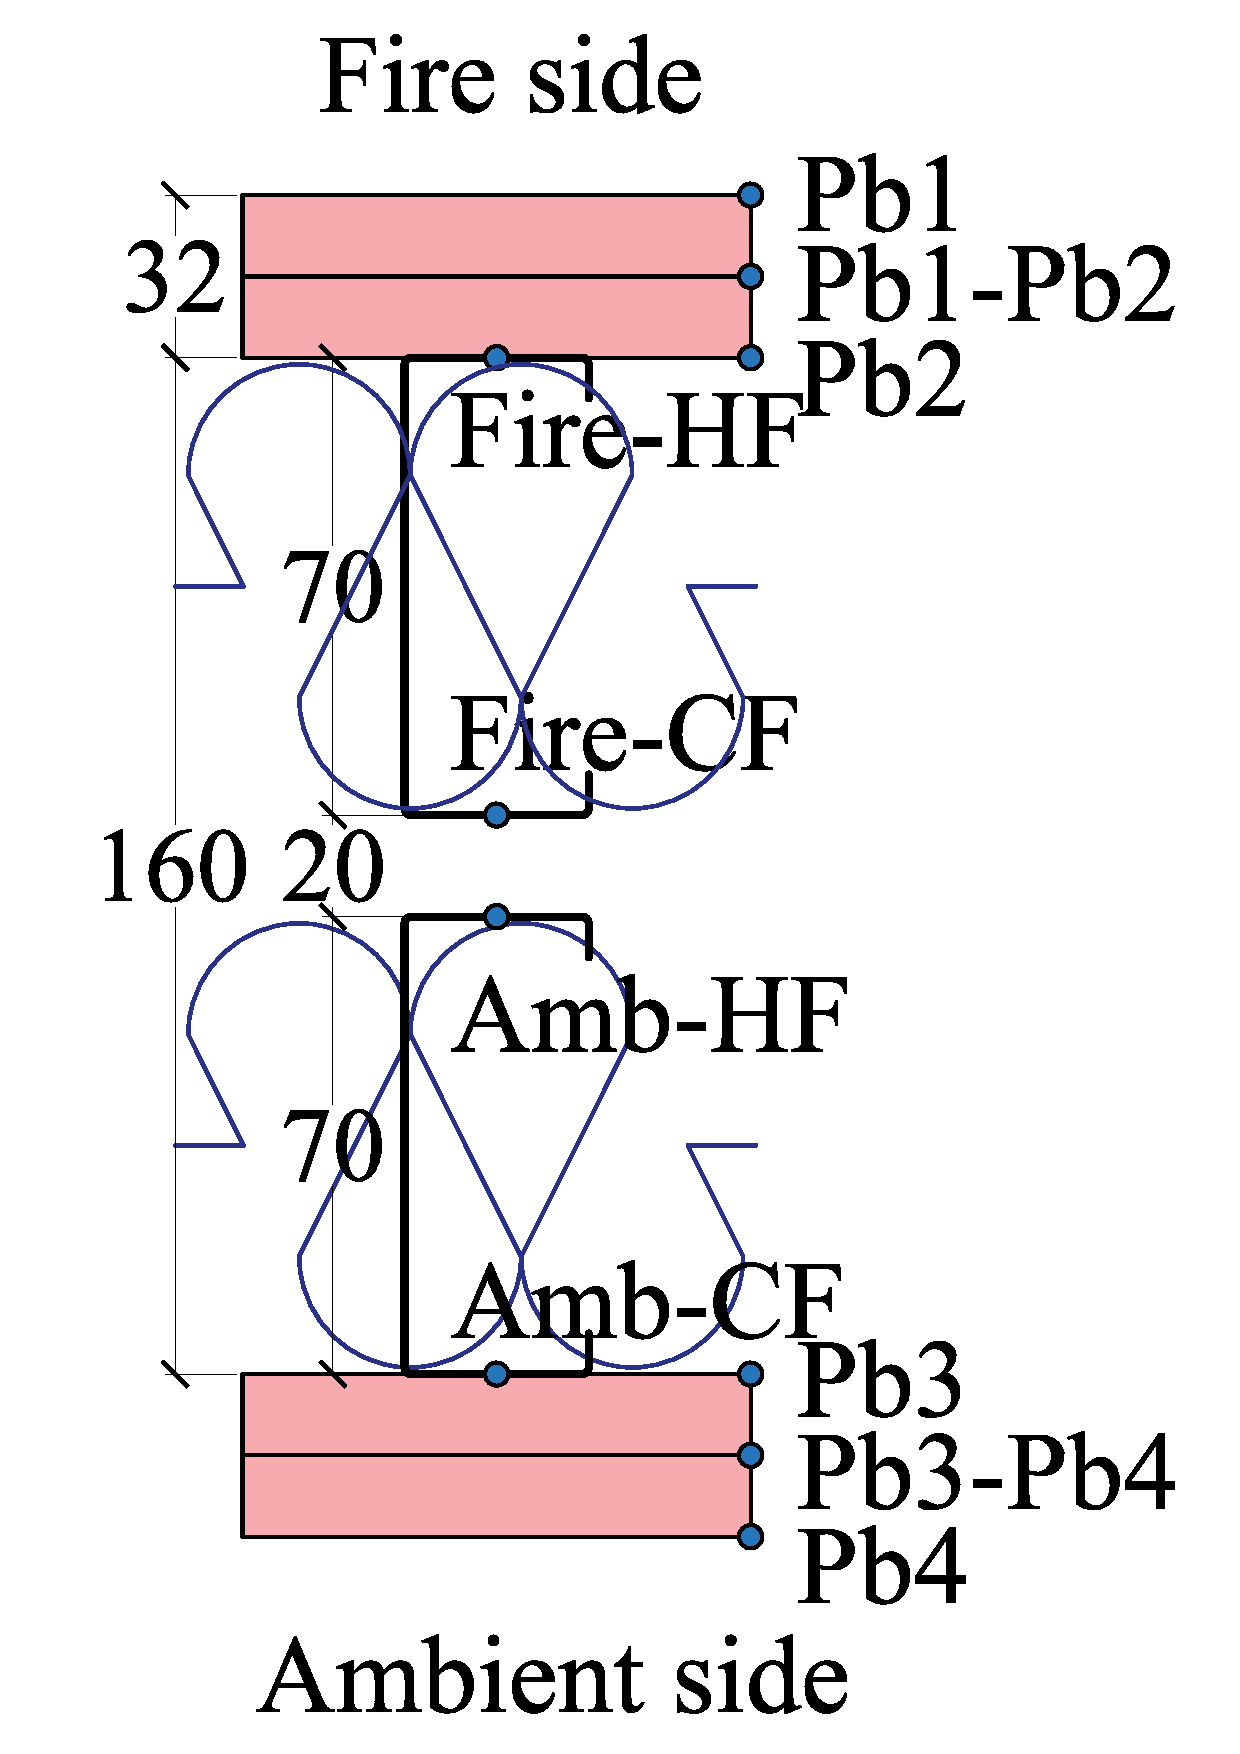
\includegraphics[width=\textwidth]{DS-70-BI.pdf}
		\caption{}
		\label{subfig:DS-70-BI}
	\end{subfigure}
	   \caption{Double Stud Wall with 70 mm studs (a) Non cavity insulated (b) Cavity insulation on the ambient side (c) Both cavity insulated}
	   \label{fig:DS-70-parametric}
\end{figure} 
\begin{figure}[!htbp]
	\centering
	\begin{subfigure}[b]{0.25\textwidth}
		\centering
		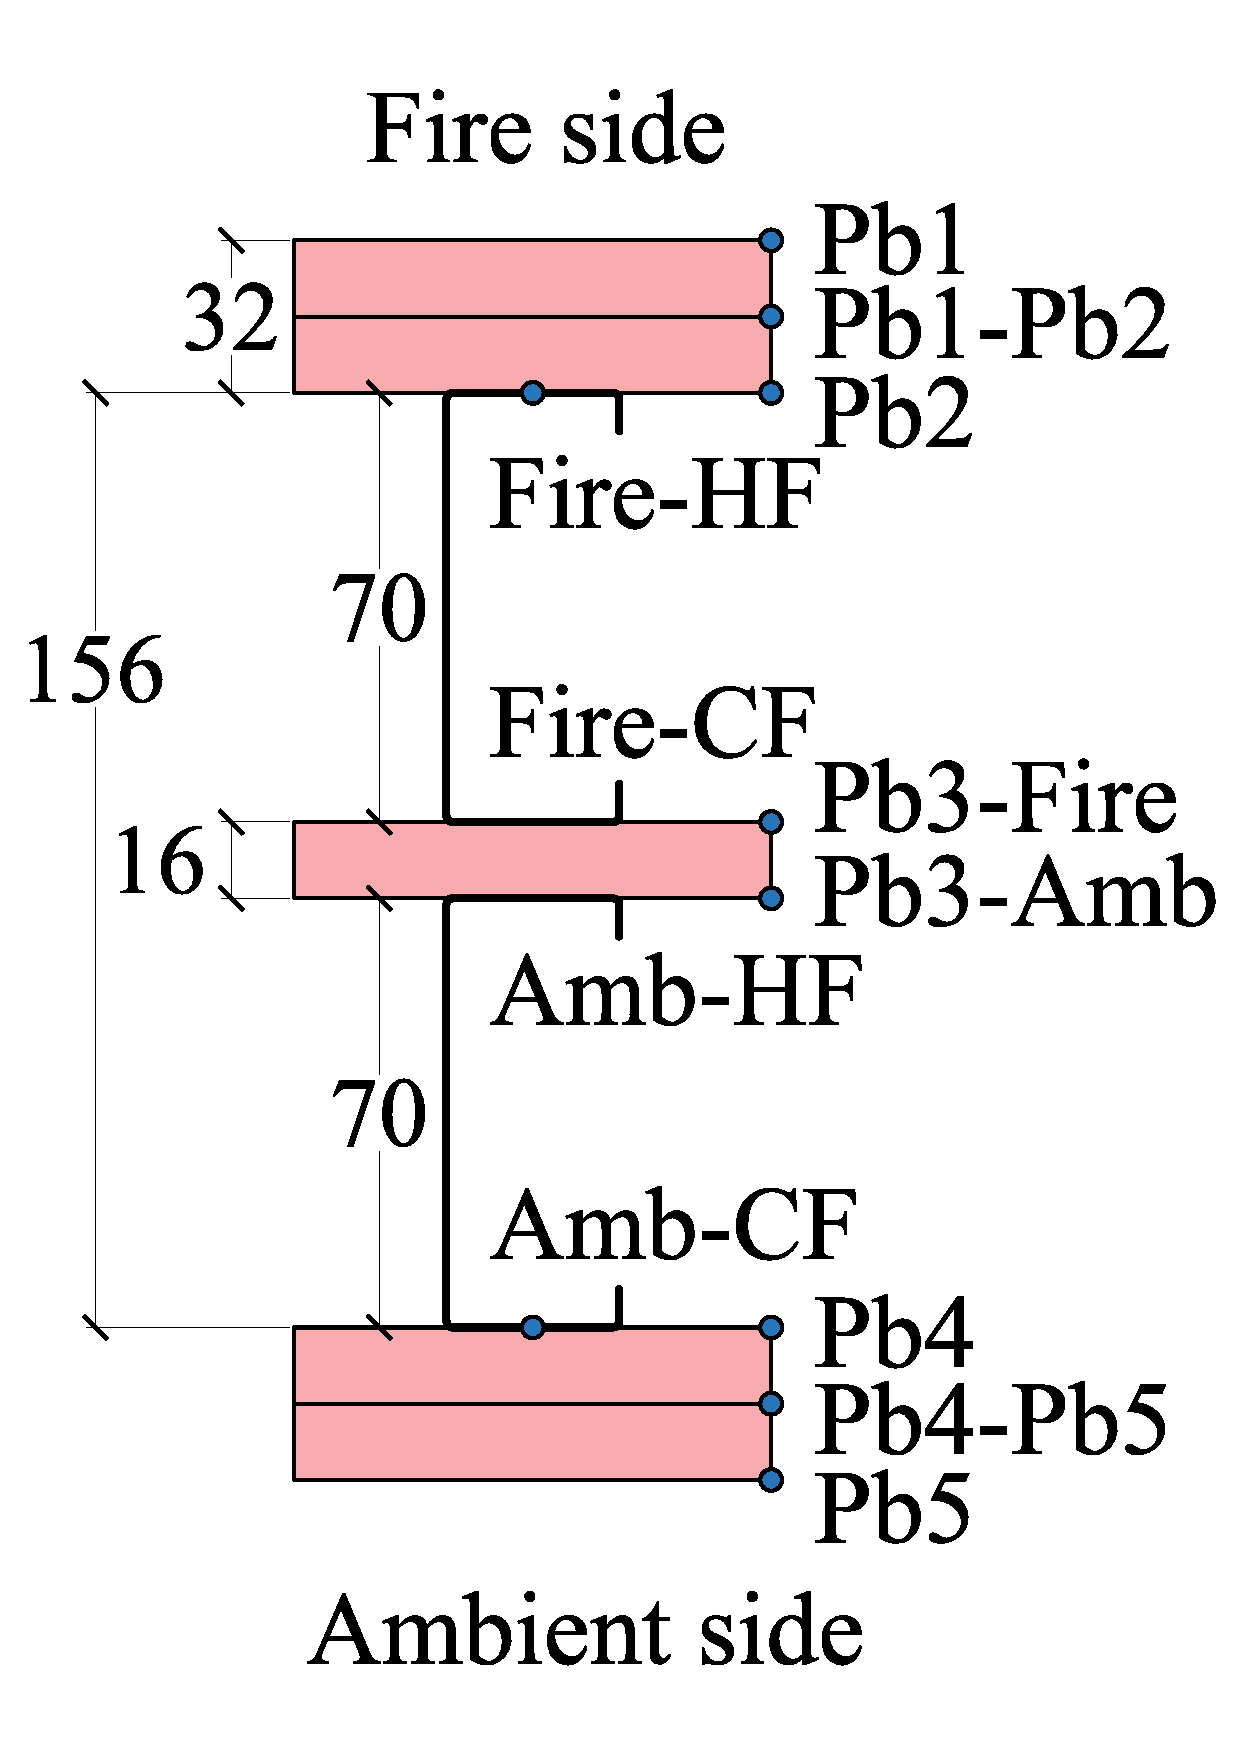
\includegraphics[width=\textwidth]{SL-70.pdf}
		\caption{}
		\label{subfig:SL-70}
	\end{subfigure}
	\begin{subfigure}[b]{0.25\textwidth}
		\centering
		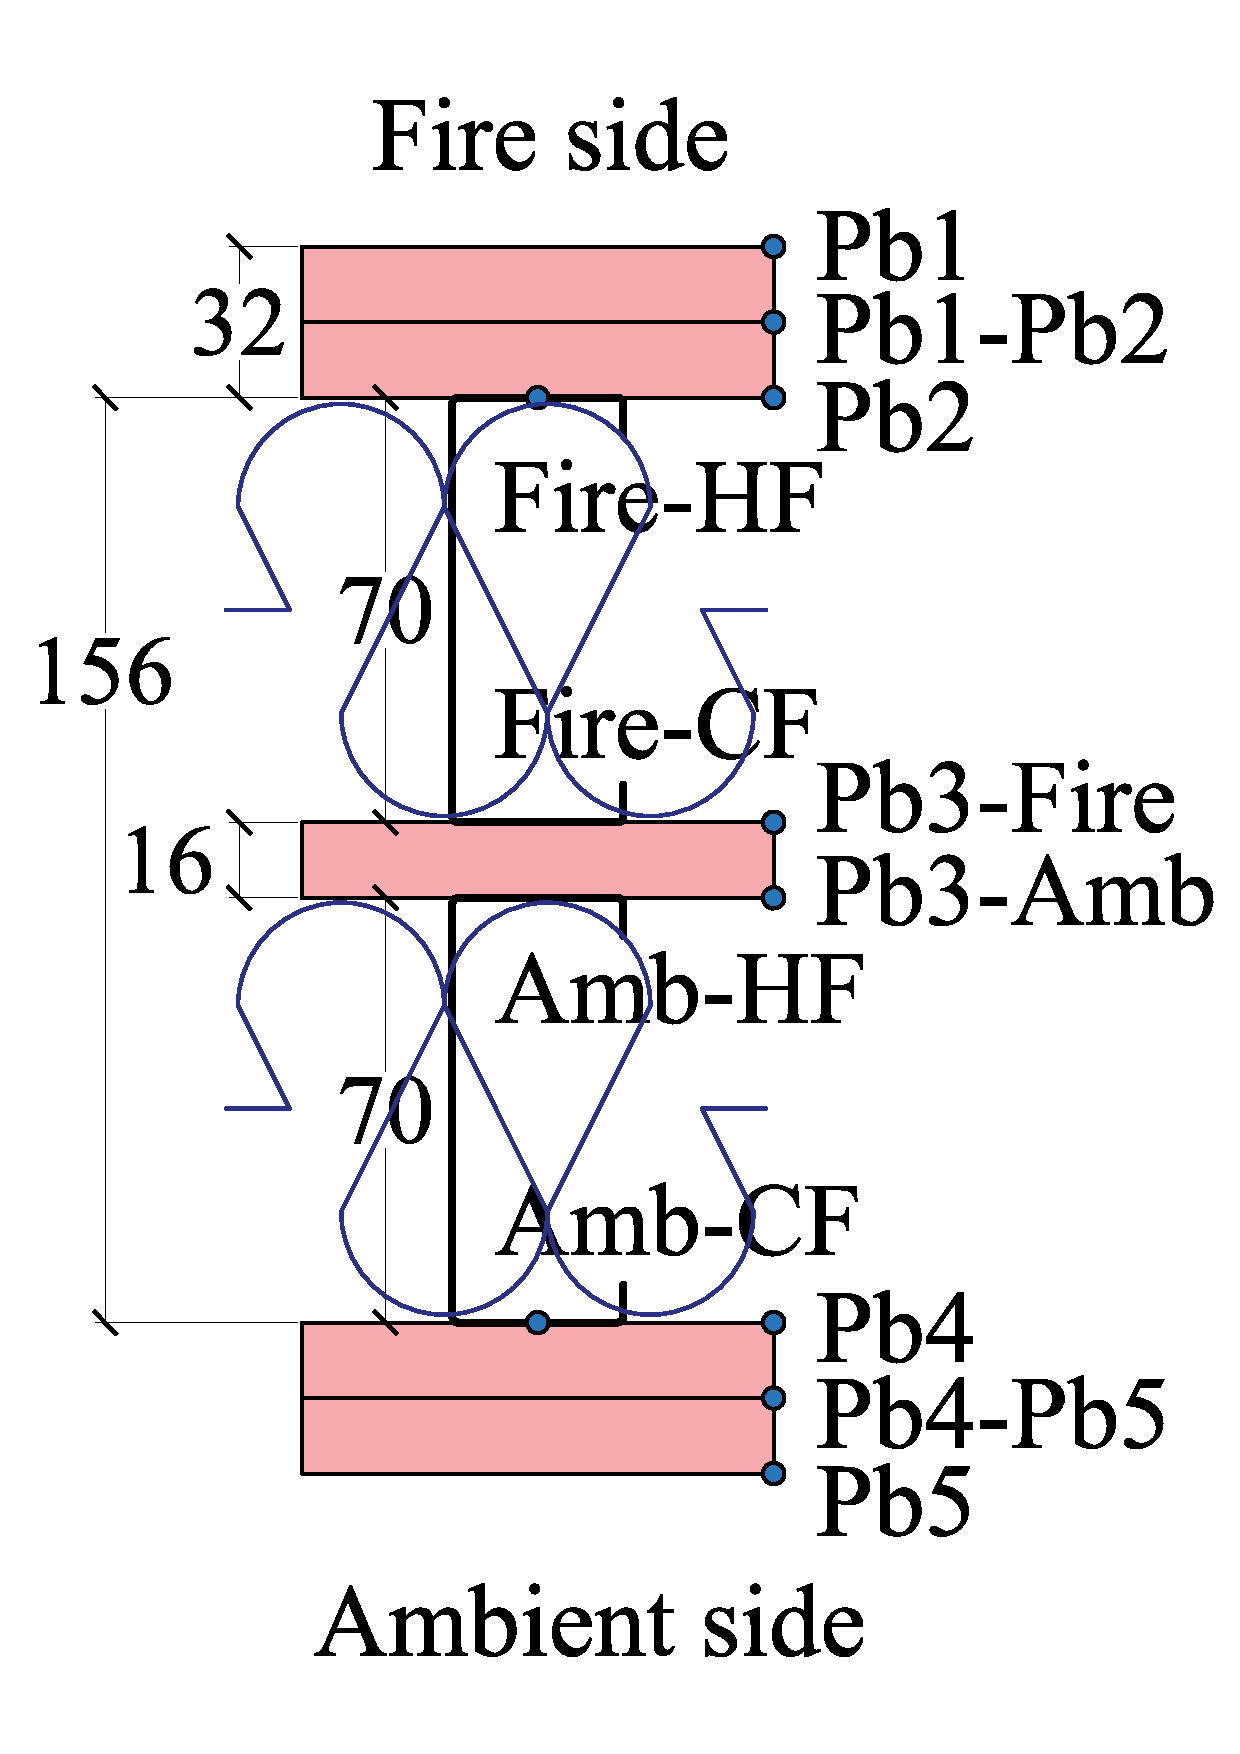
\includegraphics[width=\textwidth]{SL-70-BI.pdf}
		\caption{}
		\label{subfig:SL-70-BI}
	\end{subfigure}
	\begin{subfigure}[b]{0.25\textwidth}
		\centering
		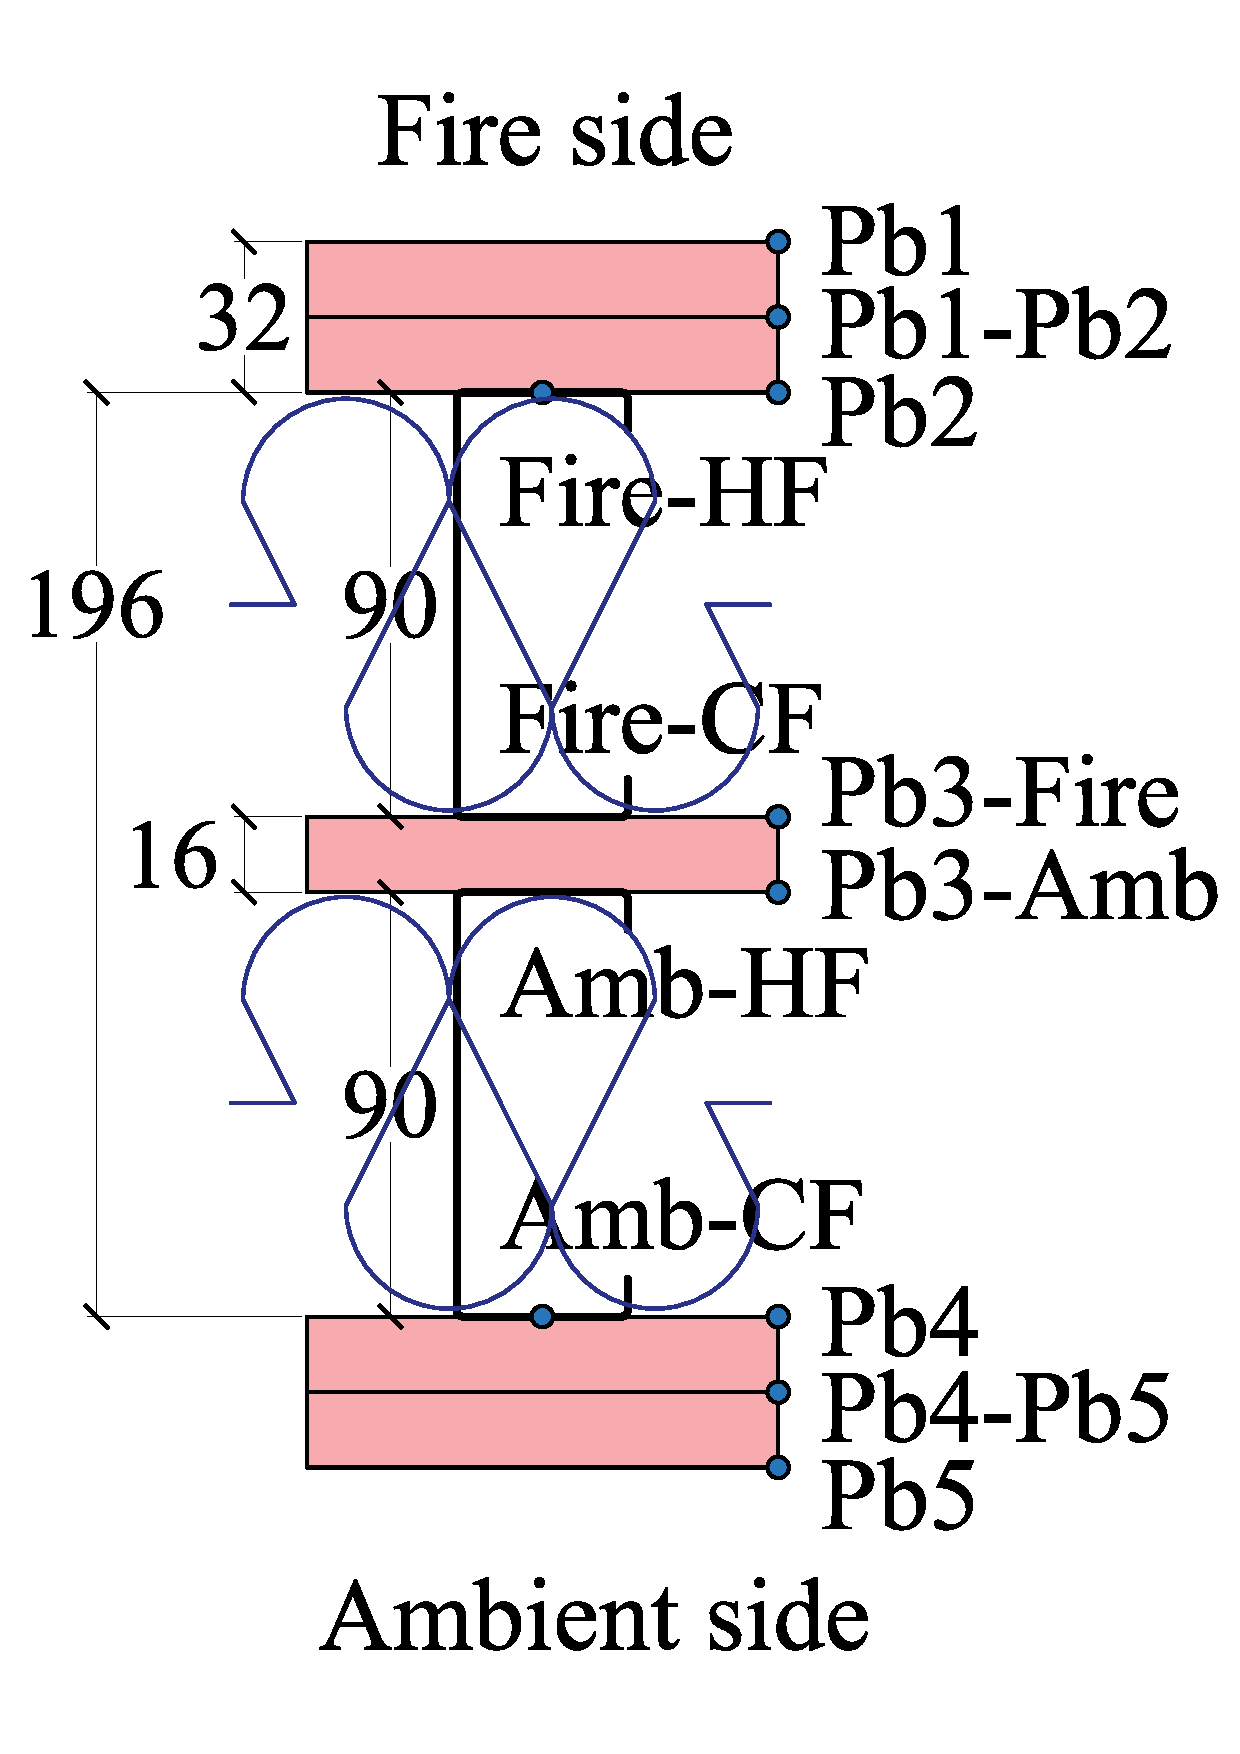
\includegraphics[width=\textwidth]{SL-90-BI.pdf}
		\caption{}
		\label{subfig:SL-90-BI}
	\end{subfigure}
	   \caption{Shaftliner Wall with 70 and 90 mm studs (a) Non cavity insulated 70 mm wall (b) Full cavity insulated 70 mm wall (c) Full cavity insulated 90 mm wall}
	   \label{fig:SL-70-90-parametric}
\end{figure} 
\begin{figure}[!htbp]
	\centering
	\begin{subfigure}[b]{0.35\textwidth}
		\centering
		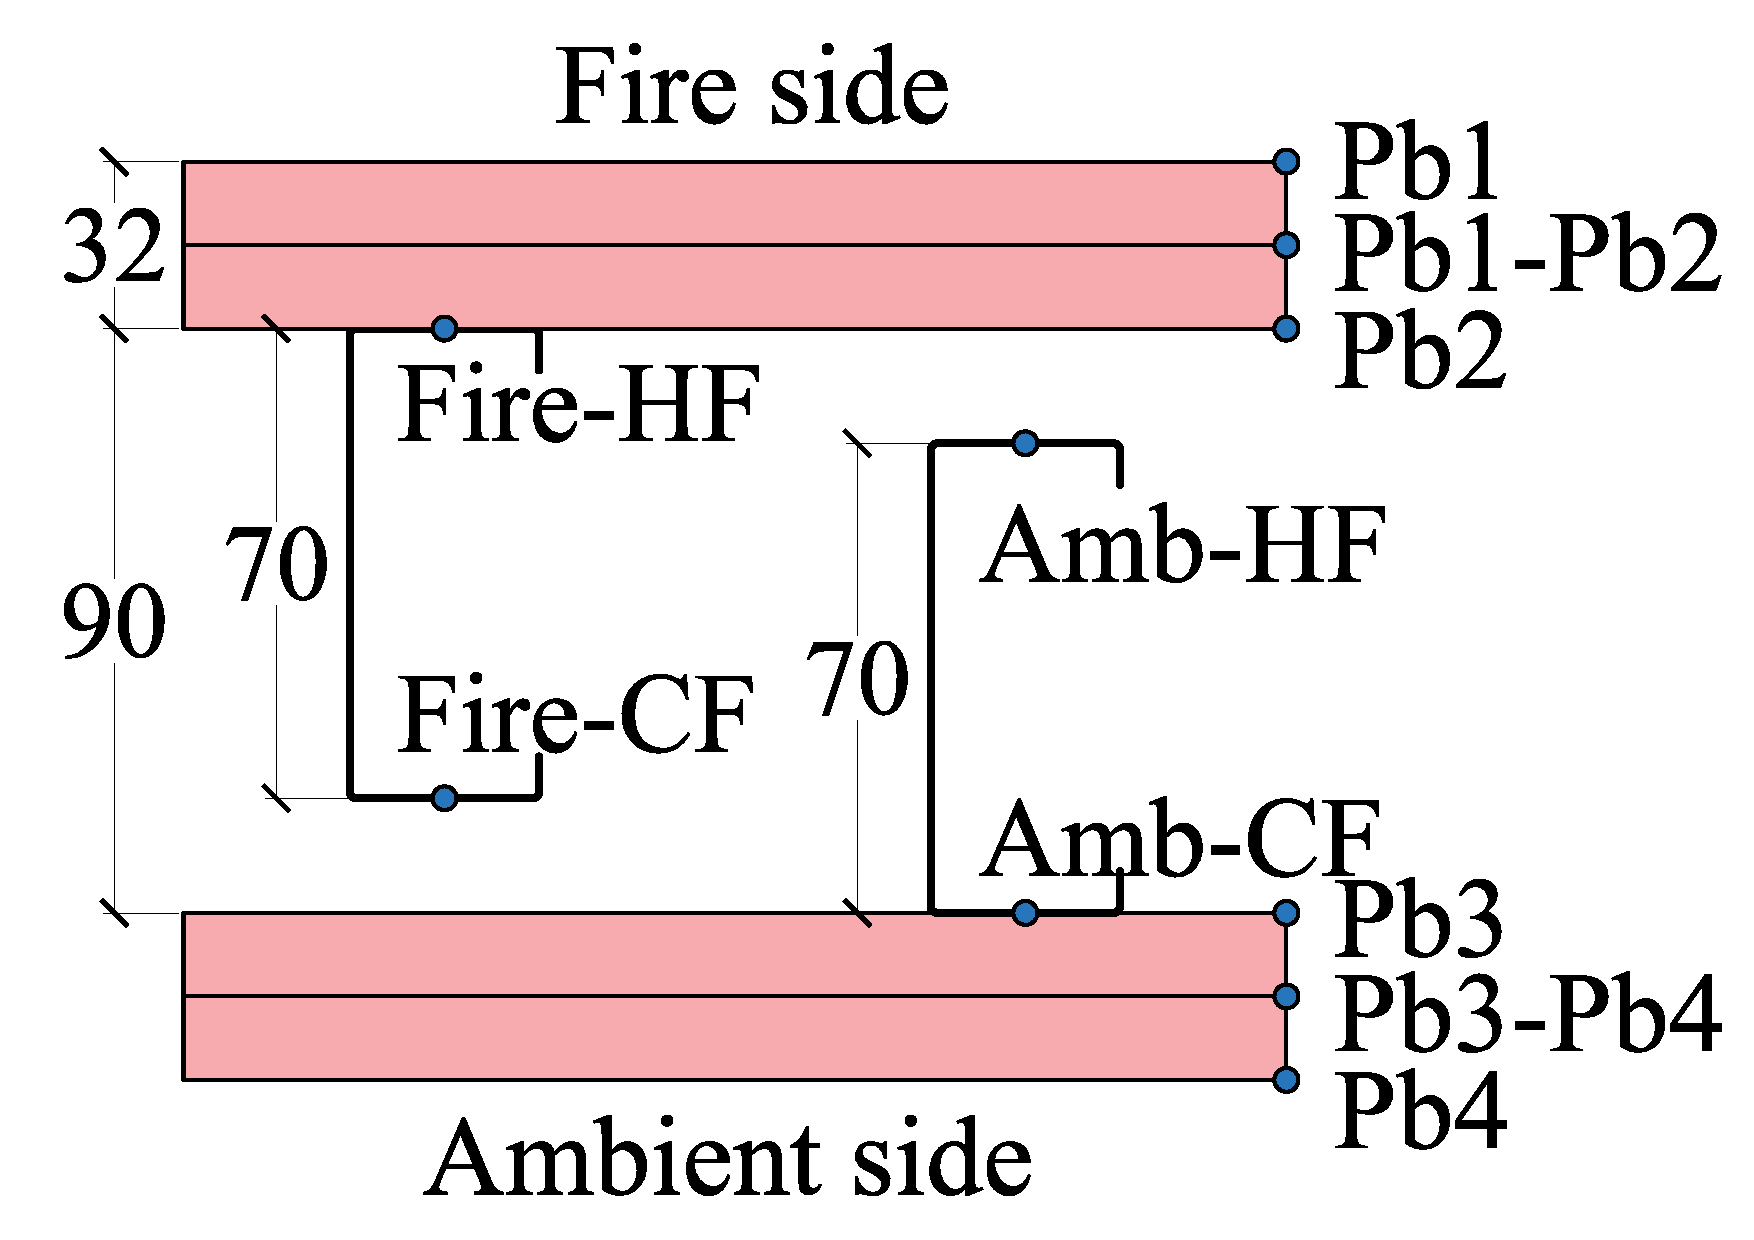
\includegraphics[width=\textwidth]{ST-70.pdf}
		\caption{}
		\label{subfig:ST-70}
	\end{subfigure}
	\begin{subfigure}[b]{0.35\textwidth}
		\centering
		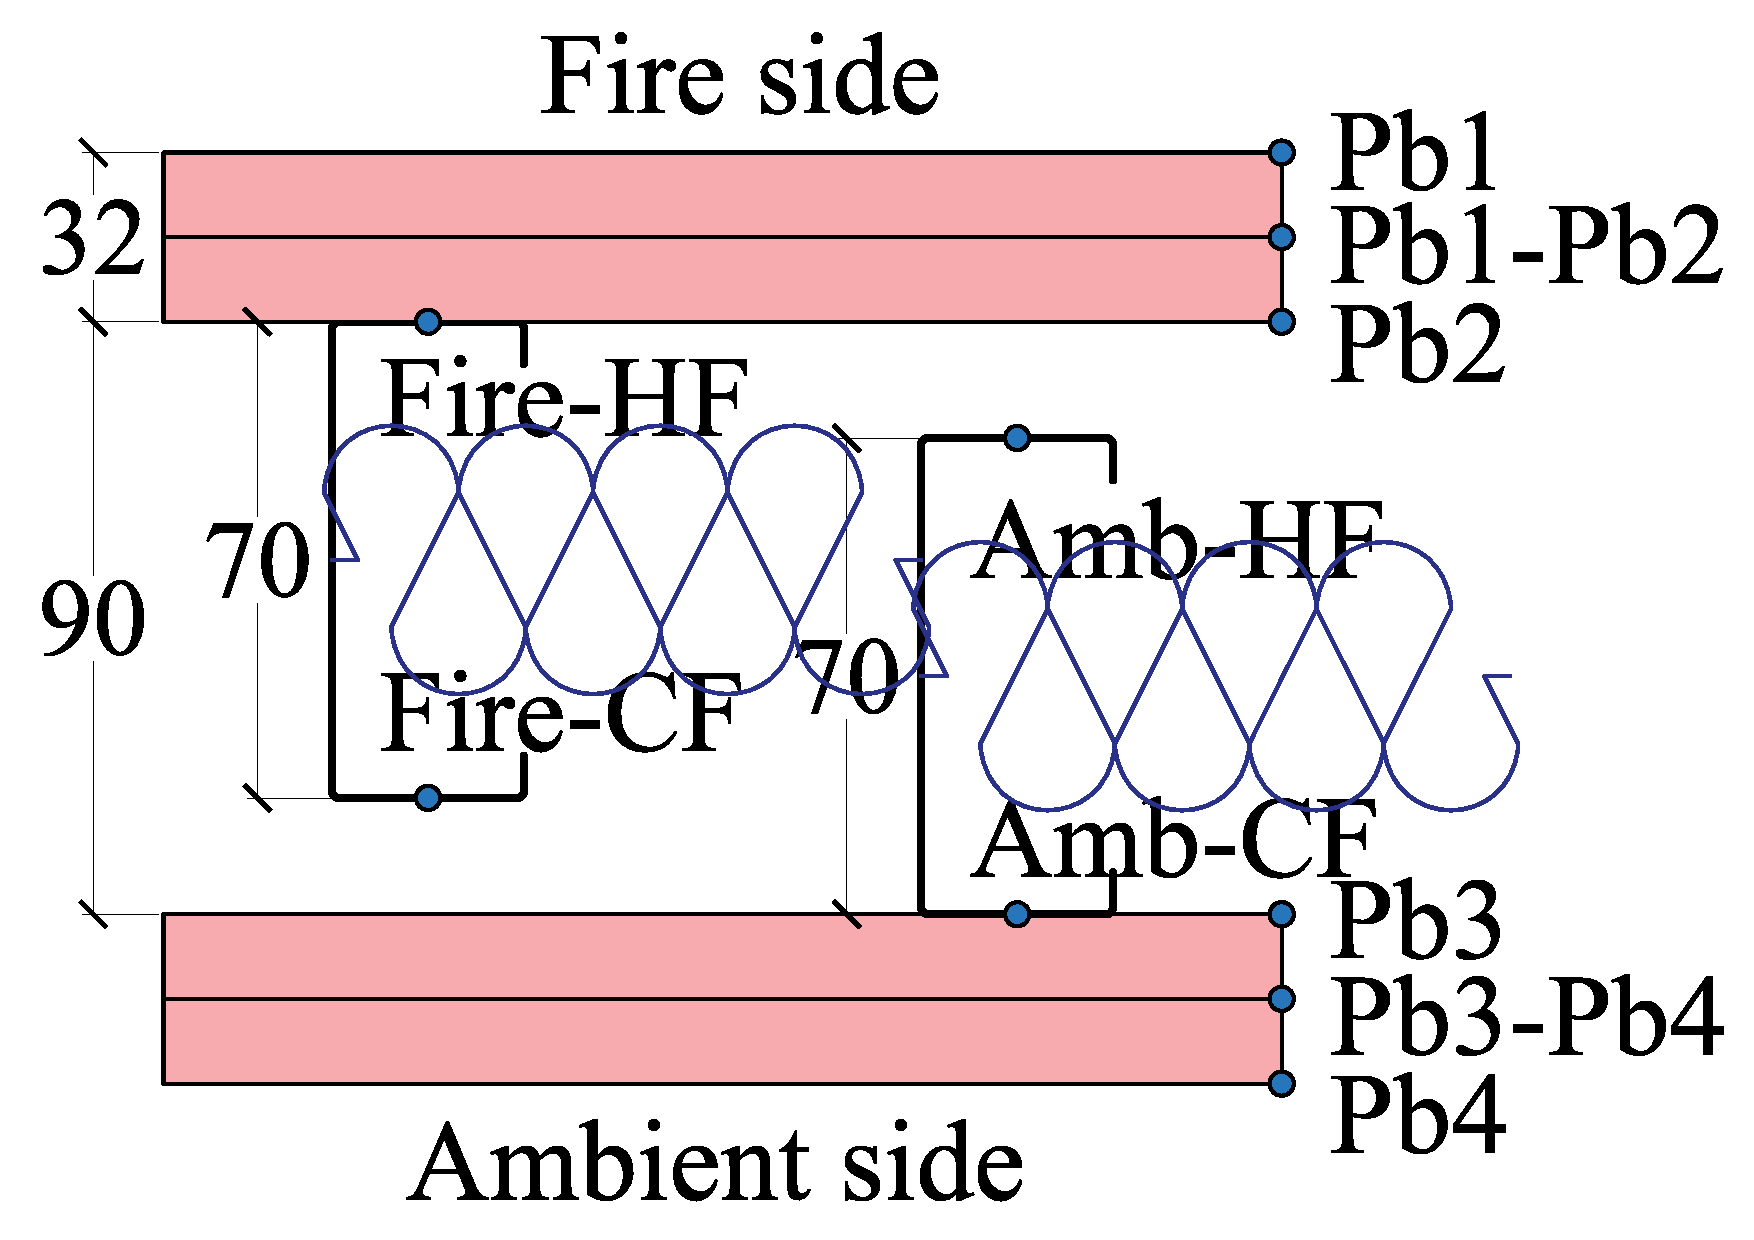
\includegraphics[width=\textwidth]{ST-70-FI.pdf}
		\caption{}
		\label{subfig:ST-70-FI}
	\end{subfigure}
	   \caption{Staggered Stud Wall with 70 mm studs (a) Non cavity insulated (b) Cavity insulated wall}
	   \label{fig:ST-70-parametric}
\end{figure} 
\begin{figure}[!htbp]
	\centering
	\begin{subfigure}[b]{0.35\textwidth}
		\centering
		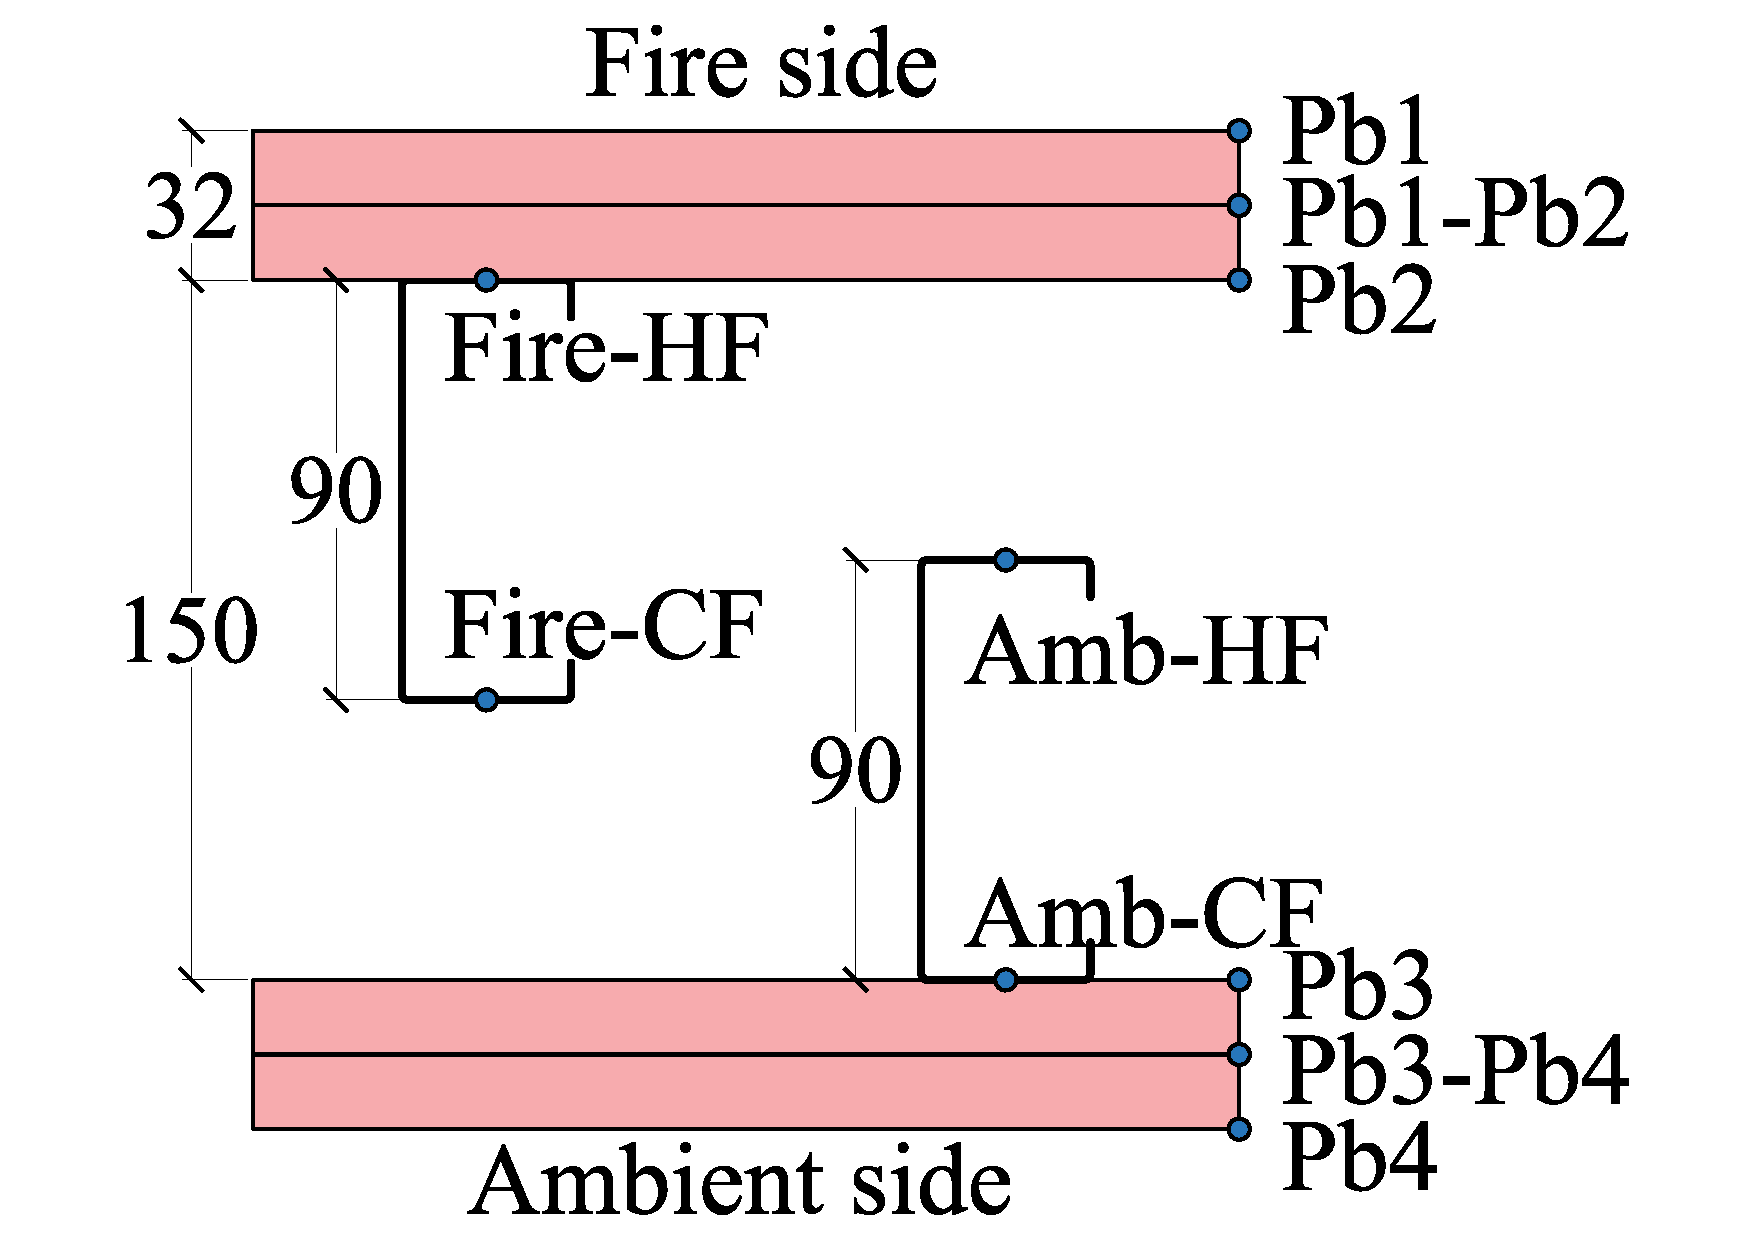
\includegraphics[width=\textwidth]{ST-90.pdf}
		\caption{}
		\label{subfig:ST-90}
	\end{subfigure}
	\begin{subfigure}[b]{0.35\textwidth}
		\centering
		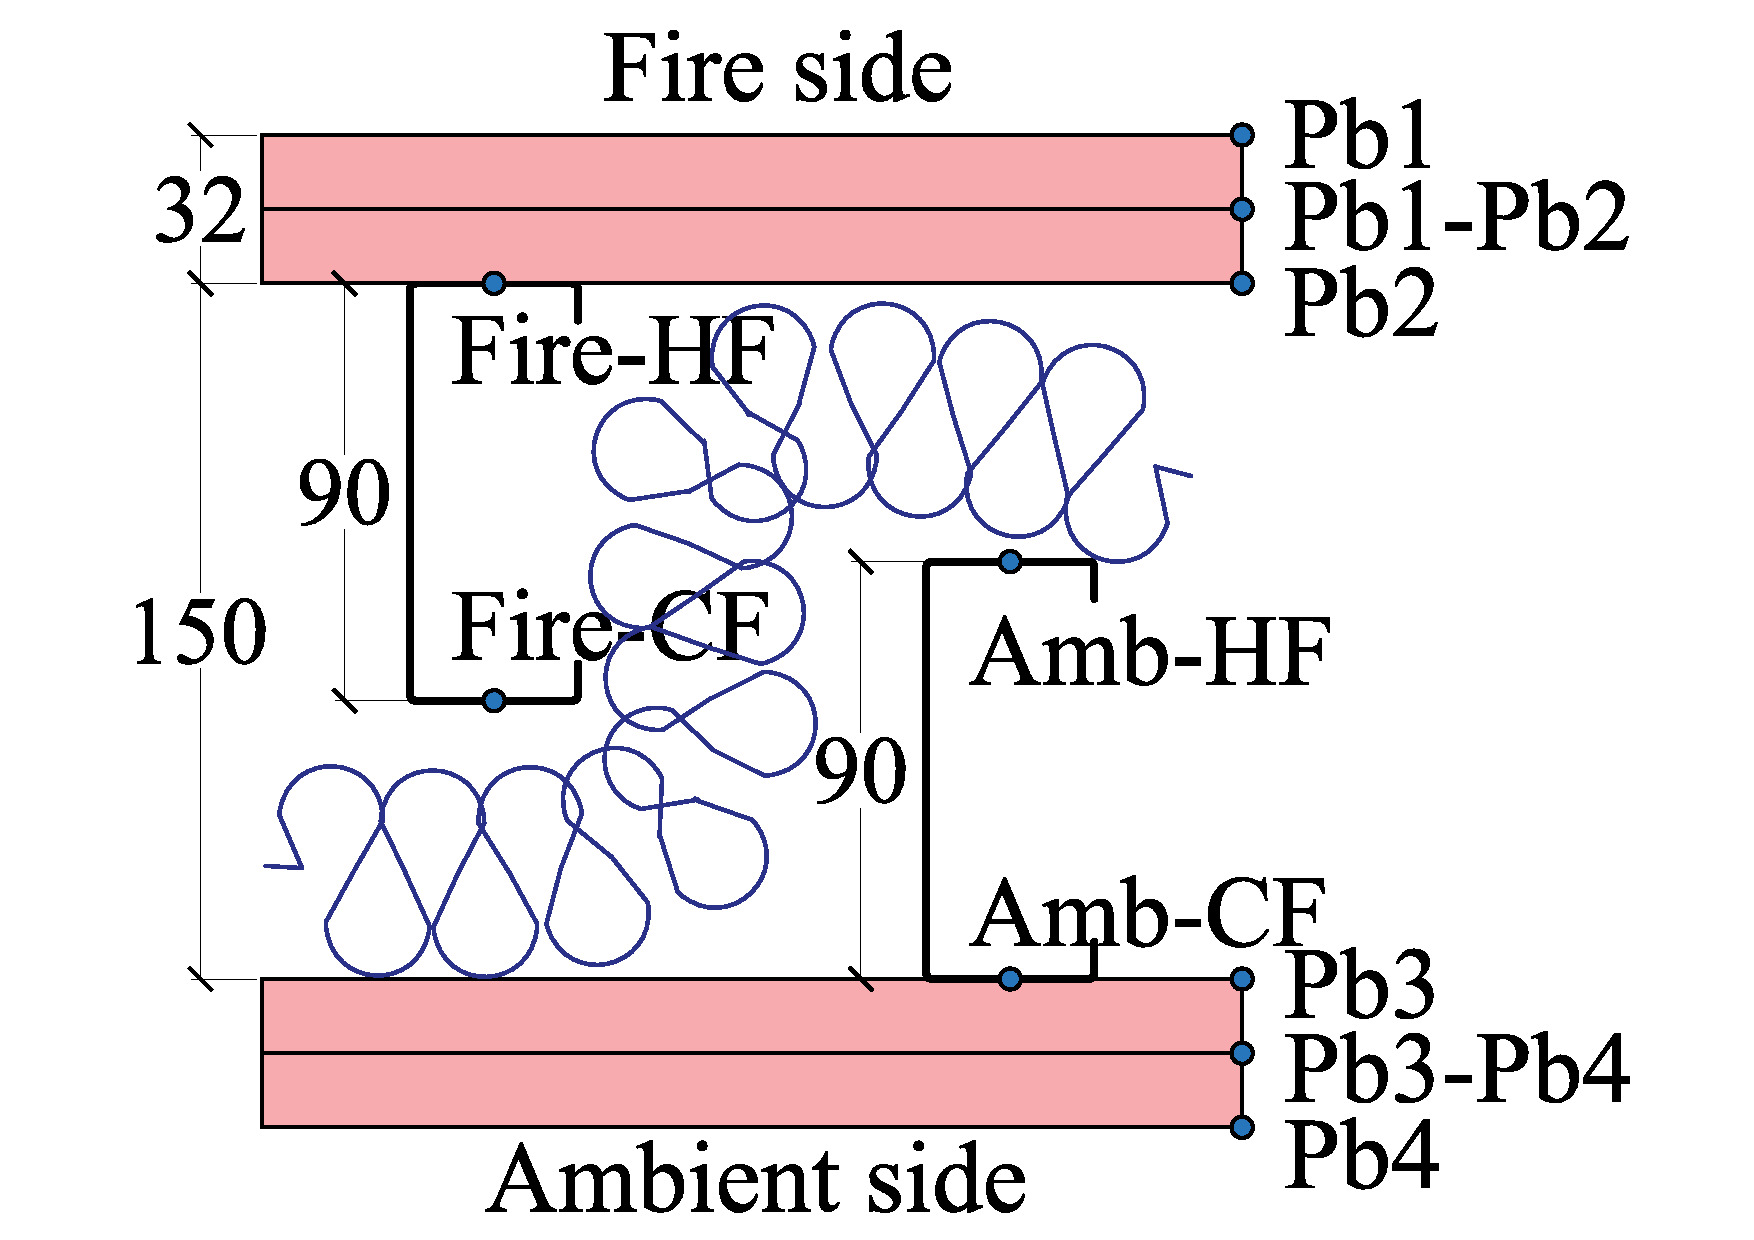
\includegraphics[width=\textwidth]{ST-90-FI.pdf}
		\caption{}
		\label{subfig:ST-90-FI}
	\end{subfigure}
	   \caption{Staggered Stud Wall with 70 mm studs (a) Non cavity insulated (b) Cavity insulated wall}
	   \label{fig:ST-90-parametric}
\end{figure} 

The LSF wall configurations considered for the parametric analysis are shown in \Cref{fig:DS-70-parametric,fig:SL-70-90-parametric,fig:ST-70-parametric}. \Cref{tab:fds-parametric-models} details the complex LSF wall configurations selected for the thermal parametric analysis. Some general notations will be followed to represent the models in the parametric study. DS represents Double stud wall, SL represents Shaftliner wall and ST represents Staggered stud wall with respect to the complex LSF wall configurations. AI represents ambient side cavity insulation, BI represents both cavity insulation and FI represents full cavity insulation.    
\begin{figure}[!htbp]
	\centering
	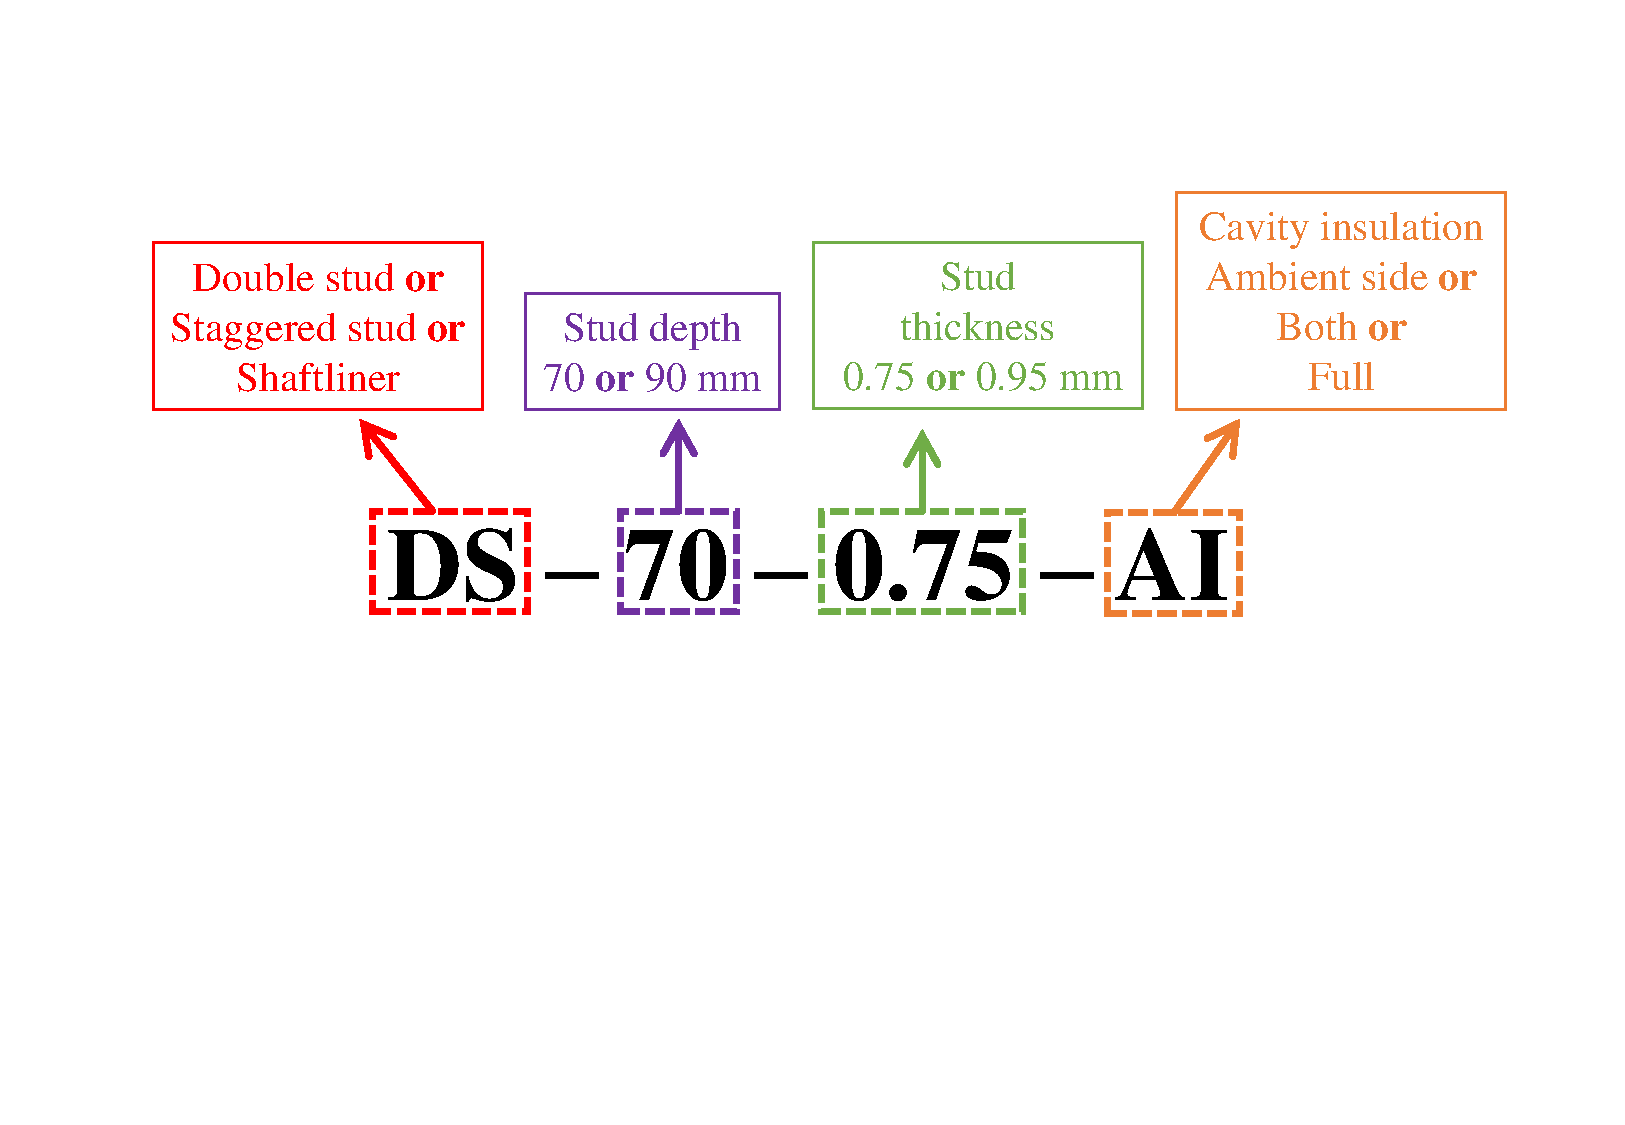
\includegraphics[scale=0.4]{parametric-notation.pdf}
	\caption{General notation for thermal parametric models}
	\label{parametric-notation}
\end{figure}
% Table generated by Excel2LaTeX from sheet 'Sheet3'
\begin{table}[htbp]
	\centering
	\caption{FDS Thermal models considered for parametric study}
	  \begin{tabular}{ccccc}
	  \toprule
	  \textbf{Model Name} & \textbf{Wall Type} & \textbf{Stud Depth} & \textbf{Stud Thickness} & \textbf{Insulation} \\
	  \midrule
	  DS-70-0.75 & \multirow{5}[2]{*}{Double stud} & \multirow{5}[2]{*}{70} & 0.75  & Nil \\
	  DS-70-0.75-AI &       &       & 0.75  & Ambient \\
	  DS-70-0.75-BI &       &       & 0.75  & Both \\
	  DS-70-0.95-AI &       &       & 0.95  & Ambient \\
	  DS-70-0.95-BI &       &       & 0.95  & Both \\
	  \midrule
	  DS-90-0.75-AI & \multirow{2}[2]{*}{Double stud} & \multirow{2}[2]{*}{90} & 0.75  & Ambient \\
	  DS-90-0.75-BI &       &       & 0.75  & Both \\
	  \midrule
	  SL-70-0.75 & \multirow{7}[4]{*}{Shaftliner} & \multirow{4}[2]{*}{70} & 0.75  & Nil \\
	  SL-70-0.75-FI &       &       & 0.75  & Full \\
	  SL-70-0.95 &       &       & 0.95  & Nil \\
	  SL-70-0.95-FI &       &       & 0.95  & Full \\
  \cmidrule{1-1}\cmidrule{3-5}    SL-90-0.75-FI &       & \multirow{3}[2]{*}{90} & 0.75  & Full \\
	  SL-90-0.95 &       &       & 0.95  & Nil \\
	  SL-90-0.95-FI &       &       & 0.95  & Full \\
	  \midrule
	  ST-70-0.75 & \multirow{6}[4]{*}{Staggered stud} & \multirow{4}[2]{*}{70} & 0.75  & Nil \\
	  ST-70-0.75-FI &       &       & 0.75  & Full \\
	  ST-70-0.95 &       &       & 0.95  & Nil \\
	  ST-70-0.95-FI &       &       & 0.95  & Full \\
  \cmidrule{1-1}\cmidrule{3-5}    ST-90-0.75 &       & \multirow{2}[2]{*}{90} & 0.75  & Nil \\
	  ST-90-0.75-FI &       &       & 0.75  & Full \\
	  \bottomrule
	  \end{tabular}%
	\label{tab:fds-parametric-models}%
  \end{table}%
  
\section{Thermal Parametric Models}\label{sec:thermal-parametric-models}

This section details the thermal parametric analysis conducted on the selected complex LSF wall configurations detailed in \Cref{tab:fds-parametric-models}. The time-temperature curves of plasterboards and studs were extracted from the FDS thermal analysis output and corresponding discussions are made. Considering the repetitive nature of the problem statement, snippets were created using PYTHON programming language for data extraction and plotting of the time-temperature curves from the FDS thermal analysis output. All the thermal models were analysed under two conditions. Firstly the model was analysed without considering plasterboard open-up. Then plasterboard open-up was accounted based on the ''SETPOINT" temperature depending on the LSF wall configuration which was classified into non-cavity insulated and cavity insulated walls. In general construction practices, LSF wall configurations can be used under load bearing and non-load bearing conditions. Therefore, predicting the thermal behaviour under load bearing and non-load bearing conditions will yield better understanding on the thermal performance of these complex LSF walls. Some general notations along with those previously mentioned will be followed to represent the time-temperature curve of the models with and without plasterboard open-up. "Fds-O" represents the time-temperature curves with plasterboard open-up while ''Fds" in the legend represents time-temperature curve corresponding to model without plasterboard open-up.

\subsection{Double stud wall with 70 mm studs}\label{sec:ds-70-thermal-fds}

FDS thermal analysis conducted on 70 mm double stud walls with and without cavity insulation are discussed in this section. \Cref{fig:DS-70-075-2x16-r3} shows the time-temperature curves from FDS thermal analysis conducted on non-cavity insulated double stud LSF walls with 70 $\times$ 0.75 mm studs (DS-70-0.75 as shown in \Cref{subfig:DS-70}). The effective cavity depth in the considered model was 160 mm (70$\times$2$+$20$=$160). The fire side plasterboard time-temperature curve (Fds-Pb1) exhibited reasonable agreement with the input ISO 834 standard time-temperature curve as shown in \Cref{subfig:DS-70-075-2x16-r3-PB}. A small dip in the Fds-O-Pb1 time-temperature curve is noticeable at 175 min. However, this was not observed in the Fds-Pb1 time-temperature curve. This is a resultant of the plasterboard open-up simulated in the FDS thermal model. The fire side plasterboard interface Fds-O-Pb1-Pb2 exhibited a steady increase in the time-temperature curve till 120 min of the simulation after which the curve tends to exhibit a plateau. However, the fire side cavity (Fds-O-Pb2) time-temperature curve recorded temperatures significantly less than the fire side interface (Pb1-Pb2). The sudden increase in the Fds-O-Pb2 curve at 175 min confirms the plasterboard open-up. But the Fds-Pb2 continues till the end of simulation by exhibiting a gradual increase. Similar trend is followed by the ambient side cavity (Fds-O-Pb3) time-temperature curve. The ambient side plasterboard interface (Fds-O-Pb3-Pb4) time-temperature curve recorded temperature less than 200\degree C till 220 min of simulation. Likewise, the ambient side plasterboard (Fds-Pb4) temperatures were less than 100\degree C till the end of simulation despite considering the plasterboard open-up. This infers the absence of insulation failure in the selected double stud wall configuration. The sudden increase in the time-temperature curves in the plasterboard open-up model is because the heat from the fire side is let into the cavity thereby exposing the studs and plasterboard directly to the input ISO 834 time-temperature curve.
\begin{figure}[!htbp]
	\centering
	\begin{subfigure}[b]{0.6\textwidth}
		\centering
		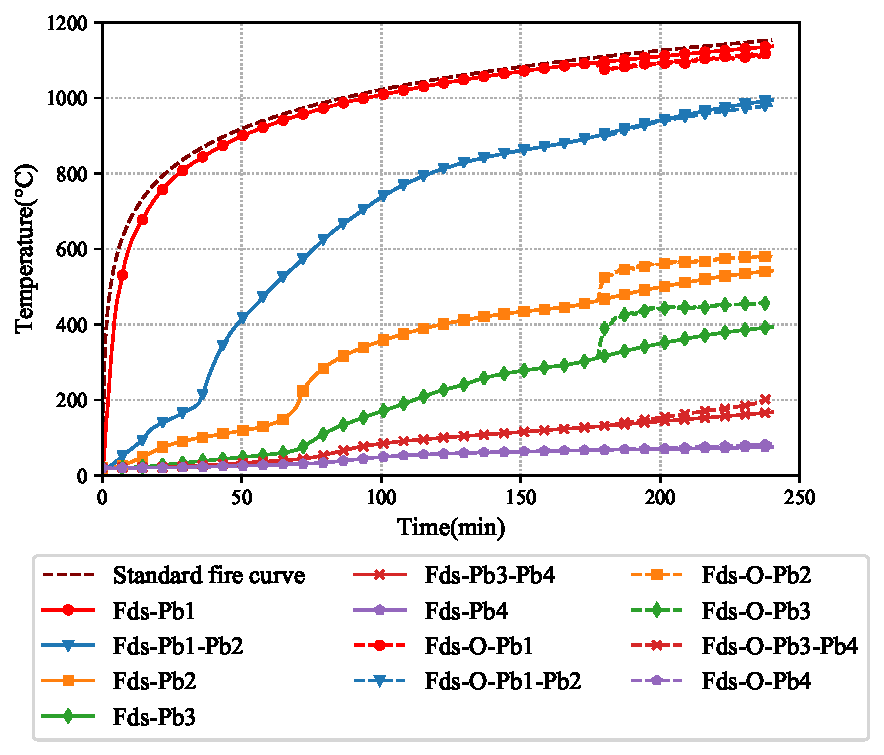
\includegraphics[width=\textwidth]{DS-70-075-2x16-r3-PB.pdf}
		\caption{}
		\label{subfig:DS-70-075-2x16-r3-PB}
	\end{subfigure}
	\begin{subfigure}[b]{0.6\textwidth}
		\centering
		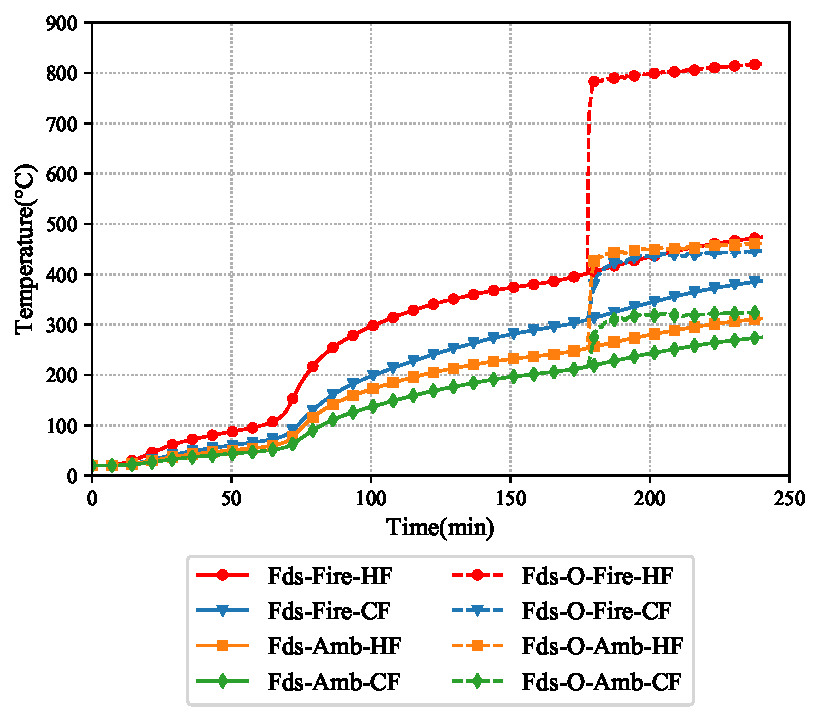
\includegraphics[width=\textwidth]{DS-70-075-2x16-r3-Studs.pdf}
		\caption{}
		\label{subfig:DS-70-075-2x16-r3-Studs}
	\end{subfigure}
	   \caption{Model DS-70-0.75 - Plasterboard and stud time-temperature curves of non-cavity insulated double stud wall with 70 $\times$ 0.75 mm studs - (a) Plasterboard temperatures (b) Stud temperatures}
	   \label{fig:DS-70-075-2x16-r3}
\end{figure} 

The stud hot and cold flange temperatures from the DS-70-0.75 model is shown in \Cref{subfig:DS-70-075-2x16-r3-Studs}. The stud fire side hot flange temperature Fds-O-Fire-HF showed a gradual increase till plasterboard open-up after which a sudden increase in the curve is noticed. This is reflected in the corresponding fire side cold flange (Fds-O-Fire-CF) and the ambient side hot and cold flanges (Fds-O-Amb-HF and CF). It is to note that the difference in the Fds-O-Fire-HF and CF time-temperature curve is minimal is the early stages of simulation and continues till the plasterboard open-up. This minimal difference in the time-temperature curve is also noticed on the Fds-O-Amb-HF and CF curves. However, post plasterboard open-up the difference in the hot and cold flange temperatures becomes large. This may be due to the fire side hot flange getting directly exposed to the input ISO 834 time-temperature curve. Also as the corresponding cold flange (Fds-O-Fire-CF) is separated by 20 mm gap there prevails no heat transfer through conduction similar to full-scale fire Test-T1 in \Cref{ch:Fire}. However, the difference between the other flanges apart from the Fds-O-Fire-HF is minimal. This is because of the non exposure of the other flanges to the ISO 834 time-temperature curve. Due to the absence of insulation within the cavity there is significant loss of heat from the stud surfaces into the cavity resulting this unique behaviour in the time-temperature curve. The steep increase during plasterboard open-up was not witnessed on the Fds-Fire-HF time-temperature curve. The maximum temperature achieved by the model with plasterboard open-up was 829\degree C while it was 497\degree C for the model without plasterboard open-up. 
\begin{figure}[!htbp]
	\centering
	\begin{subfigure}[b]{0.6\textwidth}
		\centering
		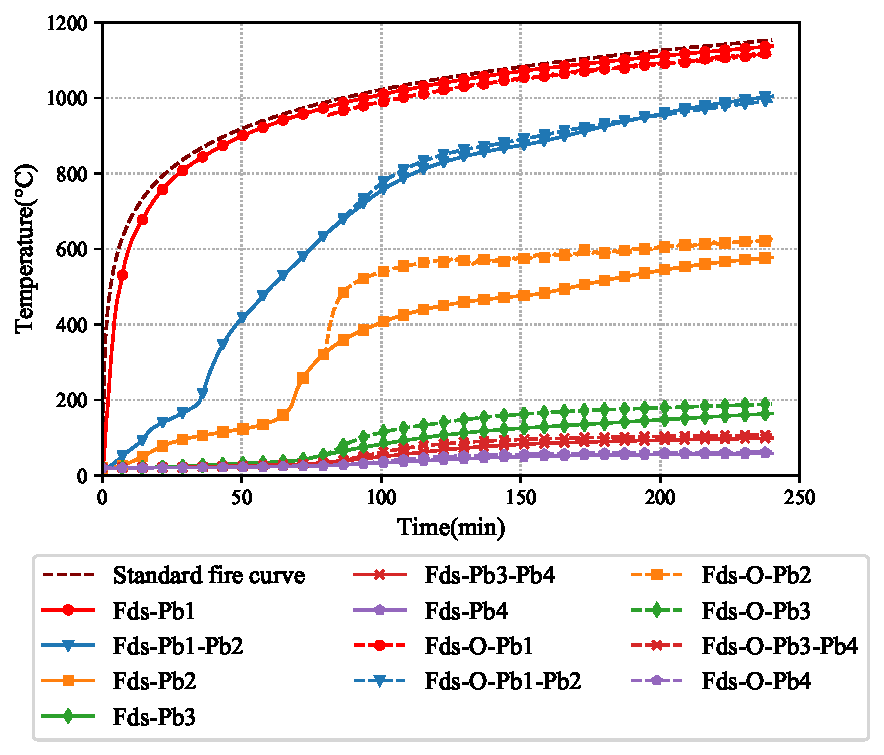
\includegraphics[width=\textwidth]{DS-70-075-2x16-AI-r1-PB.pdf}
		\caption{}
		\label{subfig:DS-70-075-2x16-AI-r1-PB}
	\end{subfigure}
	\begin{subfigure}[b]{0.6\textwidth}
		\centering
		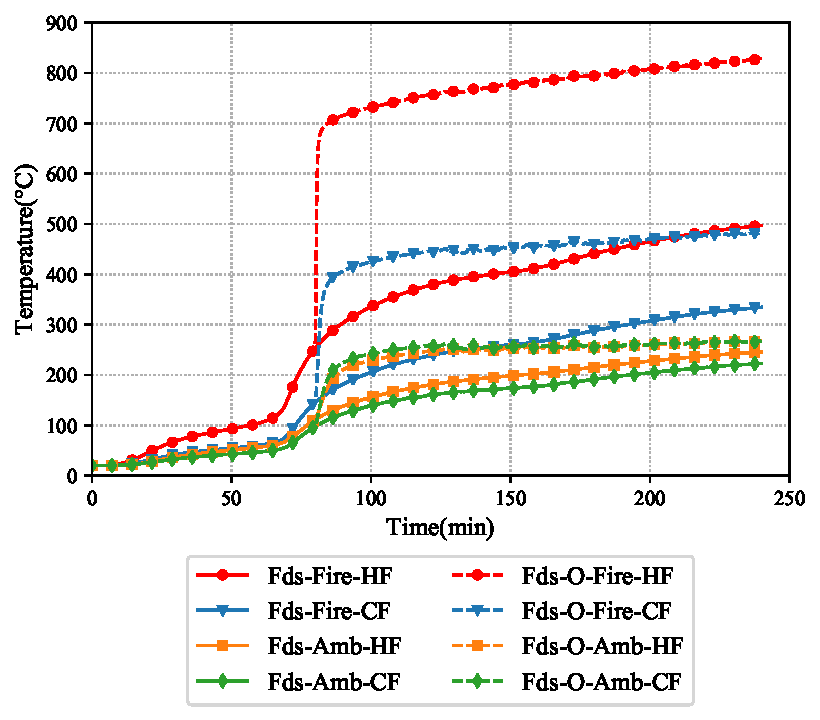
\includegraphics[width=\textwidth]{DS-70-075-2x16-AI-r1-Studs.pdf}
		\caption{}
		\label{subfig:DS-70-075-2x16-AI-r1-Studs}
	\end{subfigure}
	   \caption{Model DS-70-0.75-AI - Plasterboard and stud time-temperature curves of ambient cavity insulated double stud wall with 70 $\times$ 0.75 mm studs - (a) Plasterboard temperatures (b) Stud temperatures}
	   \label{fig:DS-70-075-2x16-AI-r1}
\end{figure} 

Insulating the ambient side cavity as in \Cref{subfig:DS-70-AI} exhibits a different time-temperature curve behaviour as shown in \Cref{fig:DS-70-075-2x16-AI-r1}. Based on fire Test-T7 in \Cref{ch:Fire} the model DS-70-0.75-AI had cavity insulation only on the ambient side. The fire side plasterboard interface (Fds-O-Pb1-Pb2) shown in \Cref{subfig:DS-70-075-2x16-AI-r1-PB} exhibited a similar behaviour to the that of the non-cavity insulated model. It is to note that the Fds-O-Pb1-Pb2 exhibited a similar trend in comparison with the Fds-Pb1-Pb2. This infers that the time-temperature curve behaviour on the fire side plasterboard interface of cavity insulated 70 mm double stud models are similar irrespective of the plasterboard open-up. However, the fire side cavity time-temperature curve (Fds-O-Pb2) exhibited a steep rise after 60 min of simulation unlike the non-cavity insulated model. This is attributed to the difference in ''SETPOINT" temperature for plasterboard opn-up initiation in the thermal model. Despite the plasterboard open-up all the ambient side time-temperature curves which includes Fds-O-Pb3, Fds-O-Pb3-Pb4 and Fds-O-PB4 recorded temperatures less than 200\degree C till the end of simulation. Models without plasterboard open-up also exhibited similar behaviour. This infers that the glass fibre cavity insulation on the ambient side has trapped the heat from the fire side resulting in lower ambient side plasterboard temperatures confirming the absence of insulation failure in the models. The lower time-temperature curve exhibited by the ambient side hot and cold flange temperatures for model DS-70-0.75-AI confirms the behaviour of heat entrapment on the fire side surfaces only as shown in \Cref{subfig:DS-70-075-2x16-AI-r1-Studs}. The effect of heat entrapment is further evident from the increased stud fire side hot flange temperatures (Fire-HF). This was evident in the model without plasterboard open-up wherein the Fds-Fire-HF recorded temperatures higher than the other flanges.
\begin{figure}[!htbp]
	\centering
	\begin{subfigure}[b]{0.6\textwidth}
		\centering
		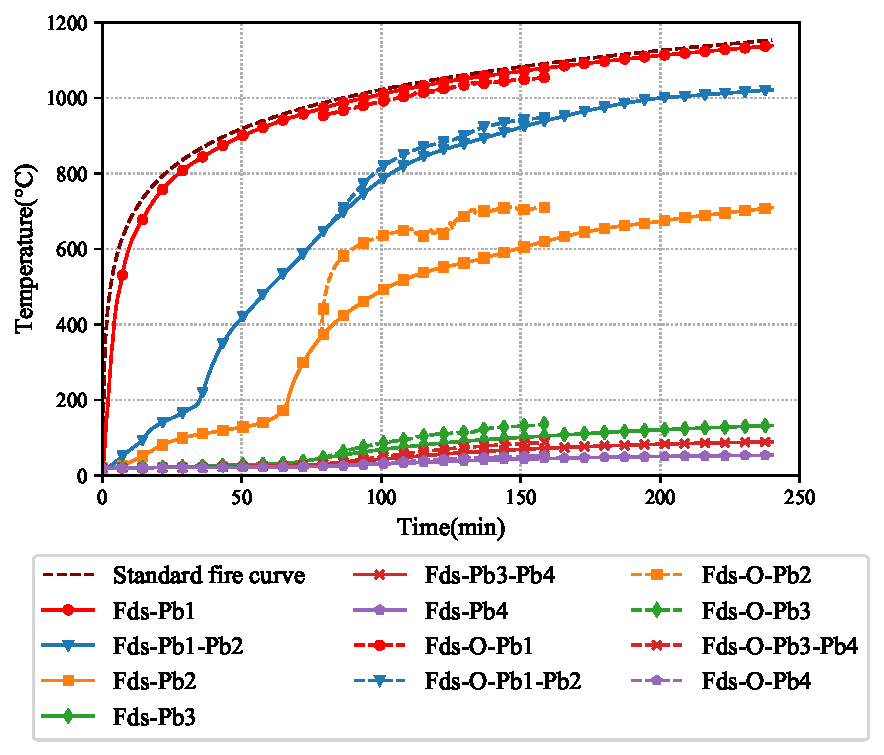
\includegraphics[width=\textwidth]{DS-70-075-2x16-BI-r2-PB.pdf}
		\caption{}
		\label{subfig:DS-70-075-2x16-BI-r2-PB}
	\end{subfigure}
	\begin{subfigure}[b]{0.6\textwidth}
		\centering
		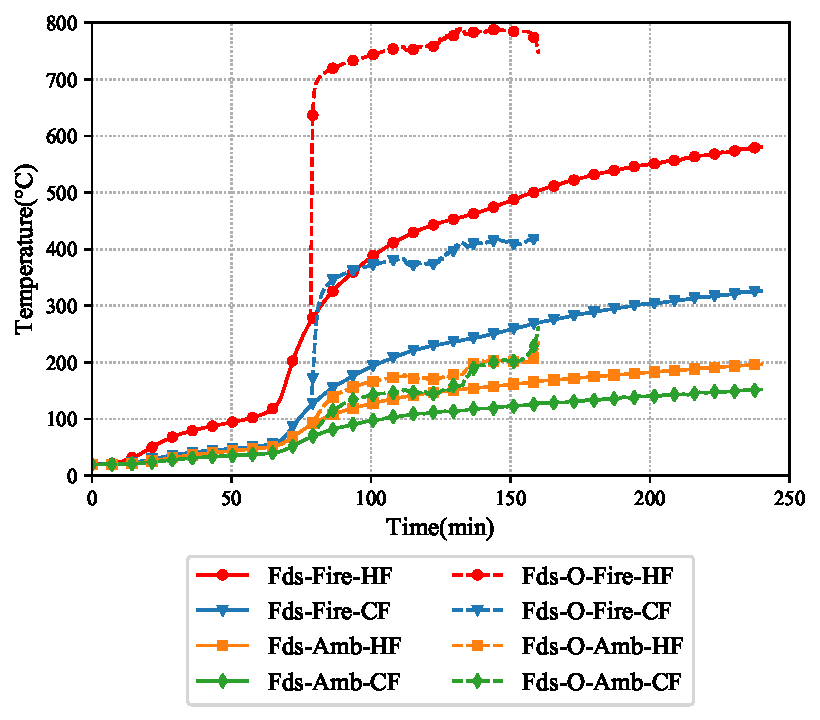
\includegraphics[width=\textwidth]{DS-70-075-2x16-BI-r2-Studs.pdf}
		\caption{}
		\label{subfig:DS-70-075-2x16-BI-r2-Studs}
	\end{subfigure}
	   \caption{Model DS-70-0.75-BI - Plasterboard and stud time-temperature curves of both cavity insulated double stud wall with 70 $\times$ 0.75 mm studs - (a) Plasterboard temperatures (b) Stud temperatures}
	   \label{fig:DS-70-075-2x16-BI-r2}
\end{figure} 

Providing cavity insulation on both the stud rows resulted in similar behaviour in the plasterboard and stud time-temperature curves similar to model DS-70-0.75-AI. Time-temperature curves of plasterboard and studs corresponding to model DS-70-0.75-2x16-BI are shown in \Cref{fig:DS-70-075-2x16-BI-r2}. The sudden increase in the plasterboard and stud time-temperature curves at plasterboard open-up is evident in the model with cavity insulation on both stud rows. Due to severe numerical instability the analysis was terminated at 160 min and could not be conducted for 240 min. However, the model without plasterboard open-up could be simulated for 240 min. Open-ups in the FDS thermal model causes severe numerical instability as explained in the FDS software manual (\cite{fds2013}) and requires multiple iterations in the case of non-convergence to arrive at the solution. As the model with plasterboard open-up resulted in temperatures above the limiting criteria, no further iterations were conducted on the model. 
\begin{figure}[!htbp]
	\centering
	\begin{subfigure}[b]{0.6\textwidth}
		\centering
		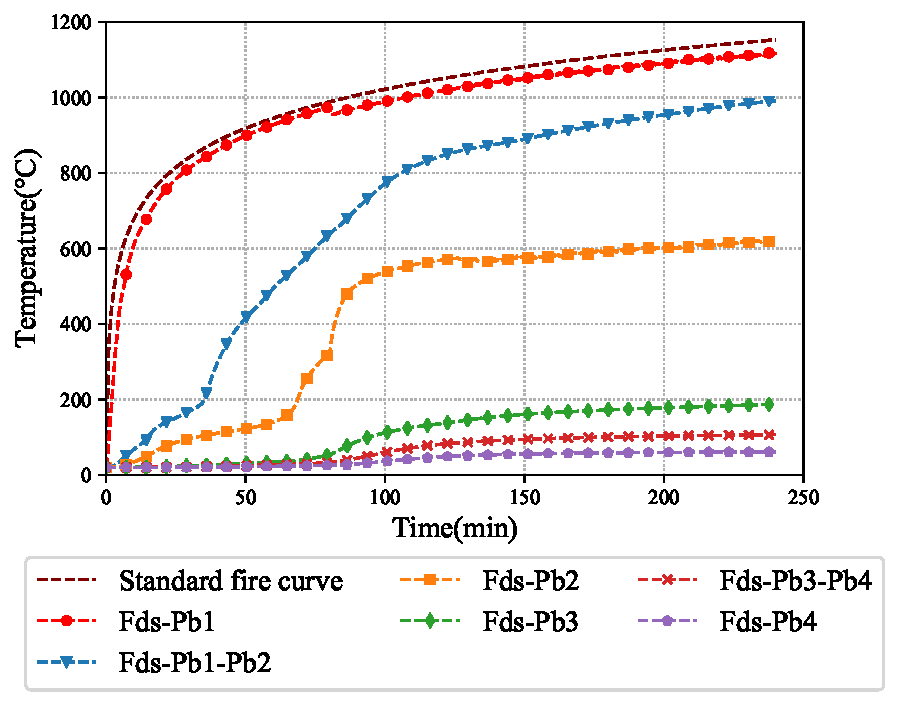
\includegraphics[width=\textwidth]{DS-70-095-2x16-AI-r1-PB.pdf}
		\caption{}
		\label{subfig:DS-70-095-2x16-AI-r1-PB}
	\end{subfigure}
	\begin{subfigure}[b]{0.6\textwidth}
		\centering
		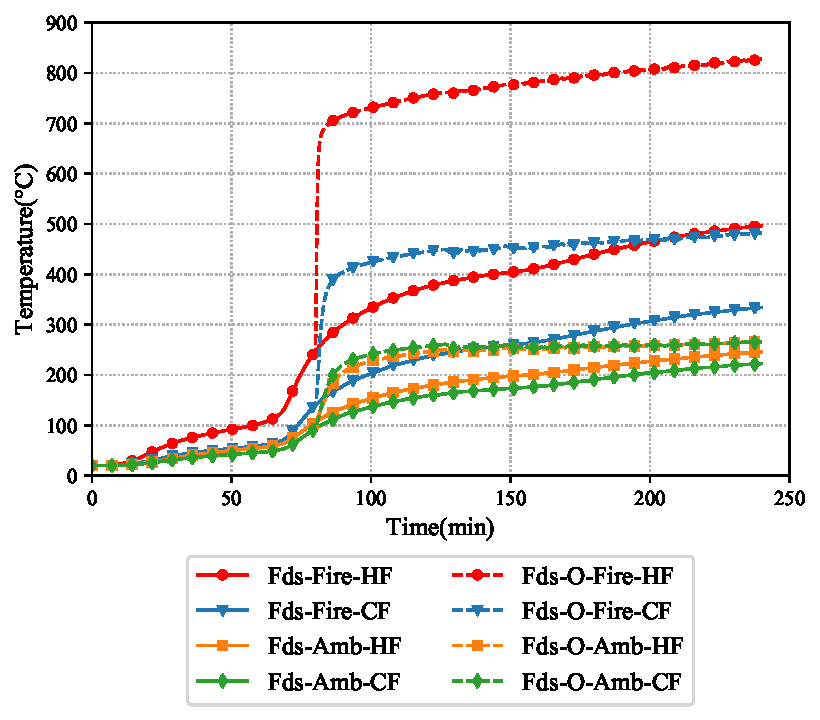
\includegraphics[width=\textwidth]{DS-70-095-2x16-AI-r1-Studs.pdf}
		\caption{}
		\label{subfig:DS-70-095-2x16-AI-r1-Studs}
	\end{subfigure}
	   \caption{Model DS-70-0.95-AI - Plasterboard and stud time-temperature curves of both cavity insulated double stud wall with 70 $\times$ 0.95 mm studs - (a) Plasterboard temperatures (b) Stud temperatures}
	   \label{fig:DS-70-095-2x16-AI-r1}
\end{figure} 
\begin{figure}[!htbp]
	\centering
	\begin{subfigure}[b]{0.6\textwidth}
		\centering
		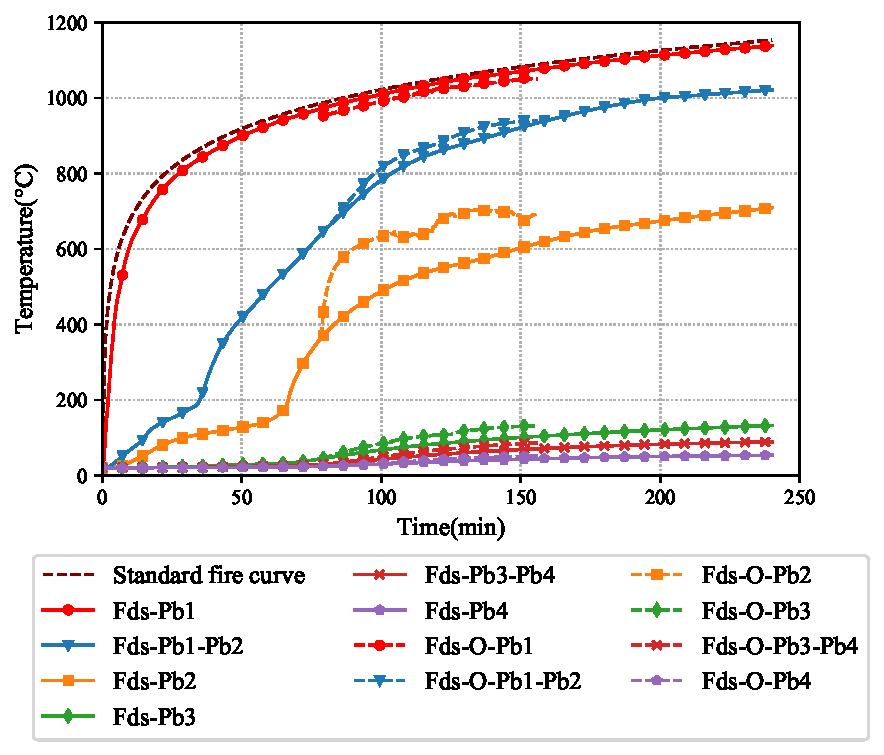
\includegraphics[width=\textwidth]{DS-70-095-2x16-BI-r1-PB.pdf}
		\caption{}
		\label{subfig:DS-70-095-2x16-BI-r1-PB}
	\end{subfigure}
	\begin{subfigure}[b]{0.6\textwidth}
		\centering
		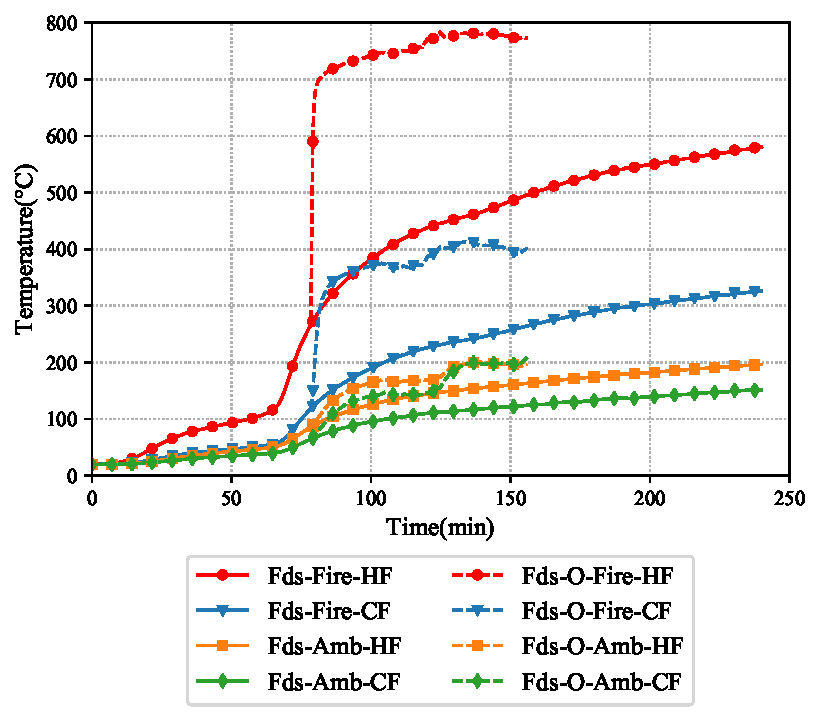
\includegraphics[width=\textwidth]{DS-70-095-2x16-BI-r1-Studs.pdf}
		\caption{}
		\label{subfig:DS-70-095-2x16-BI-r1-Studs}
	\end{subfigure}
	   \caption{Model DS-70-0.95-BI - Plasterboard and stud time-temperature curves of both cavity insulated double stud wall with 70 $\times$ 0.95 mm studs - (a) Plasterboard temperatures (b) Stud temperatures}
	   \label{fig:DS-70-095-2x16-BI-r1}
\end{figure} 

To determine the effect of cavity insulation on thicker studs, the model DS-70-0.95-2x16-BI was then created with 70 $\times$ 0.95 mm studs as shown in \Cref{subfig:DS-70-BI}. It is to note that fire Test-T4 was conducted with the same configuration as this model but without the cavity insulation. 
Similar to model DS-70-0.75-2x16-BI this model also suffered numerical instabilities leading to convergence issues and the thermal analysis could be simulated for 156 min only. However, the behaviour exhibited by the plasterboard and stud time-temperature curves as shown in \Cref{fig:DS-70-095-2x16-BI-r1} was similar to those exhibited by the DS-70-0.75-2x16-BI model. This infers that the effect of stud thickness does not result in significant changes in the time-temperature curves of cavity insulated double stud walls with 70 mm studs. This may be partly attributed by the effective cavity depth also. The effective cavity depth is 160 mm in this case which is less than the cavity depth of 200 mm generally available in double stud walls with 90 mm studs. Reduced cavity depth may result in faster heat transfer within the cavity from fire side to ambient side. Therefore the effect of stud thickness might not play a significant role in the temperature profile of the LSF wall. The model without the plasterboard open-up to simulate the non-load bearing conditions could be simulated for 240 min and is also shown in \Cref{fig:DS-70-095-2x16-BI-r1}. Similar to other models the time-temperature curves of the model without plasterboard open-up recorded temperatures less than the plasterboard open-up model.

\subsection{Double stud walls with 90 mm studs}

Like the double stud wall models with 70 mm studs attempts were made to predict the temperature profiles of double stud walls with 90 mm studs. An effective cavity depth of 200 mm was considered in the model (90$\times$2$+$20$=$200). Time-temperature curves of plasterboards and studs corresponding to double stud walls with 90 mm studs are discussed in this section. \Cref{fig:DS-90-075-2x16-AI-r1} shows the time-temperature curves of plasterboards and studs corresponding to double stud wall with 90 $\times$ 0.75 mm studs (DS-90-0.75-AI) with cavity insulation on the ambient stud rows. The non-cavity insulated models with the same configuration was considered for investigation through full-scale fire test in \Cref{ch:Fire} as Test-T2 and the thermal model predictions of the same was presented in \Cref{sec:thermal-model-non-cav} of \Cref{ch:FE-Thermal}.
\begin{figure}[!htbp]
	\centering
	\begin{subfigure}[b]{0.6\textwidth}
		\centering
		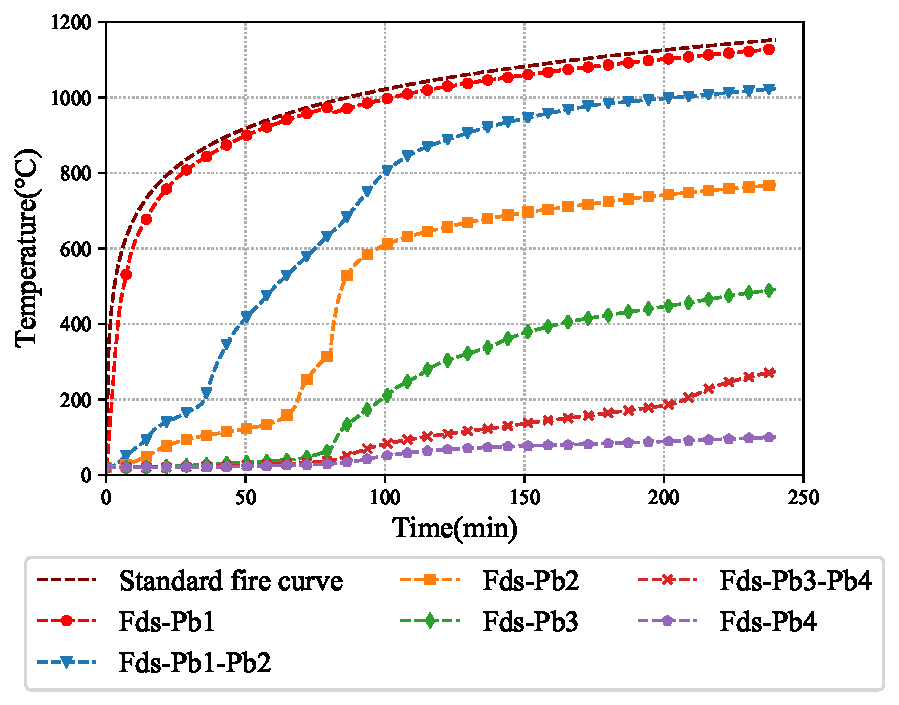
\includegraphics[width=\textwidth]{DS-90-075-2x16-AI-r1-PB.pdf}
		\caption{}
		\label{subfig:DS-90-075-2x16-AI-r1-PB}
	\end{subfigure}
	\begin{subfigure}[b]{0.6\textwidth}
		\centering
		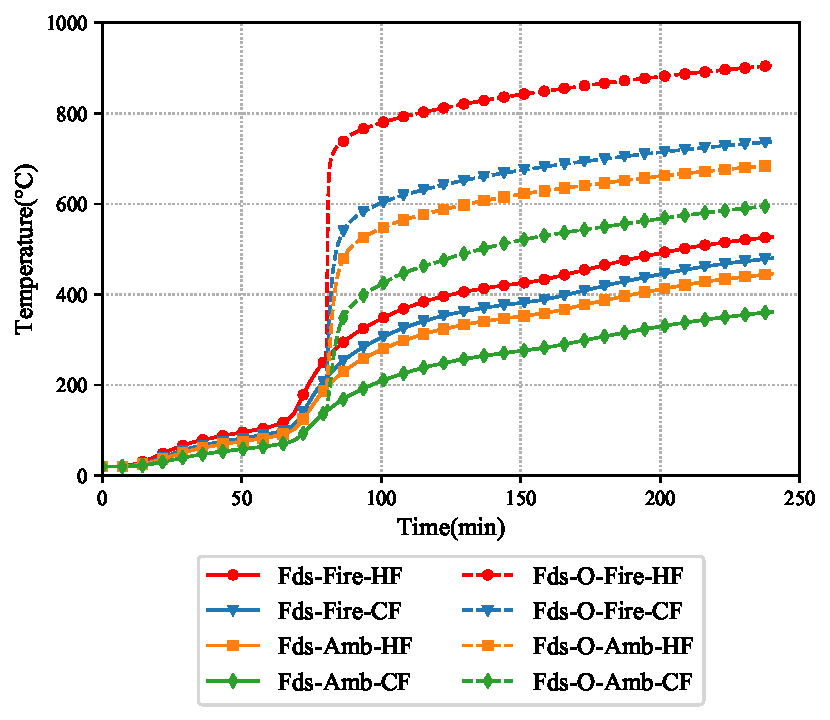
\includegraphics[width=\textwidth]{DS-90-075-2x16-AI-r1-Studs.pdf}
		\caption{}
		\label{subfig:DS-90-075-2x16-AI-r1-Studs}
	\end{subfigure}
	   \caption{Model DS-90-0.75-AI - Plasterboard and stud time-temperature curves of ambient cavity insulated double stud wall with 90 $\times$ 0.75 mm studs - (a) Plasterboard temperatures (b) Stud temperatures}
	   \label{fig:DS-90-075-2x16-AI-r1}
\end{figure}

The fire side interface plasterboard time-temperature curve (Fds-O-Pb1-Pb2) from model DS-90-0.75-AI shown in \Cref{subfig:DS-90-075-2x16-AI-r1-PB} exhibits a steep increase in the curve similar to the double stud wall models with 70 mm studs. This is witnessed in the model with plasterboard open-up (Fds-O-Pb1-Pb2). But the ambient side plasterboard temperatures (Fds-O-Pb3) are more in comparison with the double stud models with 70 mm studs. This is attributed by the glass fibre cavity insulation in the wall entrapping the heat flow within the cavity confirming the earlier claim. In the case of double stud wall with cavity insulation on the ambient side, there is no contact between the glass fibre insulation and the fire side plasterboards. This allows the heat to be transferred to the ambient side plasterboards and the insulation resulting in higher time-temperature curves in comparison with double stud wall with 70 mm studs. This is evident from the stud time-temperature curve shown in \Cref{subfig:DS-90-075-2x16-AI-r1-Studs}. The difference in the hot and cold flanges are minimal in the case of DS-90-0.75-AI. However, in the case of 70 mm double stud wall with ambient cavity insulation model DS-90-0.75-AI, the ambient side stud time-temperature curves shows very less difference and record similar temperatures as shown in \Cref{subfig:DS-70-095-2x16-AI-r1-Studs}. The maximum fire side hot flange temperature of Fds-Fire-HF was 527\degree C while it was 905\degree C for Fds-O-Fire-HF. 
\begin{figure}[!htbp]
	\centering
	\begin{subfigure}[b]{0.6\textwidth}
		\centering
		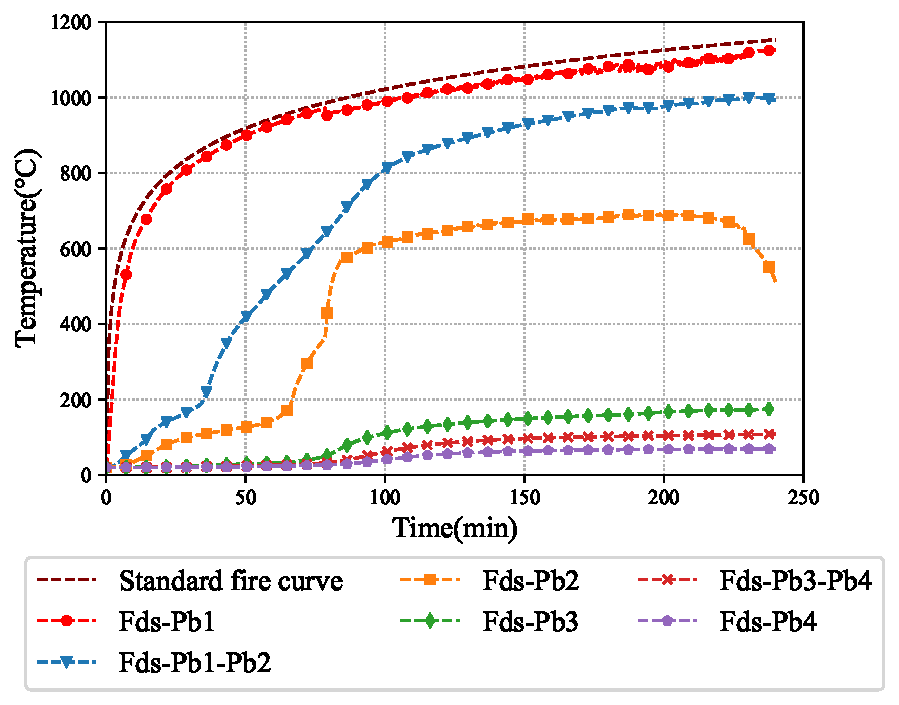
\includegraphics[width=\textwidth]{DS-90-075-2x16-BI-r2-PB.pdf}
		\caption{}
		\label{subfig:DS-90-075-2x16-BI-r2-PB}
	\end{subfigure}
	\begin{subfigure}[b]{0.6\textwidth}
		\centering
		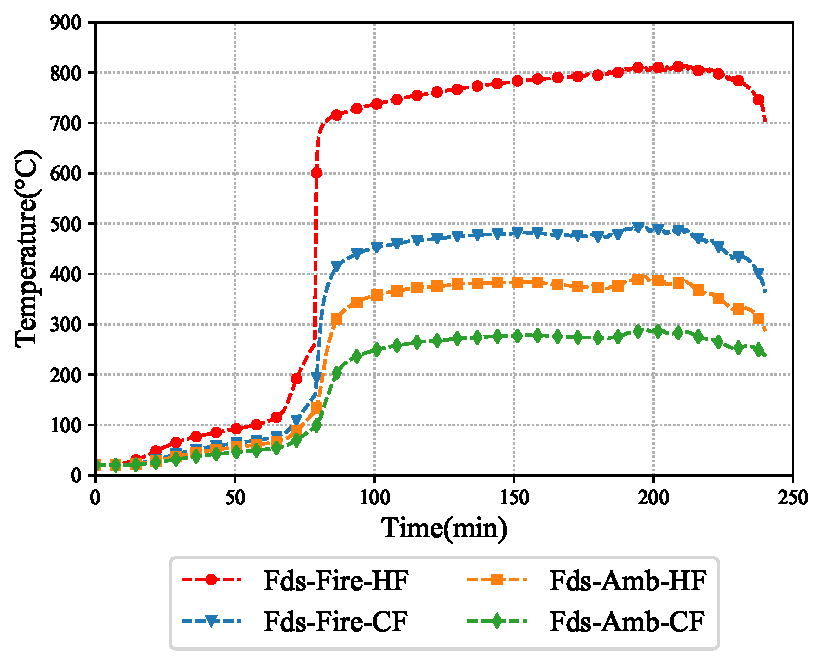
\includegraphics[width=\textwidth]{DS-90-075-2x16-BI-r2-Studs.pdf}
		\caption{}
		\label{subfig:DS-90-075-2x16-BI-r2-Studs}
	\end{subfigure}
	   \caption{Model DS-90-0.75-BI - Plasterboard and stud time-temperature curves of both cavity insulated double stud wall with 90 $\times$ 0.75 mm studs - (a) Plasterboard temperatures (b) Stud temperatures}
	   \label{fig:DS-90-075-2x16-BI-r2}
\end{figure}

In the case of 90 mm double stud wall with both cavity insulation model DS-90-0.75-BI, the time-temperature curve on the ambient side plasterboards were less than 200\degree C till the end of simulation as shown in \Cref{subfig:DS-90-075-2x16-BI-r2-PB}. This is in correlation with the time-temperature curves of both cavity insulated 70 mm double stud wall. Also, the difference between the fire side hot flange temperatures and the corresponding cold flange temperatures are significantly high in comparison with the ambient side cavity insulated walls and is shown in \Cref{subfig:DS-90-075-2x16-BI-r2-Studs}. The difference between fire side hot and cold flanges (Fds-O-Fire-HF and CF) was 136\degree C (551\degree$-$416\degree C) in the model without plasterboard open-up while the difference was 317\degree C (814\degree$-$497\degree C) in the model with plasterboard open-up. This shows the intensity of thermal load incident on the stud hot flange due to plasterboard open-up in cavity insulated 90 mm double stud LSF walls.   

\subsection{Shaftliner stud walls with 70 mm studs}

Due to the limitations in the testing set-up, shaftliner LSF walls could not be tested under load bearing conditions during experimental investigation. To overcome this limitation parametric study was conducted on the shaftliner LSF walls systems for 70 and 90 mm deep studs wherein shaftliner walls with 70 mm studs are discussed in this section. Firstly, the results from the FDS thermal analysis are discussed. Later, the stud temperatures were used to determine the failure time of the test wall under load bearing conditions through the sequentially coupled temperature displacement analysis which was validated in \Cref{ch:FE-Structural}. This sections details the thermal analysis results on shaftliner LSF walls with 70 mm studs as shown in \Cref{fig:SL-70-90-parametric} (a) and (b). An effective cavity depth of 156 mm was considered in the model (70$\times$2$+$16$=$156). 
\begin{figure}[!htbp]
	\centering
	\begin{subfigure}[b]{0.6\textwidth}
		\centering
		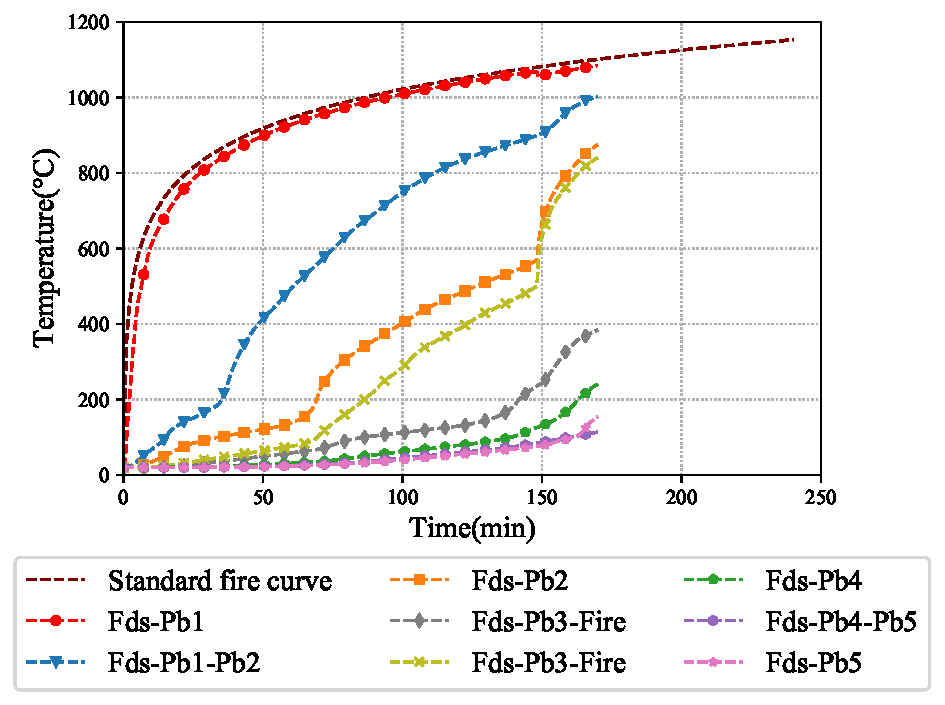
\includegraphics[width=\textwidth]{SL-70-075-2x16-r1-PB.pdf}
		\caption{}
		\label{subfig:SL-70-075-2x16-r1-PB}
	\end{subfigure}
	\begin{subfigure}[b]{0.6\textwidth}
		\centering
		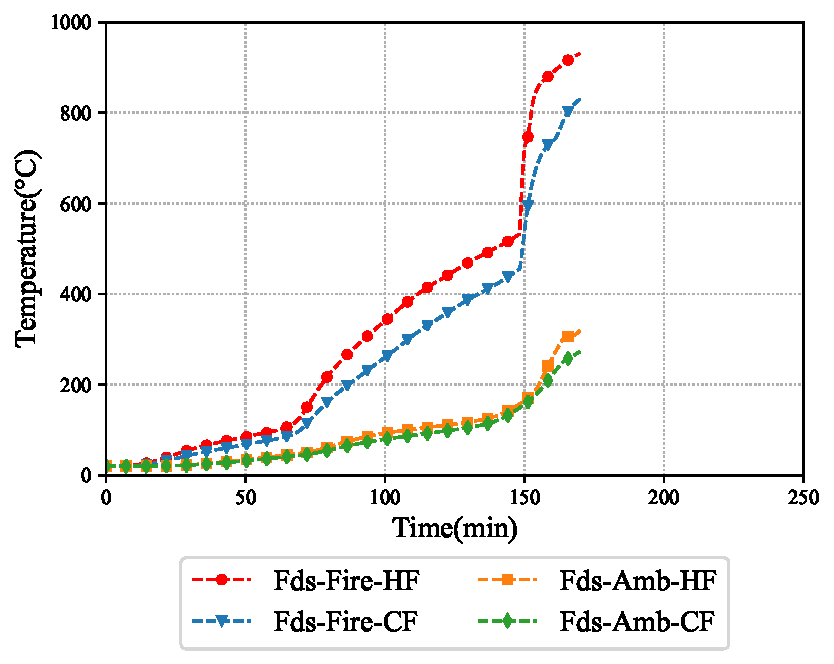
\includegraphics[width=\textwidth]{SL-70-075-2x16-r1-Studs.pdf}
		\caption{}
		\label{subfig:SL-70-075-2x16-r1-Studs}
	\end{subfigure}
	   \caption{Model SL-70-0.75 - Plasterboard and stud time-temperature curves of non-cavity insulated shaftliner wall with 70 $\times$ 0.75 mm studs - (a) Plasterboard temperatures (b) Stud temperatures}
	   \label{fig:SL-70-075-2x16-r1}
\end{figure}

\Cref{subfig:SL-70-075-2x16-r1-PB} shows the plasterboard time-temperature curve corresponding to the non-cavity insulated shaftliner model SL-70-0.75 similar to the configuration shown in \Cref{subfig:SL-70}. Severe non-linearity was experienced during thermal analysis leading to convergence issues and the model was simulated for 170 min. This is because of the consideration of plasterboard open-up in the model similar to the double stud walls. However, the plasterboard open-up has resulted in a steep inclination after 150 min. This is evident in the fire and ambient side plasterboard time temperature curves (Fds-O-Pb1 and Fds-O-Pb3-Fire and Amb) shown in \Cref{subfig:SL-70-075-2x16-r1-PB}. The plasterboard interface time-temperature curve Fds-O-Pb1-Pb2 tend to reach the input fire curve after 150 min of simulation because of the small effective cavity depth of 70 mm. This is also visible in the corresponding fire side cavity Fds-O-Pb2 time-temperature curve and in the plasterboard between the cavity Fds-O-Pb3-Fire and Fds-O-Pb3-Amb. The steep increase in the time-temperature curve is also visible on the ambient side plasterboards (Fds-O-Pb4 and Pb5) but is subtle in comparison with the fire side. The model without plasterboard open-up did not experience convergence issue and was able to be simulated for 240 min. The corresponding time-temperature curve to simulate the thermal behaviour in non-load bearing shaftliner LSF walls is also compared along with the plasterboard open-up models. The stud time-temperature curves exhibit a steep rise in the fire side hot flange temperatures as shown in \Cref{subfig:SL-70-075-2x16-r1-Studs}. The fire side hot and cold flange temperatures (Fds-Fire-HF and CF) exceeded 800\degree C after 160 min which is higher than the limiting temperature for stud failure under all load ratios proposed by \citet{Gunalan2013a}. Considering the critical hot flange temperature no further iterations were conducted for the model SL-70-0.75. However, the model without plasterboard open-up could be simulated for 240 min.
\begin{figure}[!htbp]
	\centering
	\begin{subfigure}[b]{0.6\textwidth}
		\centering
		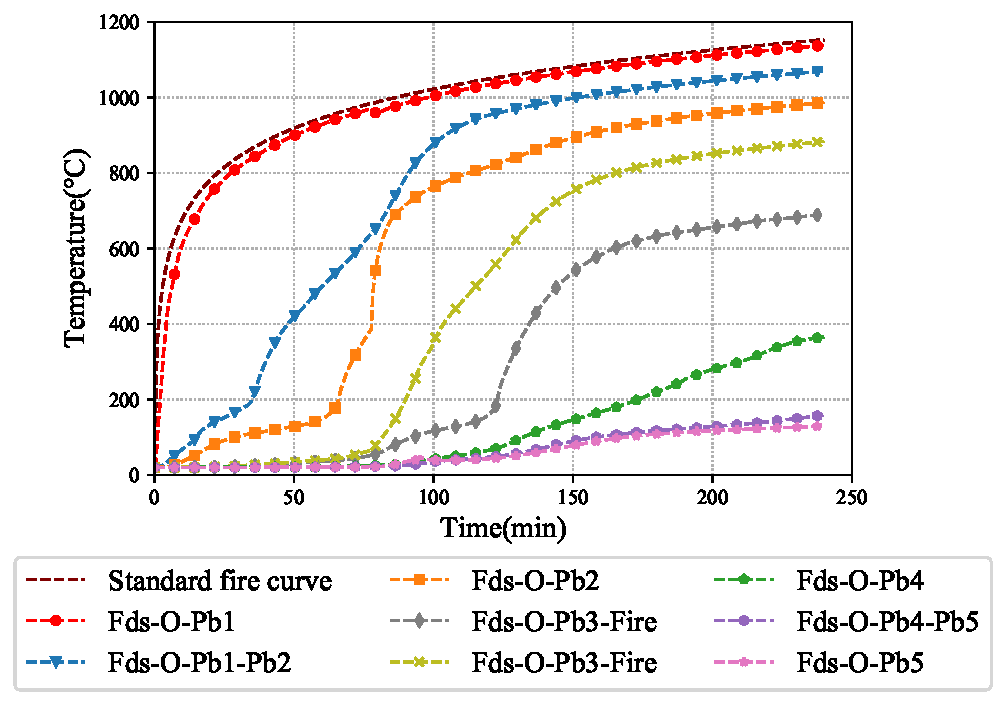
\includegraphics[width=\textwidth]{SL-70-075-2x16-FI-r1-PB.pdf}
		\caption{}
		\label{subfig:SL-70-075-2x16-FI-r1-PB}
	\end{subfigure}
	\begin{subfigure}[b]{0.6\textwidth}
		\centering
		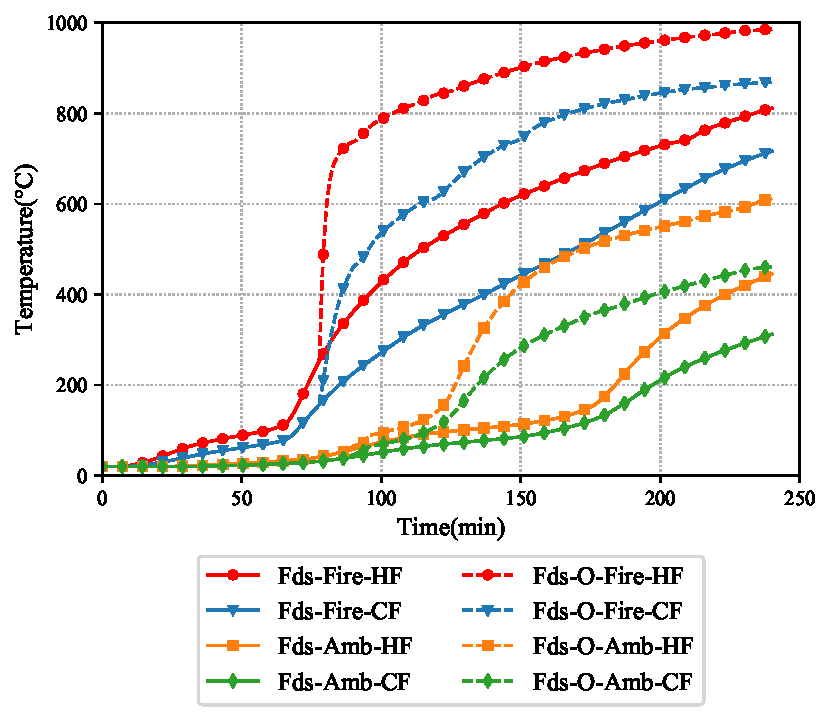
\includegraphics[width=\textwidth]{SL-70-075-2x16-FI-r1-Studs.pdf}
		\caption{}
		\label{subfig:SL-70-075-2x16-FI-r1-Studs}
	\end{subfigure}
	   \caption{Model SL-70-0.75-FI - Plasterboard and stud time-temperature curves of cavity insulated shaftliner wall with 70 $\times$ 0.75 mm studs - (a) Plasterboard temperatures (b) Stud temperatures}
	   \label{fig:SL-70-075-2x16-FI-r1}
\end{figure}

\Cref{fig:SL-70-075-2x16-FI-r1} shows the time-temperature curves from model SL-70-0.75-FI. The model was simulated with full cavity insulation as shown in \Cref{subfig:SL-70-BI}. Models with cavity insulation only on the fire side cavity was not considered for the FDS thermal parametric analysis. This is because in general construction practice shaftliner walls are used with full cavity insulation to achieve the desired acoustic ratings. Also, providing cavity insulation only on the fire side cavity will make the shaftliner wall behave like a single stud wall. This is because of the heat entrapment in cavity insulated LSF walls. \Cref{subfig:SL-70-075-2x16-FI-r1-PB} shows the time-temperature curve of plasterboards corresponding to model SL-70-0.75-FI. The Fds-Pb1-Pb2 curve exhibits a steep rise tending to match the input ISO 834 time-temperature curve. This infers the entrapment of heat by the cavity insulation within the fire side plasterboards. This behaviour is exhibited by the Fds-O-Pb1-Pb2 curve which confirms the earlier claim in double stud wall models that the time-temperature curve on the fire side plasterboard interface is similar irrespective of the plasterboard open-up. 
\begin{figure}[!htbp]
	\centering
	\begin{subfigure}[b]{0.6\textwidth}
		\centering
		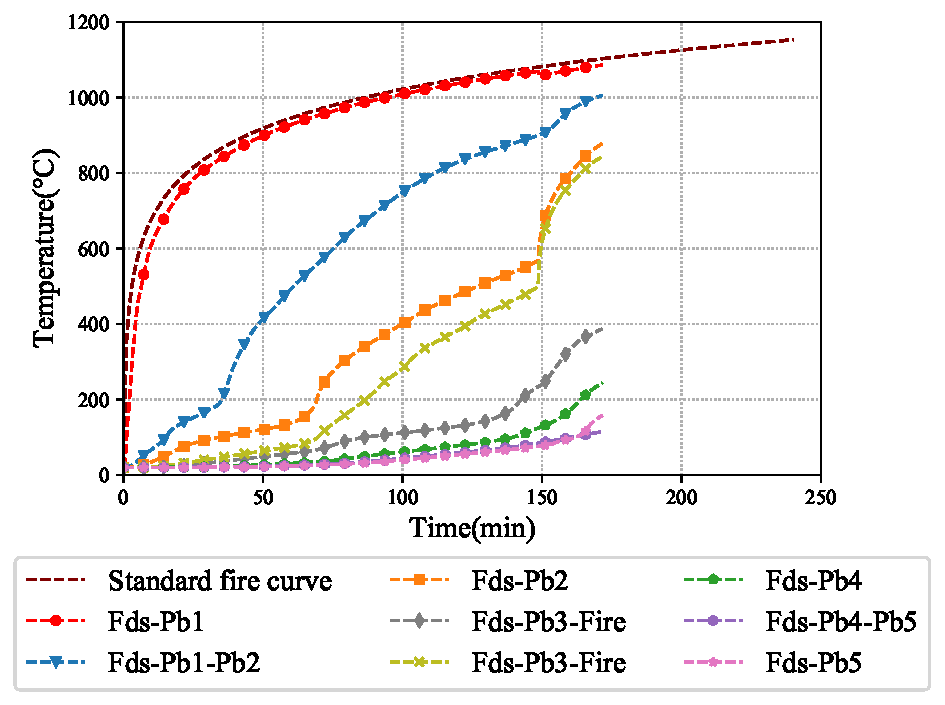
\includegraphics[width=\textwidth]{SL-70-095-2x16-r1-PB.pdf}
		\caption{}
		\label{subfig:SL-70-095-2x16-r1-PB}
	\end{subfigure}
	\begin{subfigure}[b]{0.6\textwidth}
		\centering
		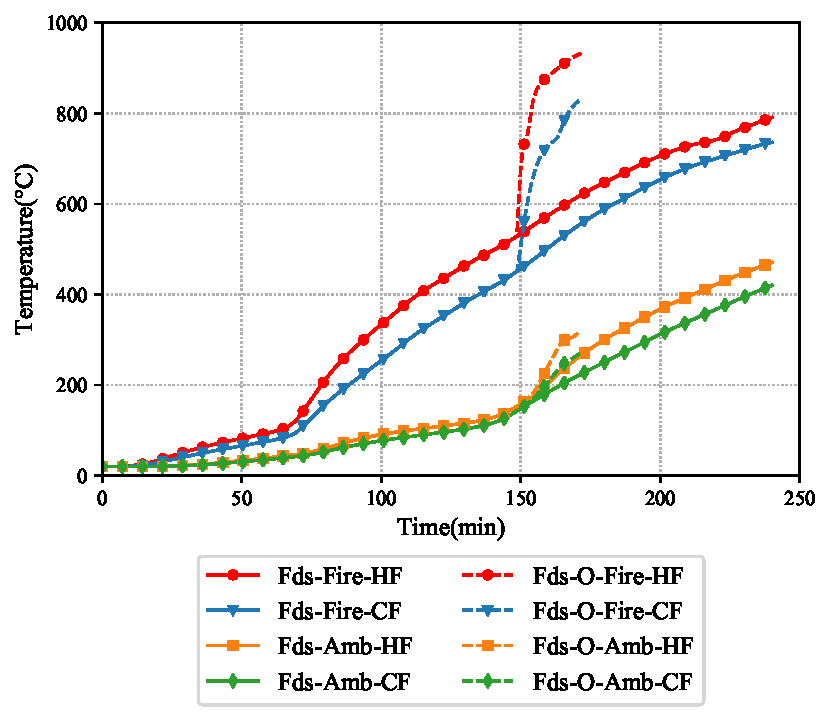
\includegraphics[width=\textwidth]{SL-70-095-2x16-r1-Studs.pdf}
		\caption{}
		\label{subfig:SL-70-095-2x16-r1-Studs}
	\end{subfigure}
	   \caption{Model SL-70-0.95 - Plasterboard and stud time-temperature curves of non-cavity insulated shaftliner wall with 70 $\times$ 0.95 mm studs - (a) Plasterboard temperatures (b) Stud temperatures}
	   \label{fig:SL-70-095-2x16-r1}
\end{figure}

Similar trend was observed on the middle plasterboard layer within the cavity. However, the non-plasterboard open-up model exhibited a gradual increase till the end of simulation. The ambient side plasterboard interface Fds-O-Pb4-Pb5 and ambient side plasterboard Fds-O-Pb5 time-temperature curves were less than 200\degree C till the end of simulation. The stud time-temperature curve shown in \Cref{subfig:SL-70-075-2x16-FI-r1-Studs} also exhibited the steep gradient on the fire side hot and cold flanges (Fire-HF and CF). The difference between the fire side hot and cold flanges (Fds-O-Fire-HF and CF) in comparison with the ambient side hot and cold flanges (Fds-O-Amb-HF and CF) was large as a result of cavity insulation. This behaviour was also observed in the double stud wall models. The stud time-temperature curves were also similar in the models without plasterboard open-up till the open-up time. The large difference in the fire and ambient side studs was also evident in the Fds-Fire-HF and CF and Fds-Amb-HF and CF time-temperature curves. It is to note that, in the case of double stud wall model, steep inclination in the time-temperature curve was predominant in the fire side hot flange(Fds-O-Fire-HF) only. The inclination in Fds-O-Fire-CF, Fds-O-Amb-HF and CF time-temperature curves were not large in comparison with the Fds-O-Fire-HF in the case of double stud LSF walls. But, in the case of shaftliner walls, both the Fds-O-Fire-HF and CF exhibit a steep inclination in the time-temperature curve. This is influenced by the middle plasterboard layer containing the heat within the fire side cavity. This effect of steep inclination in the fire side stud time-temperature curves is further influenced by the presence of cavity insulation and was also present in the models without plasterboard open-up. 
\begin{figure}[!htbp]
	\centering
	\begin{subfigure}[b]{0.6\textwidth}
		\centering
		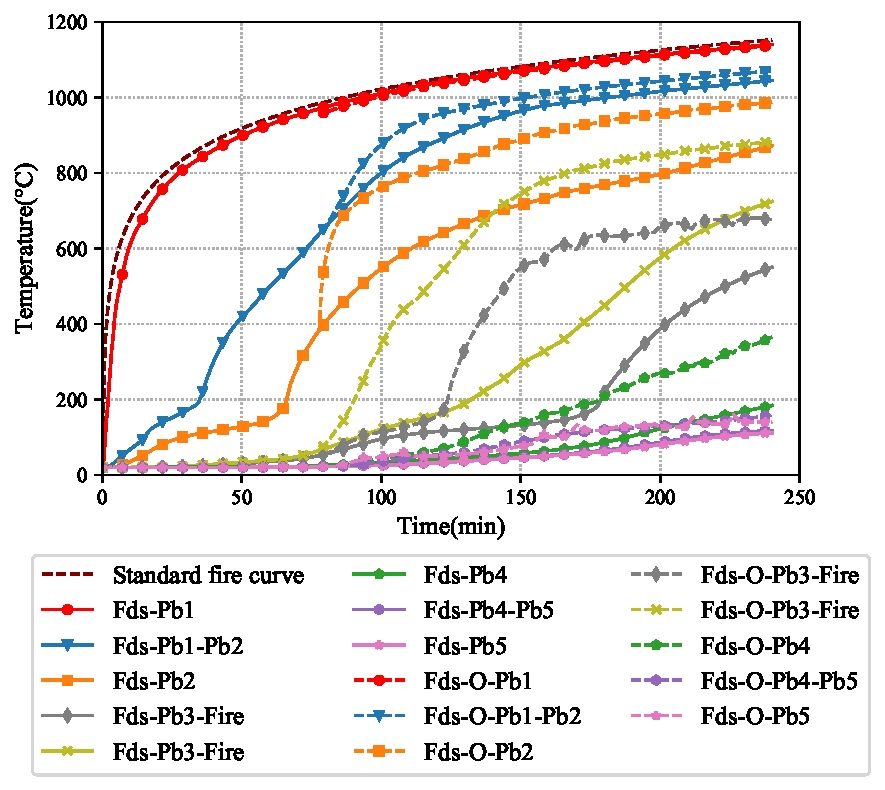
\includegraphics[width=\textwidth]{SL-70-095-2x16-FI-r1-PB.pdf}
		\caption{}
		\label{subfig:SL-70-095-2x16-FI-r1-PB}
	\end{subfigure}
\begin{subfigure}[b]{0.6\textwidth}
	\centering
	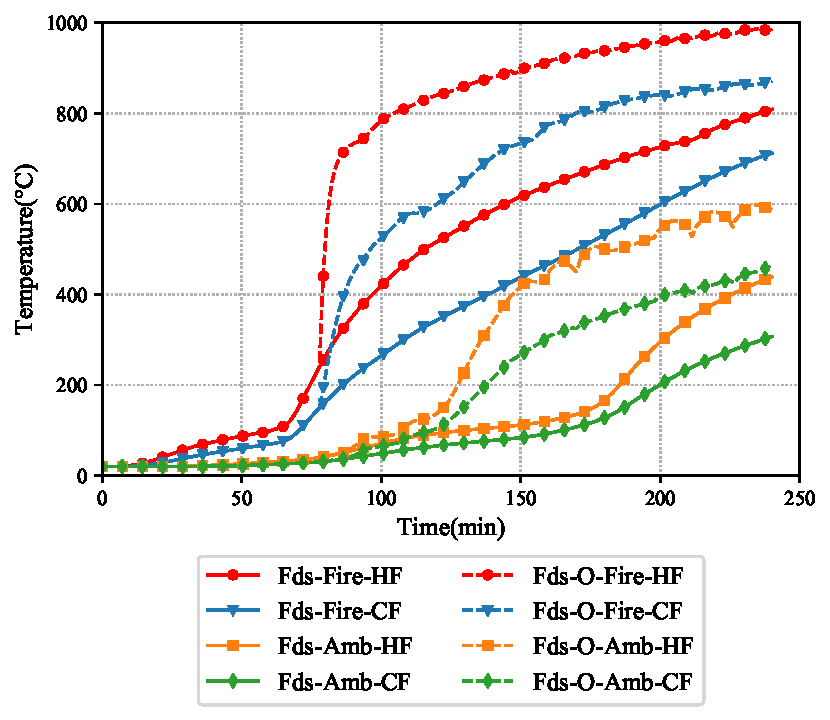
\includegraphics[width=\textwidth]{SL-70-095-2x16-FI-r1-Studs.pdf}
	\caption{}
	\label{subfig:SL-70-095-2x16-FI-r1-Studs}
\end{subfigure}
   \caption{Model SL-70-0.95-FI - Plasterboard and stud time-temperature curves of cavity insulated shaftliner wall with 70 $\times$ 0.95 mm studs - (a) Plasterboard temperatures (b) Stud temperatures}
   \label{fig:SL-70-095-2x16-FI-r1}
\end{figure}

The thickness of the 70 mm deep stud shaftliner model was changed from 0.75 mm to 0.95 mm and thermal analysis was conducted. Time-temperature curves of plasterboard and stud corresponding to the model SL-70-0.95 and SL-70-0.95-FI are shown in \Cref{fig:SL-70-095-2x16-r1,fig:SL-70-095-2x16-FI-r1}. The non-cavity insulated model also experienced numerical instability and the thermal model was simulated for 172 min. It is evident from the time-temperature curves that there is no significant difference in comparison with the time-temperature curves from the cavity insulated model SL-70-0.75-FI. This infers that the effect of stud thickness did not significantly influence the heat transfer within the wall cavity in shaftliner LSF walls. This inference also holds good in the case of models without plasterboard open-up. No further iterations were conducted on the plasterboard open-up model as the critical fire side stud hot flange temperature (Fds-O-Fire-HF) has already exceeded 800\degree C which is more than the limiting temperature under any load bearing condition under the general LR of 0.2 to 0.7. 

\subsection{Shaftliner stud walls with 90 mm studs}

Shaftliner wall models were created with 90 mm deep 0.75 and 0.95 mm thick studs as shown in \Cref{subfig:SL-90-BI} and are discussed in this section. The effective cavity depth considered in the model was 196 (90$\times$2$+$16$=$196). \Cref{fig:SL-90-075-2x16-FI-r2} shows the time-temperature curves of studs and plasterboard from cavity insulated shaftliner model with 90 $\times$ 0.75 mm studs. Non-cavity insulated shaftliner wall 90 $\times$ 0.75 mm studs was investigated in the experimental study as Test-T8 in \Cref{ch:Fire} and thermal model predictions for the same was conducted in \Cref{ch:FE-Thermal}. The steep increase in the plasterboard interface time-temperature curve (Fds-O-Pb1-Pb2) was observed in the model with plasterboard open-up tending to reach the input ISO 834 time-temperature curve as shown in \Cref{subfig:SL-90-075-2x16-FI-r2-PB}. Non-cavity insulated shaftliner model (SL-90-0.75) with plasterboard open-up experienced severe instability similar to the previous plasterboard open-up models. However, the model without plasterboard open-up could be simulated for 240 min. The Fds-O-Pb3-Fire plasterboard time-temperature curve corresponding to the middle fire side plasterboard surface exhibited a steep increase on the curve which was similar to the shaftliner models with 70 mm deep studs. This infers that irrespective of the stud depth used in the shaftliner LSF wall configuration, plasterboard open-up will result in direct exposure of heat into the cavity despite the provision of cavity insulation. This results in sudden increase in the fire side hot flange (Fds-O-Fire-HF and CF) time-temperature curves as shown in \Cref{subfig:SL-90-075-2x16-FI-r2-Studs}. However, in the case of the model without plasterboard open-up the hot flange temperature increases steadily. It is to note that the slope of the Fds-Fire-HF is higher in the case of shaftliner walls in comparison with the double stud walls as shown in \Cref{fig:fds-output-pb-studs-t2} in \Cref{ch:FE-Thermal}. This increased slope in the time-temperature curve is contributed by the middle plasterboard layer absorbing the heat within the cavity thereby increasing the fire side stud hot and cold flange temperatures. This phenomenon was also reported in the experimental investigation in \Cref{ch:Fire} and was also simulated by the developed FDS thermal model in \Cref{ch:FE-Thermal}. Parametric model results also affiliates this claim confirming the credibility of the developed FDS thermal model.  
\begin{figure}[!htbp]
	\centering
	\begin{subfigure}[b]{0.6\textwidth}
		\centering
		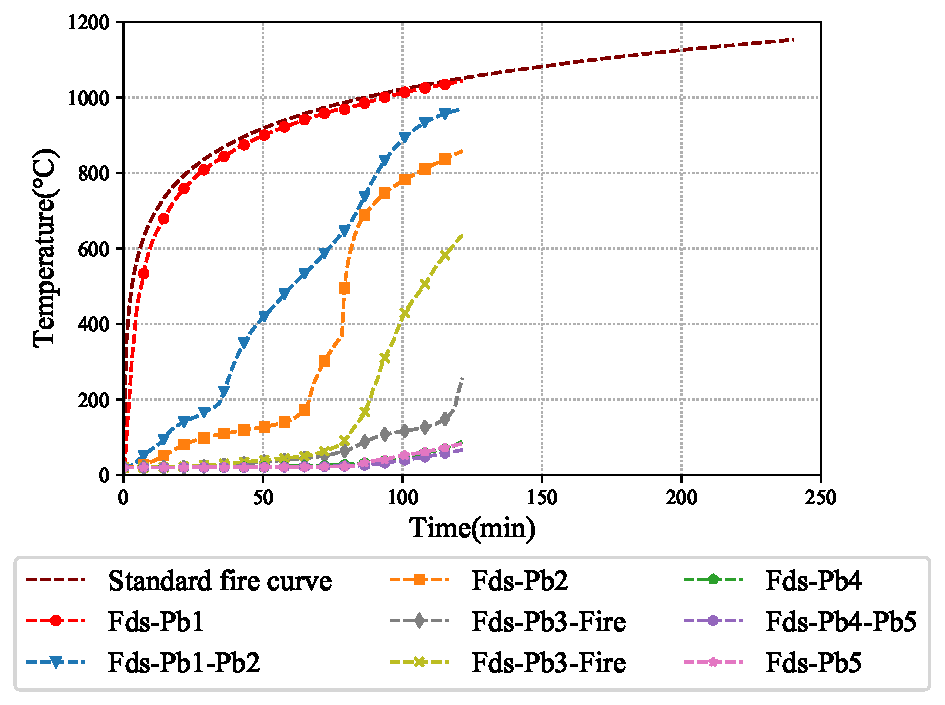
\includegraphics[width=\textwidth]{SL-90-075-2x16-FI-r2-PB.pdf}
		\caption{}
		\label{subfig:SL-90-075-2x16-FI-r2-PB}
	\end{subfigure}
	\begin{subfigure}[b]{0.6\textwidth}
		\centering
		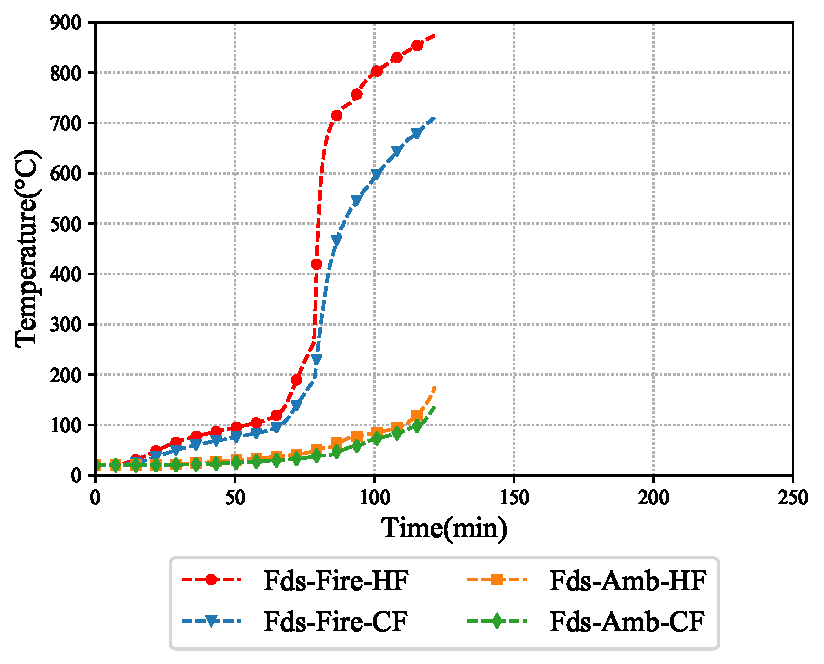
\includegraphics[width=\textwidth]{SL-90-075-2x16-FI-r2-Studs.pdf}
		\caption{}
		\label{subfig:SL-90-075-2x16-FI-r2-Studs}
	\end{subfigure}
	   \caption{Model SL-90-0.75-FI - Plasterboard and stud time-temperature curves of cavity insulated shaftliner wall with 90 $\times$ 0.75 mm studs - (a) Plasterboard temperatures (b) Stud temperatures}
	   \label{fig:SL-90-075-2x16-FI-r2}
\end{figure}

\Cref{fig:SL-90-095-2x16-r1,fig:SL-90-095-2x16-FI-r2} shows the time-temperature curves from thermal models on non-cavity insulated and cavity insulated shaftliner walls with 90 $\times$ 0.95 mm studs. Numerical instability was observed on both the models leading to a simulation time of 174 min for con-cavity insulated shaftliner model SL-90-0.95 and 122 min for cavity insulated shaftliner model SL-90-0.95-FI. Plasterboard time-temperature curves of non-cavity insulated model are similar till the plasterboard open-up after which a steep increase in the time-temperature curves are observed as shown in \Cref{subfig:SL-90-095-2x16-r1-PB}. Despite the plasterboard open-up the ambient side plasterboard interface (Fds-O-Pb3-Pb4) and the ambient side plasterboard (Fds-O-Pb4) recorded temperatures less than 200\degree C which confirms the absence of insulation failure in the model SL-90-0.95. This observation was also similar in the cavity insulated shaftliner model SL-90-0.95-FI. As the ''SETPOINT" temperatures are lower in the case of cavity insulated wall models the steep increase in the time-temperature curve is noticed earlier during simulation in comparison with the non-cavity insulated model. 
\begin{figure}[!htbp]
	\centering
	\begin{subfigure}[b]{0.6\textwidth}
		\centering
		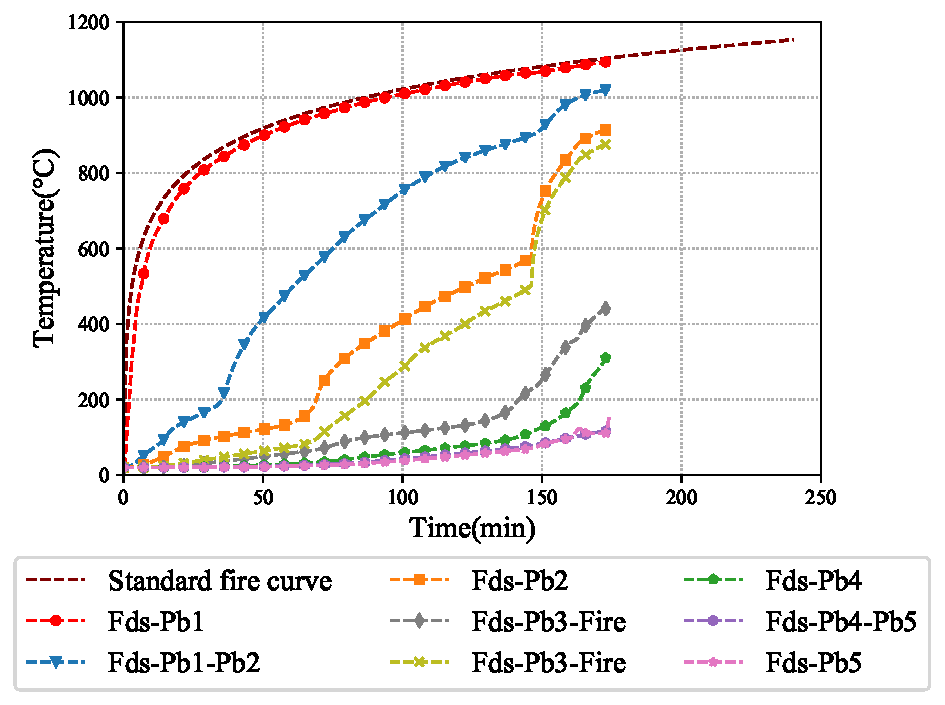
\includegraphics[width=\textwidth]{SL-90-095-2x16-r1-PB.pdf}
		\caption{}
		\label{subfig:SL-90-095-2x16-r1-PB}
	\end{subfigure}
	\begin{subfigure}[b]{0.6\textwidth}
		\centering
		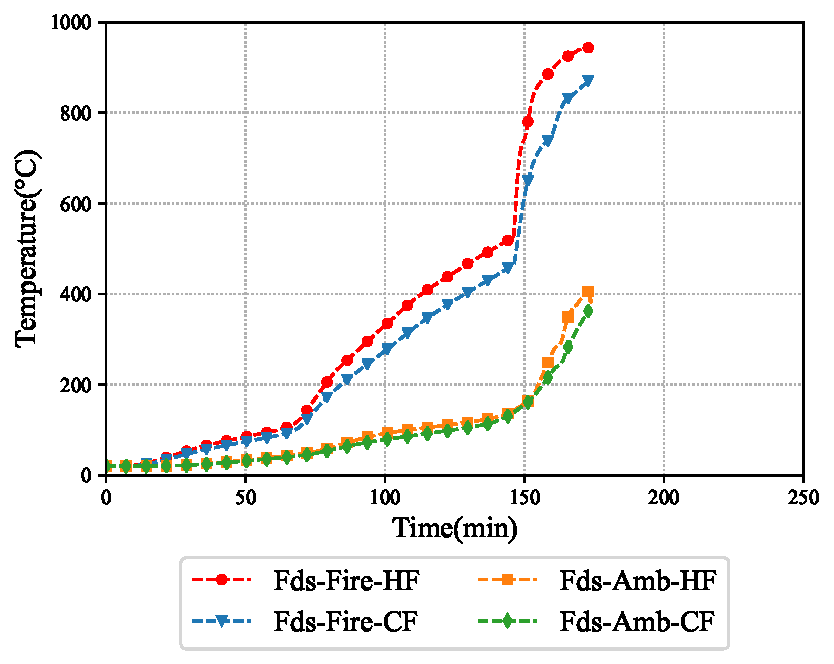
\includegraphics[width=\textwidth]{SL-90-095-2x16-r1-Studs.pdf}
		\caption{}
		\label{subfig:SL-90-095-2x16-r1-Studs}
	\end{subfigure}
	   \caption{Model SL-90-0.95 - Plasterboard and stud time-temperature curves of non-cavity insulated shaftliner wall with 90 $\times$ 0.95 mm studs - (a) Plasterboard temperatures (b) Stud temperatures}
	   \label{fig:SL-90-095-2x16-r1}
\end{figure}
\begin{figure}[!htbp]
	\centering
	\begin{subfigure}[b]{0.6\textwidth}
		\centering
		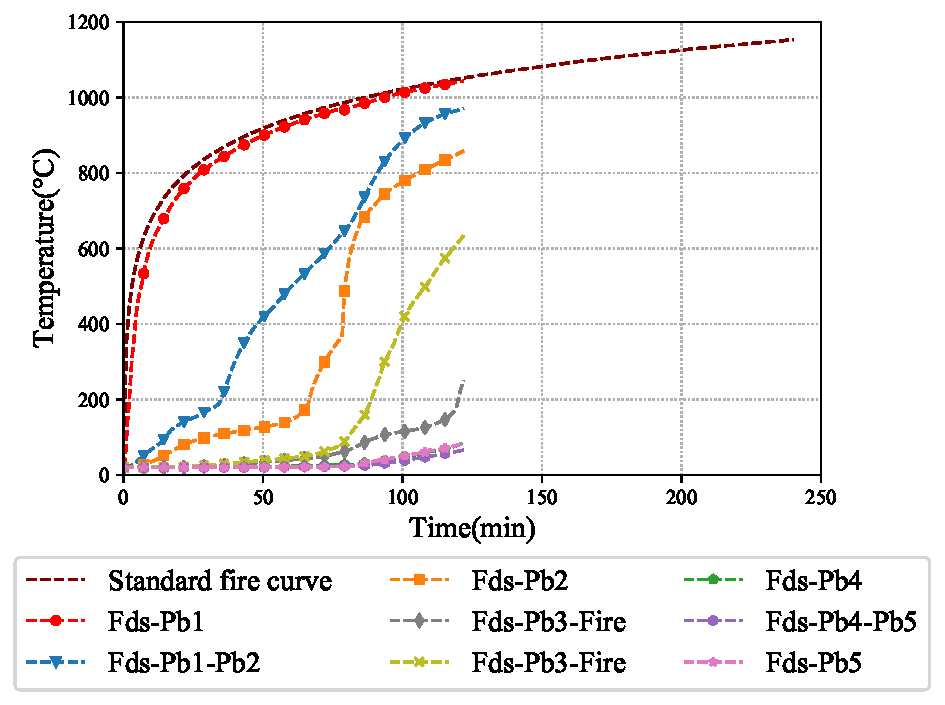
\includegraphics[width=\textwidth]{SL-90-095-2x16-FI-r2-PB.pdf}
		\caption{}
		\label{subfig:SL-90-095-2x16-FI-r2-PB}
	\end{subfigure}
	\begin{subfigure}[b]{0.6\textwidth}
		\centering
		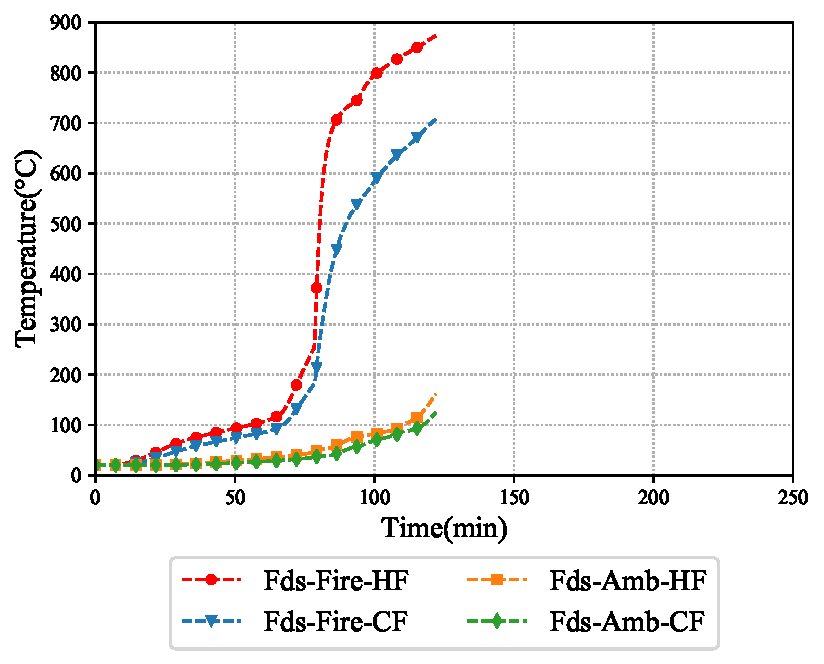
\includegraphics[width=\textwidth]{SL-90-095-2x16-FI-r2-Studs.pdf}
		\caption{}
		\label{subfig:SL-90-095-2x16-FI-r2-Studs}
	\end{subfigure}
	   \caption{Model SL-90-0.95-FI - Plasterboard and stud time-temperature curves of cavity insulated shaftliner wall with 90 $\times$ 0.95 mm studs - (a) Plasterboard temperatures (b) Stud temperatures}
	   \label{fig:SL-90-095-2x16-FI-r2}
\end{figure}

In the case of stud time-temperature curves for non-cavity insulated model SL-90-0.95 the fire side hot and cold flanges (Fds and Fds-O-Fire-HF and CF) are closer irrespective of the plasterboard open up as shown in \Cref{subfig:SL-90-095-2x16-r1-Studs}. The ambient side hot and cold flanges also recorded similar temperatures in the case of non-cavity insulated model SL-90-0.95. But in the cavity insulated model SL-90-0.95-FI the difference between the fire side hot and cold flange (Fds-Fire-HF and CF) was large as shown in \Cref{subfig:SL-90-095-2x16-FI-r2-Studs}. The difference between the flanges was larger in the case of model SL-90-0.95-FI considering plasterboard open-up (Fds-O-Fire-HF and CF) as shown in \Cref{subfig:SL-90-095-2x16-FI-r2-Studs}. This confirms the entrapment of heat by the glass fibre cavity insulation. Despite the cavity being split by the middle plasterboard layer, the heat entrapment is significant in cavity insulated shaftliner LSF walls with 90 mm deep studs. 

\subsection{Staggered stud walls with 70 mm studs}

Thermal models were created to predict the thermal behaviour of the staggered stud walls. This section details the staggered stud wall models with 70 mm studs as shown in \Cref{fig:ST-70-parametric}. An effective cavity depth of 90 mm was maintained for the models with 70 mm deep studs arranged in a staggered pattern. In the case of cavity insulated models the glass fibre insulation is placed in a linear pattern as shown in \Cref{subfig:ST-70-FI}. As the distance between the free stud edge and the plasterboard is 20 mm, compressing the insulation is not the preferred option to achieve the required acoustic rating. Therefore, linear arrangement of the glass fibre insulation was used in the thermal models. 
\begin{figure}[!htbp]
	\centering
	\begin{subfigure}[b]{0.6\textwidth}
		\centering
		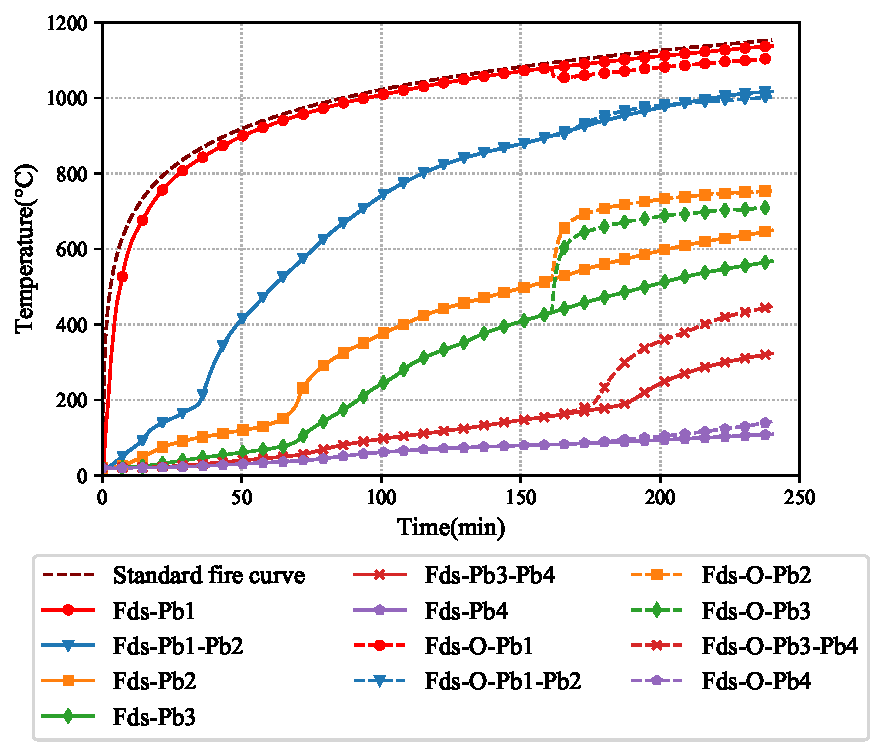
\includegraphics[width=\textwidth]{ST-70-075-2x16-r2-PB.pdf}
		\caption{}
		\label{subfig:ST-70-075-2x16-r2-PB}
	\end{subfigure}
	\begin{subfigure}[b]{0.6\textwidth}
		\centering
		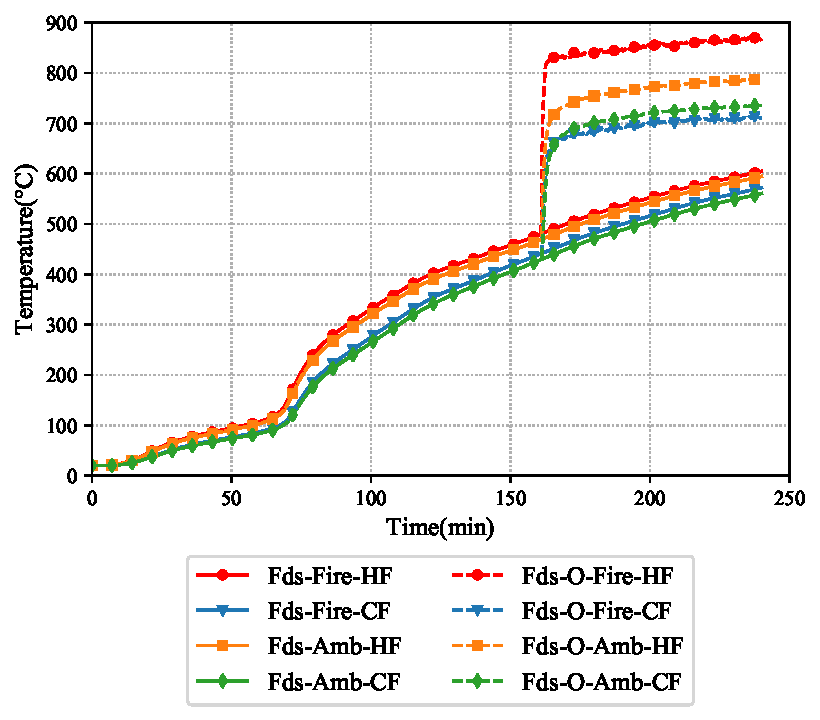
\includegraphics[width=\textwidth]{ST-70-075-2x16-r2-Studs.pdf}
		\caption{}
		\label{subfig:ST-70-075-2x16-r2-Studs}
	\end{subfigure}
	   \caption{Model ST-70-0.75 - Plasterboard and stud time-temperature curves of non-cavity insulated staggered stud wall with 70 $\times$ 0.75 mm studs - (a) Plasterboard temperatures (b) Stud temperatures}
	   \label{fig:ST-70-075-2x16-r2}
\end{figure}

The plasterboard time-temperature curves from non-cavity insulated staggered stud model ST-70-0.75 is shown in \Cref{subfig:ST-70-075-2x16-r2-PB}. All the plasterboard time-temperature curves follow similar pattern till the plasterboard open-up. It is to note that in staggered stud LSF walls the ambient side hot flange (Fds-Amb-HF) is hotter than the fire side cold flange (Fds-Fire-CF). This is because of the staggered stud arrangement within the wall cavity. The ambient side cold flange is located more closer to the fire side plasterboards resulting this behaviour in the stud time-temperature curves. This is also visible on the ambient side hot flange (Fds-O-Amb-HF) of model ST-70-0.75 considering plasterboard open-up as shown in \Cref{subfig:ST-70-075-2x16-r2-Studs}. Also, the temperatures exhibited by the fire and ambient side hot and cold flanges are similar in comparison with each other. In other words, the temperature gradient on the stud flanges in the case of non-cavity insulated staggered stud LSF wall is lesser in comparison with the other wall configurations such as double stud and shaftliner LSF walls. However, the temperature gradient is significant if plasterboard open-up is taken into consideration as shown in \Cref{subfig:ST-70-075-2x16-r2-Studs}.   
\begin{figure}[!htbp]
	\centering
	\begin{subfigure}[b]{0.6\textwidth}
		\centering
		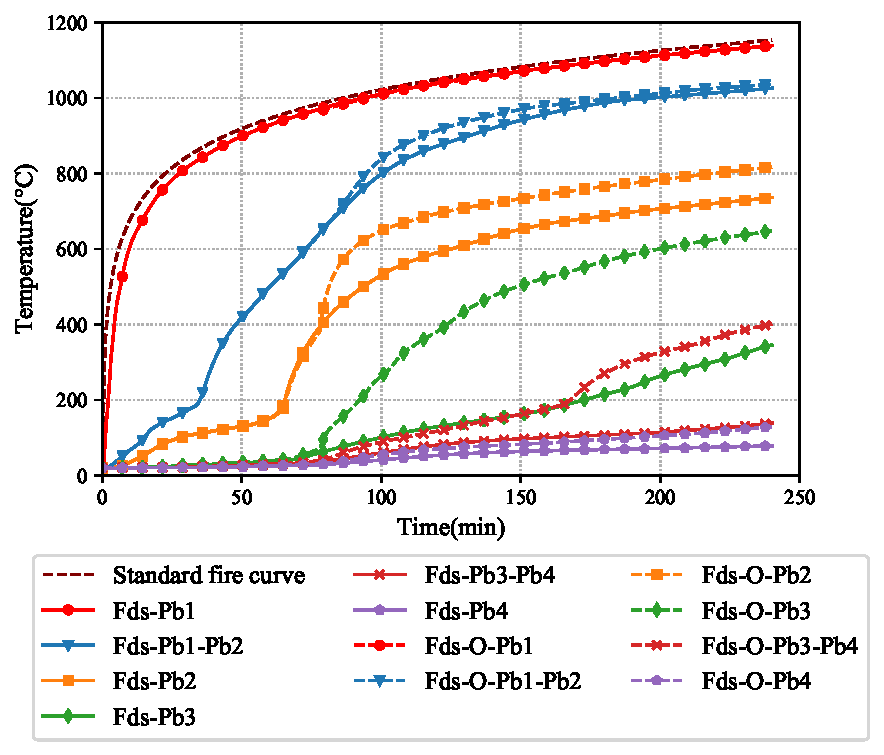
\includegraphics[width=\textwidth]{ST-70-075-2x16-FI-r3-PB.pdf}
		\caption{}
		\label{subfig:ST-70-075-2x16-FI-r3-PB}
	\end{subfigure}
	\begin{subfigure}[b]{0.6\textwidth}
		\centering
		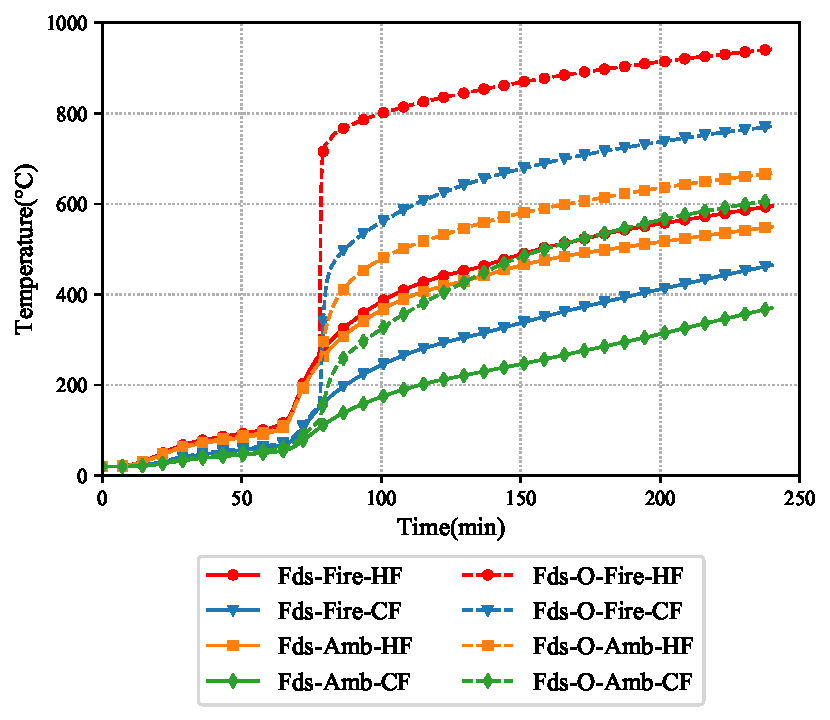
\includegraphics[width=\textwidth]{ST-70-075-2x16-FI-r3-Studs.pdf}
		\caption{}
		\label{subfig:ST-70-075-2x16-FI-r3-Studs}
	\end{subfigure}
	   \caption{Model ST-70-0.75-FI - Plasterboard and stud time-temperature curves of cavity insulated staggered stud wall with 70 $\times$ 0.75 mm studs - (a) Plasterboard temperatures (b) Stud temperatures}
	   \label{fig:ST-70-075-2x16-FI-r3}
\end{figure}

Plasterboard time-temperature curves for staggered stud model with cavity insulation (ST-70-0.75-FI) is shown in \Cref{subfig:ST-70-075-2x16-FI-r3-PB}. The steep increase in the fire side plasterboard interface (Fds-Pb1-Pb2) time-temperature curve happened at a similar time to that of the non-cavity insulated model. This is attributed by the reduced cavity depth of 90 mm used in the model. The ambient side plasterboard curves (Fds and Fds-O-Pb3-Pb4 and Pb4) recorded temperatures less than 200\degree C inferring the absence of insulation failure in the model irrespective of the plasterboard open-up as shown in \Cref{fig:ST-70-075-2x16-FI-r3}. Also, in the cavity insulated model ST-70-0.75-FI with plasterboard open-up the fire side cold flange (Fds-O-Fire-CF) is hotter than the ambient side hot flange (Fds-O-Amb-HF). This is because, in the thermal model, the plasterboard open-up was assumed to occur near the fire side studs causing the temperatures of the flanges to be higher than the ambient side studs where the plasterboard was intact. The cavity insulation entraps the heat on the fire side due to the linear arrangement within the cavity thus causing this time-temperature profile in studs.
\begin{figure}[!htbp]
	\centering
	\begin{subfigure}[b]{0.6\textwidth}
		\centering
		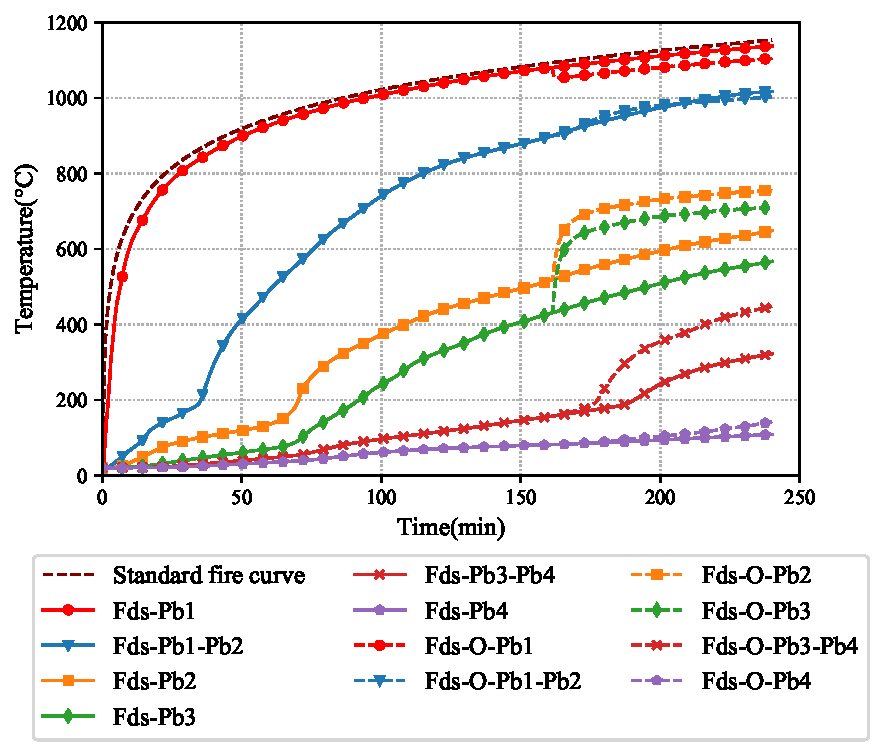
\includegraphics[width=\textwidth]{ST-70-095-2x16-r2-PB.pdf}
		\caption{}
		\label{subfig:ST-70-095-2x16-r2-PB}
	\end{subfigure}
	\begin{subfigure}[b]{0.6\textwidth}
		\centering
		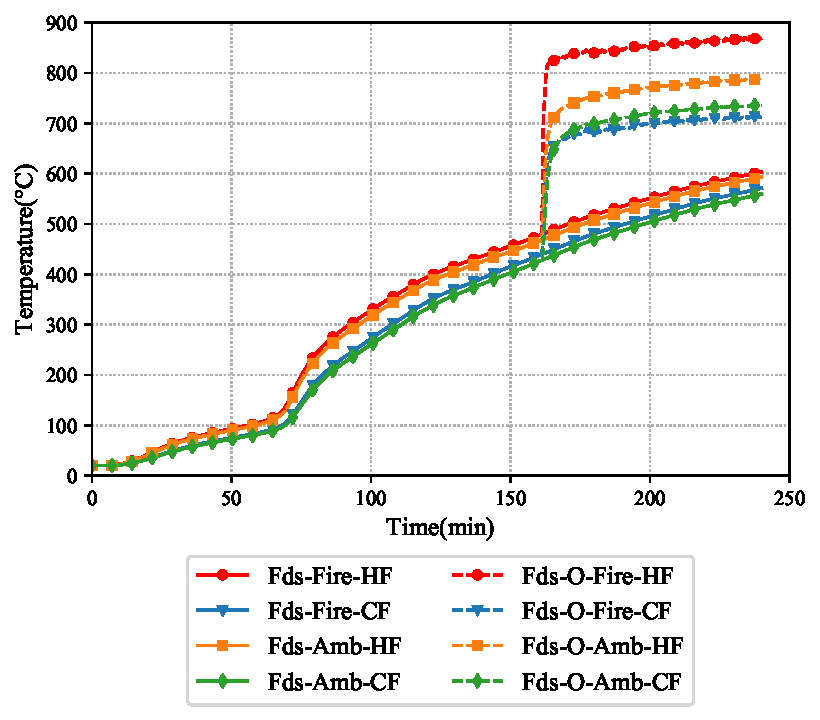
\includegraphics[width=\textwidth]{ST-70-095-2x16-r2-Studs.pdf}
		\caption{}
		\label{subfig:ST-70-095-2x16-r2-Studs}
	\end{subfigure}
	   \caption{Model ST-70-0.95 - Plasterboard and stud time-temperature curves of non-cavity insulated staggered stud wall with 70 $\times$ 0.95 mm studs - (a) Plasterboard temperatures (b) Stud temperatures}
	   \label{fig:ST-70-095-2x16-r2}
\end{figure}
\begin{figure}[!htbp]
	\centering
	\begin{subfigure}[b]{0.6\textwidth}
		\centering
		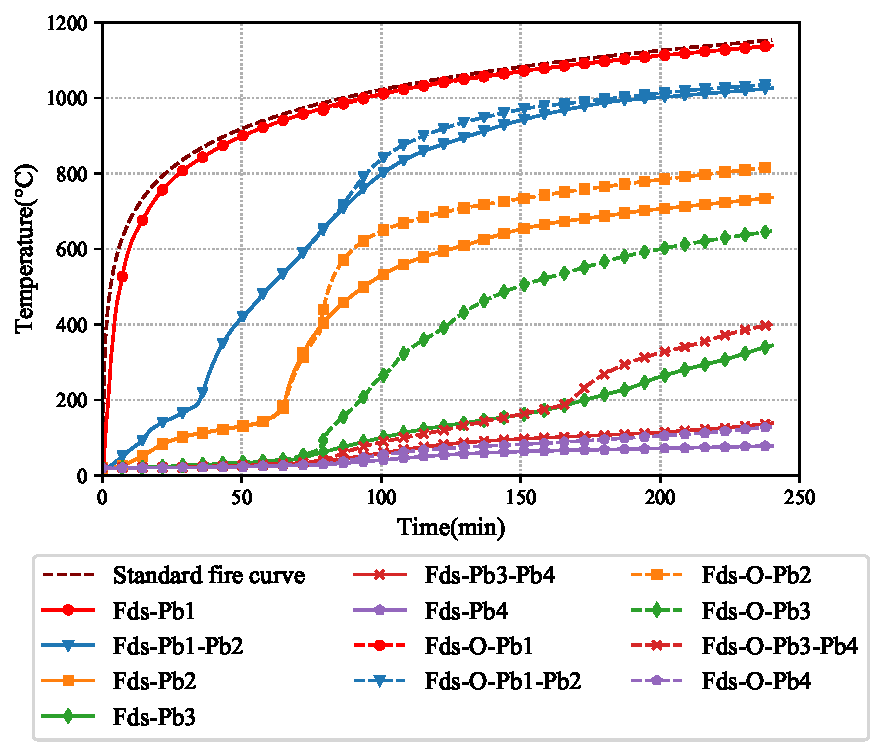
\includegraphics[width=\textwidth]{ST-70-095-2x16-FI-r3-PB.pdf}
		\caption{}
		\label{subfig:ST-70-095-2x16-FI-r3-PB}
	\end{subfigure}
	\begin{subfigure}[b]{0.6\textwidth}
		\centering
		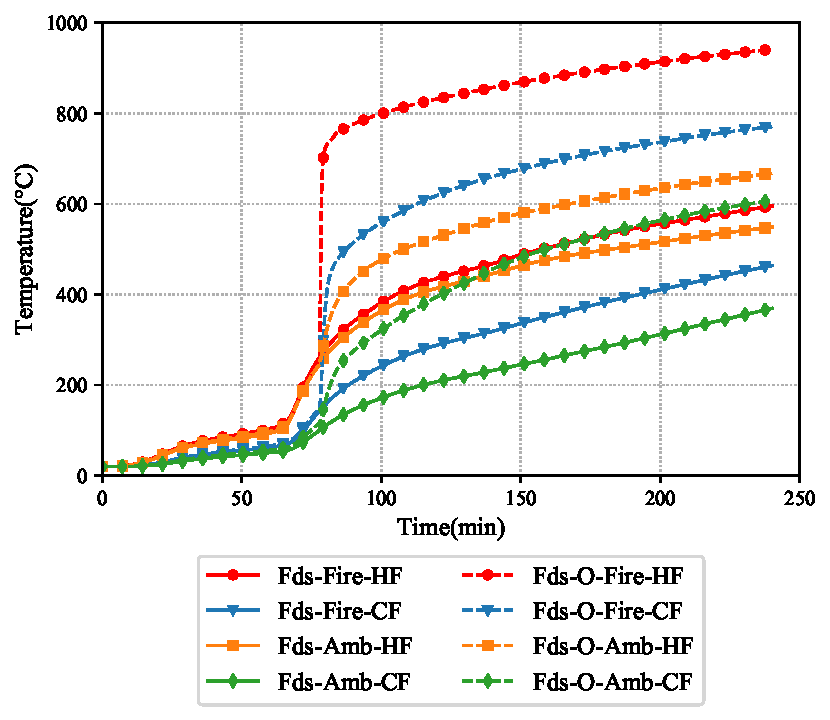
\includegraphics[width=\textwidth]{ST-70-095-2x16-FI-r3-Studs.pdf}
		\caption{}
		\label{subfig:ST-70-095-2x16-FI-r3-Studs}
	\end{subfigure}
	   \caption{Model ST-70-0.95-FI - Plasterboard and stud time-temperature curves of cavity insulated staggered stud wall with 70 $\times$ 0.95 mm studs - (a) Plasterboard temperatures (b) Stud temperatures}
	   \label{fig:ST-70-095-2x16-FI-r3}
\end{figure}

The staggered stud model was continued with 70 $\times$ 0.95 mm studs. Time-temperature curves of stud plasterboard corresponding to non-cavity insulated model ST-70-0.95 is shown in \Cref{fig:ST-70-095-2x16-r2}. The plasterboard and stud time-temperature curves of the model ST-70-0.95 were similar in comparison to the model with 0.75 mm thick studs. The phenomenon of fire side cold flange in stud (Fire-CF) was hotter in comparison with ambient side hot flange (Amb-HF) irrespective of the plasterboard open-up was noticeable in the ST-70-0.95-FI.

\subsection{Staggered stud walls with 90 mm studs}

This section details the thermal model results of staggered stud walls conducted with 90 mm deep studs with 0.75 and 0.95 mm thickness. An effective cavity depth of 150 mm was maintained in the staggered stud model. Unlike the staggered stud model with 70 mm deep studs with linear cavity insulation the staggered stud model with 90 mm deep studs had the cavity insulation staggered around the studs. Non-cavity insulated staggered stud walls with 90 $\times$ 0.75 mm studs and cavity insulated staggered stud wall with 90 $\times$ 0.95 mm studs have already been investigated through experimental methods in \Cref{ch:Fire} and the same has been simulated in \Cref{ch:FE-Thermal} and will not be considered for investigation in this section. The plasterboard interface time-temperature curve (Fds and Fds-O-Pb1-Pb2) exhibited a similar behaviour in the model ST-90-0.75-FI irrespective of the plasterboard open-up. The fire side cavity time-temperature cure in the plasterboard open-up model exhibited a sudden increase in the curve in comparison with the other ambient side time-temperature curves. However, the ambient side plasterboard time-temperature curve was less than 200\degree C in both the thermal model simulation indicating the absence of insulation failure in models.   

Likewise, the plasterboard time-temperature curves of the non-cavity insulated thermal model (ST-90-0.95) with 90 $\times$ 0.95 mm studs are shown in \Cref{subfig:ST-90-095-2x16-r2-PB}. The plasterboard interface time-temperature curve (Fds and Fds-O-Pb1-Pb2) was similar in both the models with and without plasterboard open-up. However, a sudden increase in the fire and ambient side cavity (Fds-O-Pb2 and Pb3) time-temperature curves were noticed in the ST-90-0.95 model considering plasterboard open-up as shown in \Cref{subfig:ST-90-095-2x16-r2-PB}. This might lead to higher temperatures on the ambient side plasterboard. However, similar to other non cavity insulated models the temperatures on the ambient side plasterboards (Fds and Fds-O-Pb) was less than 200\degree C inferring the absence of insulation failure in the model.  
\begin{figure}[!htbp]
	\centering
	\begin{subfigure}[b]{0.6\textwidth}
		\centering
		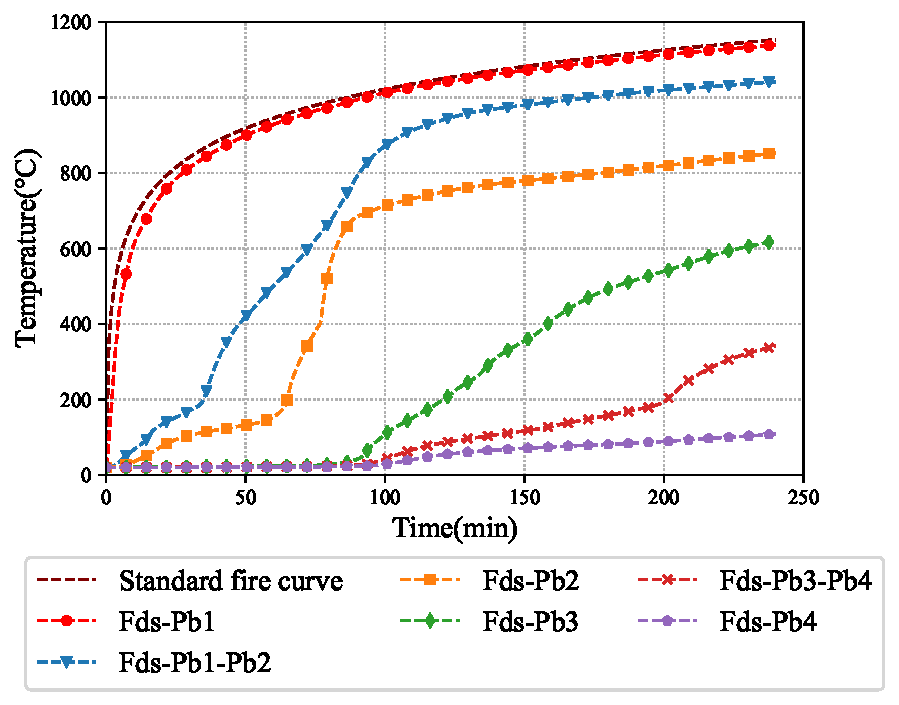
\includegraphics[width=\textwidth]{ST-90-075-2x16-FI-r1-PB.pdf}
		\caption{}
		\label{subfig:ST-90-075-2x16-FI-r1-PB}
	\end{subfigure}
	\begin{subfigure}[b]{0.6\textwidth}
		\centering
		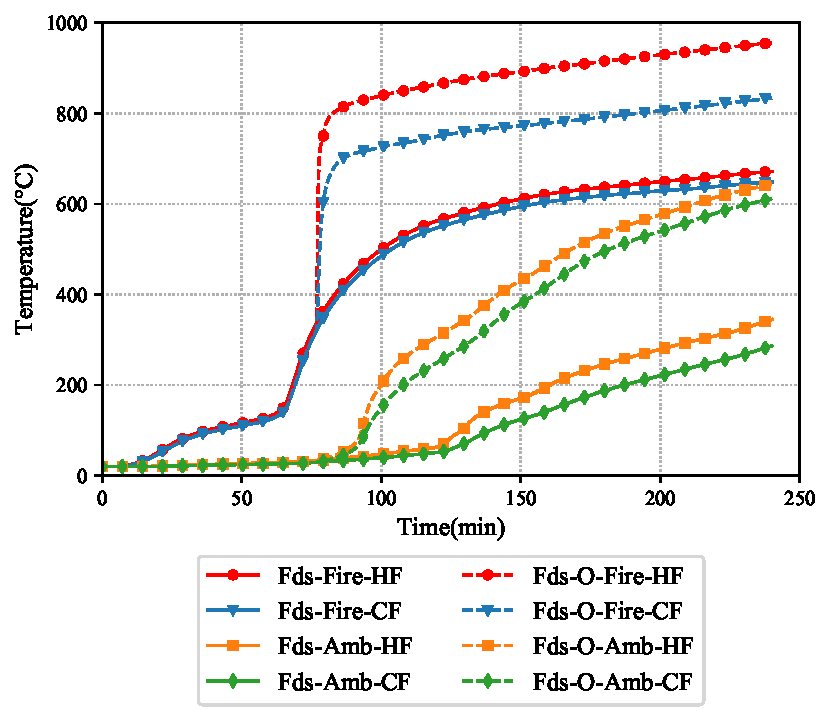
\includegraphics[width=\textwidth]{ST-90-075-2x16-FI-r1-Studs.pdf}
		\caption{}
		\label{subfig:ST-90-075-2x16-FI-r1-Studs}
	\end{subfigure}
	   \caption{Model ST-90-0.75-FI - Plasterboard and stud time-temperature curves of cavity insulated staggered stud wall with 70 $\times$ 0.75 mm studs - (a) Plasterboard temperatures (b) Stud temperatures}
	   \label{fig:ST-90-075-2x16-FI-r1}
\end{figure}
\begin{figure}[!htbp]
	\centering
	\begin{subfigure}[b]{0.6\textwidth}
		\centering
		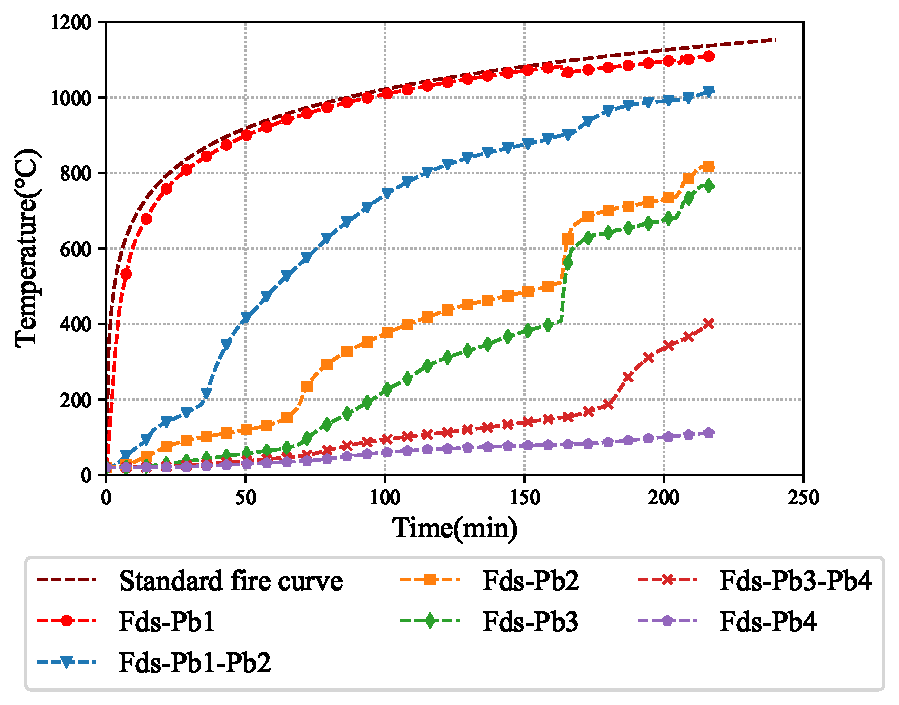
\includegraphics[width=\textwidth]{ST-90-095-2x16-r2-PB.pdf}
		\caption{}
		\label{subfig:ST-90-095-2x16-r2-PB}
	\end{subfigure}
	\begin{subfigure}[b]{0.6\textwidth}
		\centering
		\includegraphics[width=\textwidth]{ST-90-095-2x16-r2-Studs.pdf}
		\caption{}
		\label{subfig:ST-90-095-2x16-r2-Studs}
	\end{subfigure}
	   \caption{Model ST-90-0.95 - Plasterboard and stud time-temperature curves of non-cavity insulated staggered stud wall with 90 $\times$ 0.95 mm studs - (a) Plasterboard temperatures (b) Stud temperatures}
	   \label{fig:ST-90-095-2x16-r2}
\end{figure}

Stud time-temperature curves for the thermal model ST-90-0.75-FI is shown in \Cref{subfig:ST-90-075-2x16-FI-r1-Studs}. The fire side hot and cold flange temperatures (Fds-O-Fire-HF and CF) recorded similar temperatures in the ST-90-0.75-FI model without plasterboard open-up. The gradient in temperature between the fire side hot and cold flanges was minimal in the fire side hot and cold flanges. However, the temperature gradient was smaller in the ambient side hot and cold flanges (Fds-O-Amb-HF and CF) in the model considering the plasterboard open-up. The difference in temperatures between the stud hot and cold flanges of the fire and ambient side in the model ST-90-0.75-FI was higher in models irrespective of the plasterboard open-up. This is attributed by the glass fibre insulation staggered within the cavity entrapping the heat on the fire side of the model. This observation was noticed in all the thermal models with cavity insulation. Stud time-temperature curves for the non-cavity insulated model ST-90-0.95 is shown in \Cref{subfig:ST-90-095-2x16-r2-Studs}. The observations in the stud curves are similar irrespective of the plasterboard open-up and replicated the behaviour observed in staggered stud walls with 70 mm deep studs. This includes the resemblance of the time-temperature curve pattern exhibited by all the  stud flanges. However, the sudden increase in the time-temperature curve of the stud flanges was noticeable in the model with plasterboard open-up due to the direct exposure of heat on the studs.   

\section{Ambient Temperature Structural Models}

To determine the failure time of the selected wall configurations, the ambient temperature axial compression capacity of the studs are essential. Therefore, based on the validated ambient capacity structural FE model in ABAQUS from \Cref{ch:FE-Structural} for the experimental investigations conducted in \Cref{ch:Ambient}, structural models were created and analysed for the selected wall configurations. 3D shell models were created with single stud set and the ambient temperature axial capacity predictions were derived. The structural FE models were created for the wall configurations which include DS-70-0.75, SL-70-0.75, SL-70-0.95, SL-90-0.75, SL-90-0.95, ST-70-0.75, ST-70-0.95, ST-90-0.75 as detailed in \Cref{tab:fds-parametric-models}. The applied axial load versus axial displacement curves from the conducted structural analysis is shown in \Cref{fig:ambient-capacity-parametric}. Failure load of the structural models are detailed in \Cref{tab:ambient-parametric}
\begin{figure}[!htbp]
	\centering
	\begin{subfigure}[b]{0.4\textwidth}
			\centering
		\includegraphics[width=\textwidth]{DS-70-075-2x16-gen-r0.pdf}
		\caption{}
		\label{subfig:DS-70-075-2x16-gen-r0}
	\end{subfigure}
	\begin{subfigure}[b]{0.4\textwidth}
			\centering
		\includegraphics[width=\textwidth]{SL-70-075-2x16-gen-r0.pdf}
		\caption{}
		\label{subfig:SL-70-075-2x16-gen-r0}
	\end{subfigure}
	\begin{subfigure}[b]{0.4\textwidth}
			\centering
		\includegraphics[width=\textwidth]{SL-70-095-2x16-gen-r0.pdf}
		\caption{}
		\label{subfig:SL-70-095-2x16-gen-r0}
	\end{subfigure}
	\begin{subfigure}[b]{0.4\textwidth}
			\centering
		\includegraphics[width=\textwidth]{SL-90-075-2x16-gen-r0.pdf}
		\caption{}
		\label{subfig:SL-90-075-2x16-gen-r0}
	\end{subfigure}
	\begin{subfigure}[b]{0.4\textwidth}
			\centering
		\includegraphics[width=\textwidth]{SL-90-095-2x16-gen-r0.pdf}
		\caption{}
		\label{subfig:SL-90-095-2x16-gen-r0}
	\end{subfigure}
	\begin{subfigure}[b]{0.4\textwidth}
			\centering
		\includegraphics[width=\textwidth]{ST-70-075-2x16-gen-r0.pdf}
		\caption{}
		\label{subfig:ST-70-075-2x16-gen-r0}
	\end{subfigure}
	\begin{subfigure}[b]{0.4\textwidth}
			\centering
		\includegraphics[width=\textwidth]{ST-70-095-2x16-gen-r0.pdf}
		\caption{}
		\label{subfig:ST-70-095-2x16-gen-r0}
	\end{subfigure}
	\begin{subfigure}[b]{0.4\textwidth}
			\centering
		\includegraphics[width=\textwidth]{ST-90-075-2x16-gen-r0.pdf}
		\caption{}
		\label{subfig:ST-90-075-2x16-gen-r0}
	\end{subfigure}
	   \caption{Ambient temperature axial compression capacity of complex LSF walls considered for parametric analysis (a) DS-70-0.75, (b) SL-70-0.75, (c) SL-70-0.95, (d) SL-90-0.75, (e) SL-90-0.95, (f) ST-70-0.75, (g) ST-70-0.95, (h) ST-90-0.75}
	   \label{fig:ambient-capacity-parametric}
\end{figure}

Amongst the selected complex LSF wall configurations, the model SL-90-0.95 resulted in the maximum axial compression capacity of 85.83 kN as shown in \Cref{tab:ambient-parametric}. This is attributed by the slenderness ration of the thick 0.95 mm studs along with the effective lateral restraints provided to both the stud flanges through plasterboards in the case of shaftliner LSF wall configuration. However, it is to note that the staggered stud wall model with 70 $\times$ 0.95 mm studs (ST-70-0.95) resulted in the third highest axial compression capacity of 65.87 kN. Likewise the axial compression capacity of the staggered stud wall model with 70 $\times$ 0.75 mm studs (ST-70-0.75) resulted an axial capacity of 48.03 kN which is higher than the axial compression capacity of the double stud wall model DS-70-0.75 considering the same stud section. However, in the case of double stud wall effective restraints are provided on one flange of the stud. In the case of staggered stud wall effective restraints are provided on the stud flange through plasterboard and on the web service holes through omega nogging. This difference in restraint arrangement might have attributed to the superior axial compression capacity performance in staggered stud LSF walls.
\begin{table}[!htbp]
	\centering
	\begin{threeparttable}
			\caption{Ambient temperature axial compression capacity of FE structural models}
				\begin{tabular}{ccc}
					\toprule
					Model & Description & Failure Load (kN) \\
					\midrule
					DS-70-0.75 & Double stud - 70$\times$0.75 & 47.05 \\
					DS-70-0.95 & Double stud - 70$\times$0.95 (AT4)$^*$ & 71.81 \\
					DS-90-0.75 & Double stud - 90$\times$0.75 (AT2)$^*$ & 46.25 \\
					DS-90-0.95 & Double stud - 90$\times$0.95 (AT1)$^*$ & 71.97 \\
					SL-70-0.75 & Shaftliner - 70$\times$0.75 & 58.81 \\
					SL-70-0.95 & Shaftliner - 70$\times$0.95 & 81.97 \\
					SL-90-0.75 & Shaftliner - 90$\times$0.75 & 55.85 \\
					SL-90-0.95 & Shaftliner - 90$\times$0.95 & 85.83 \\
					ST-70-0.75 & Staggered stud - 70$\times$0.75 & 48.03 \\
					ST-70-0.95 & Staggered stud - 70$\times$0.95 & 65.87 \\
					ST-90-0.75 & Staggered stud - 90$\times$0.75 & 40.9 \\
					ST-90-0.95 & Staggered stud - 90$\times$0.95 (AT5)$^*$ & 60.98 \\
					\bottomrule
				\end{tabular}%
					\label{tab:ambient-parametric}%
						\begin{tablenotes}
							\small
							\item \textit{\(^*\) FE model predictions from \Cref{ch:FE-Structural}, \Cref{tab:ambient-test-results-fea}}
						\end{tablenotes}
	\end{threeparttable}
\end{table}% 

To understand the behaviour of the complex LSF wall configurations further under ambient temperature, investigation was conducted by comparing the structural FE model results of the experimental investigation from \Cref{ch:FE-Structural} with the results from parametric FE model configurations. Comparison of the axial compression capacity in terms of applied axial load versus axial displacement curves between the experimental model from \Cref{ch:FE-Structural} and results from the models considered for the parametric study are presented in \Cref{fig:ambient-parametric}.

\begin{figure}[!htbp]
	\centering
	\includegraphics[scale=0.8]{ambient-parametric.pdf}
	\caption{Comparison of axial compression capacity from experimental and parametric FE model}
	\label{fig:ambient-parametric}
\end{figure}

Comparison of the ambient temperature axial load carrying capacity from FE model shows that the shaftliner model SL-90-0.95 resulted in the maximum capacity of 85.83 kN in comparison with other models. This is attributed by the lateral restraint on both the stud flanges. However, the double stud model resulted in a capacity of 71.97 kN and the staggered stud model resulted in a capacity of 60.98 kN with the same stud geometry of 90 $\times$ 0.95. But in the case of complex wall configurations with 70 $\times$ 0.75 mm studs the staggered stud wall model ST-70-0.75 resulted a higher capacity of 48.03 kN in comparison with the double stud wall model DS-70-0.75 resulting 47.05 kN. This infers that, the staggered stud wall with 70 $\times$ 0.75 mm studs performs better in comparison with a similar double stud wall. 

It is to note that, for a double stud wall with 70 mm deep studs the effective cavity width will be 160 mm while it is 90 mm in the case of staggered stud wall. This might result in considerable savings in the floor space in a building. Also, no wall configuration with 0.75 mm thick studs resulted in higher axial compression load in comparison with the 0.95 mm thick stud wall configurations. If the floor space in a building is considered as the governing criteria, staggered stud wall with 70 $\times$ 0.95 mm studs (ST-70-0.95) would be the optimal choice under load bearing condition based on the conducted parametric investigation under ambient temperature conditions. However, performance of these walls under fire conditions needs further investigation and are discussed next.  

\section{Elevated Temperature Structural Models}

To determine the failure time of the selected wall configuration in the parametric study under fire conditions, sequentially coupled temperature displacement analysis was conducted under different load ratios (LR's). Typically, the design load on the LSF wall varies between 20\% to 70\% of the ambient temperature axial compression capacity of the wall. Therefore, the parametric study was limited to determine the FRL of the selected LSF wall configurations within 0.2 to 0.7 LR. The ambient capacity detailed in \Cref{tab:ambient-parametric} was used to determine the loads corresponding to the required LR. Procedure for the coupled temperature displacement structural analysis was similar to those detailed in \Cref{ch:FE-Structural}, \Cref{sec:temp-disp-structural}. Sequentially coupled temperature displacement analysis was conducted in ABAQUS for all the configurations listed in \Cref{tab:fds-parametric-models}. 

\subsection[FRL Predictions for Configurations from Experimental Study]{FRL Predictions for Configurations \\from Experimental Study}

This section details the failure time and corresponding FRL rounded to the nearest 60 min for configurations considered in the experimental study in \Cref{ch:Fire}, \Cref{sec:fire-test-panel-details}, \Cref{tab:test-specimens}. The failure time for the corresponding load ratio from 0.2 to 0.7 is detailed as load ratio versus failure time curves while the corresponding FRL is given in tables to represent the FRL in min for the structural adequacy criteria. As per the National Construction Code of Australia (\citet{ncc2019}) the minimum FRL required for the complex LSF walls used as internal partitions should satisfy a minimum structural integrity criteria of 60 min when exposed to fire. Therefore, the FE models which resulted in a structural failure time of 60 min was taken for investigation irrespective of the applied load ratio and is represented as 60/-/-. Likewise, models which did not satisfy this criteria were given a neutral FRL and is represented as -/-/-.   
\begin{figure}[!htbp]
	\centering
	\includegraphics[scale=0.6]{frl-experiment.pdf}
	\caption{FRL of LSF wall configurations from experimental study}
	\label{fig:frl-experiment}
\end{figure}

The FRL of the configurations considered for the experimental investigation from 0.2 to 0.7 load ratios are shown in \Cref{fig:frl-experiment} and is also detailed in \Cref{tab:frl-parametric-experiment}. The FRL of the considered wall configurations were determined by conducting sequentially coupled temperature-displacement analysis based on the stud temperatures from the FDS thermal models from \Cref{sec:fds-cavity-models,sec:thermal-model-non-cav} of \Cref{ch:FE-Thermal}. This includes the double stud, staggered stud and shaftliner LSF walls configurations conducted as Tests-T1 to T10. 
\begin{table}[!htbp]
	\centering
	\caption{FRL from parametric study on double stud walls with 70 mm deep studs}
	  \begin{tabular}{cccc}
	  \toprule
	  Configuration & LR    & Failure Time (min) & FRL \\
	  \midrule
	  \multirow{6}[2]{*}{DS-70-0.95} & 0.2   & 240   & 240/-/- \\
			& 0.3   & 240   & 240/-/- \\
			& 0.4   & 178.36 & 120/-/- \\
			& 0.5   & 125.33 & 60/-/- \\
			& 0.6   & 124.62 & 90/-/- \\
			& 0.7   & 82.37 & 60/-/- \\
	  \midrule
	  \multirow{6}[2]{*}{DS-90-0.75} & 0.2   & 240   & 240/-/- \\
			& 0.3   & 240   & 240/-/- \\
			& 0.4   & 174.32 & 120/-/- \\
			& 0.5   & 170   & 120/-/- \\
			& 0.6   & 82    & 60/-/- \\
			& 0.7   & 82    & 60/-/- \\
	  \midrule
	  \multirow{6}[2]{*}{DS-90-0.95} & 0.2   & 240   & 240/-/- \\
			& 0.3   & 240   & 240/-/- \\
			& 0.4   & 174.83 & 120/-/- \\
			& 0.5   & 174.36 & 120/-/- \\
			& 0.6   & 142.89 & 120/-/- \\
			& 0.7   & 87.33 & 60/-/- \\
	  \midrule
	  \multirow{6}[2]{*}{DS-90-0.95-AI} & 0.2   & 84.88 & 60/-/- \\
			& 0.3   & 81.78 & 60/-/- \\
			& 0.4   & 81.6  & 60/-/- \\
			& 0.5   & 81.56 & 60/-/- \\
			& 0.6   & 81.49 & 60/-/- \\
			& 0.7   & 81.33 & 60/-/- \\
	  \midrule
	  \multirow{6}[2]{*}{DS-90-0.95-BI} & 0.2   & 90.21 & 90/-/- \\
			& 0.3   & 79.91 & 60/-/- \\
			& 0.4   & 79.63 & 60/-/- \\
			& 0.5   & 79.61 & 60/-/- \\
			& 0.6   & 79.36 & 60/-/- \\
			& 0.7   & 79.33 & 60/-/- \\
	  \midrule
	  \multirow{6}[2]{*}{SL-90-0.75} & 0.2   & 118.68 & 90/-/- \\
			& 0.3   & 105.55 & 90/-/- \\
			& 0.4   & 103.84 & 90/-/- \\
			& 0.5   & *     & * \\
			& 0.6   & *     & * \\
			& 0.7   & *     & * \\
	  \bottomrule
	\end{tabular}%
  \label{tab:frl-parametric-experiment-a}%
\end{table}%
\begin{table}[htbp]
	\ContinuedFloat
	\centering
	\caption{Continued...}
	  \begin{tabular}{cccc}
	  \toprule
	  Configuration & LR    & Failure Time (min) & FRL \\
	  \midrule
	  \multirow{6}[2]{*}{ST-90-075-2x16} & 0.2   & 164.25 & 120/-/- \\
			& 0.3   & 164.18 & 120/-/- \\
			& 0.4   & 152.53 & 120/-/- \\
			& 0.5   & 123.16 & 120/-/- \\
			& 0.6   & 92.5  & 90/-/- \\
			& 0.7   & *     & * \\
	  \midrule
	  \multirow{6}[2]{*}{ST-90-095-2x16-FI} & 0.2   & 116.45 & 90/-/- \\
			& 0.3   & 100.35 & 90/-/- \\
			& 0.4   & 92.97 & 90/-/- \\
			& 0.5   & 77.5  & 60/-/- \\
			& 0.6   & 77    & 60/-/- \\
			& 0.7   & *     & * \\
	  \bottomrule
	  \end{tabular}%
	\label{tab:frl-parametric-experiment}%
  \end{table}%
  
The FRL of the non-cavity insulated double stud walls (DS-70-095-2x16, DS-90-075-2x16 and DS-90-095-2x16) resulted an FRL of 240 min up to 0.3 LR. However, the maximum FRL achieved by the cavity insulated double stud walls (DS-90-095-2x16-AI, DS-90-095-2x16-BI) was 90 min. This is in correlation with the experimental findings from \Cref{ch:Fire}. The non-cavity insulated shaftliner LSF wall (SL-90-075-2x16) resulted an FRL of 90 min for 0.2 to 0.4 LR. However, due to sever numerical instabilities causing convergence issues in the FE model the FRL of the shaftliner wall SL-90-075-2x16 above 0.4 LR could not be determined. But it can be inferred that the FRL beyond 0.4 LR could not be higher than 90 min based on the FRL predictions up to 90 min. The non-cavity insulated staggered stud wall configuration (ST-90-075-2x16) resulted an FRL of 120 min for LR 0.2 to 0.5. However, the FRL was reduced to 90 min for configuration ST-90-075-2x16 under 0.6 LR. The FRL of the configuration ST-90-075-2x16 under 0.7 LR could not be determined due to convergence issues with the FE model. From the non-cavity insulated wall configurations considered in this section the double stud wall with 90 $\times$ 0.95 mm studs (DS-90-095-2x16) performed better even under high load ratios of 0.6 LR. In the case of cavity insulated walls the staggered stud wall with 90 $\times$ 0.95 mm studs (ST-90-095-2x16-FI) performed better till 0.5 LR. As plasterboard open-up was considered in the thermal analysis, the stud hot flange temperatures rapidly increases at the open up time in the complex LSF wall configurations. The fire side hot flange temperatures governs the structural failure in load bearing LSF walls. Therefore, this sudden increase in the temperatures will result in similar failure times of the LSF wall irrespective of the load ratio. Further wall configurations considered in the parametric study are discussed next.

\subsection{FRL Predictions for Configurations from Parametric Study}

This section presents the FRL of all the configurations considered for the parametric study in this research. Twelve double stud wall, eight shaftliner wall and eight staggered stud wall configurations were considered for the parametric study. Each wall configuration was analysed for load ratios from 0.2 to 0.7 accounting to 168 FE structural models. The parameters included 70 and 90 mm deep studs with 0.75 and 0.95 mm thicknessess corresponding to the configurations considered in the parametric thermal analysis. This also includes non-cavity insulated and cavity insulated wall configurations.

\subsubsection{FRL Predictions of Double Stud LSF Wall Configurations}

The double stud LSF wall configurations considered for the parametric analysis are discussed in this section. \Cref{fig:frl-DS-parametric} shows the load ratio versus time scattered plots for the considered double stud LSF wall configurations. The FRLs of the double stud wall configurations are presented in \Cref{tab:frl-parametric-ds-70}. 
\begin{figure}[!htbp]
	\centering
	\includegraphics[scale=0.6]{frl-DS-parametric.pdf}
	\caption{FRL of double stud wall configurations from parametric study}
	\label{fig:frl-DS-parametric}
\end{figure}
% Table generated by Excel2LaTeX from sheet 'DS-70'
\begin{table}[!htbp]
	\centering
	\caption{FRL of double stud walls with 70 mm deep studs}
	  \begin{tabular}{cccc}
	  \toprule
	  Configuration & LR    & Failure Time (min) & FRL \\
	  \midrule
	  \multirow{6}[2]{*}{DS-70-0.75} & 0.2   & 178.38 & 120/-/- \\
			& 0.3   & 178.4 & 120/-/- \\
			& 0.4   & 178.31 & 120/-/- \\
			& 0.5   & *     & * \\
			& 0.6   & 110.69 & 90/-/- \\
			& 0.7   & 82.36 & 60/-/- \\
	  \midrule
	  \multirow{6}[2]{*}{DS-70-0.75-AI} & 0.2   & 80.9  & 60/-/- \\
			& 0.3   & 80.9  & 60/-/- \\
			& 0.4   & 80.65 & 60/-/- \\
			& 0.5   & 80.38 & 60/-/- \\
			& 0.6   & 80.15 & 60/-/- \\
			& 0.7   & 74.97 & 60/-/- \\
	  \midrule
	  \multirow{6}[2]{*}{DS-70-0.75-BI} & 0.2   & 79.18 & 60/-/- \\
			& 0.3   & 79.16 & 60/-/- \\
			& 0.4   & 78.83 & 60/-/- \\
			& 0.5   & 78.43 & 60/-/- \\
			& 0.6   & 78.04 & 60/-/- \\
			& 0.7   & 71.67 & 60/-/- \\
	  \midrule
	  \multirow{6}[2]{*}{DS-70-0.95} & 0.2   & 240   & 240/-/- \\
			& 0.3   & 240   & 240/-/- \\
			& 0.4   & 178.36 & 120/-/- \\
			& 0.5   & 125.33 & 120/-/- \\
			& 0.6   & 124.62 & 120/-/- \\
			& 0.7   & 82.37 & 60/-/- \\
	  \midrule
	  \multirow{6}[2]{*}{DS-70-0.95-AI} & 0.2   & 82.51 & 60/-/- \\
			& 0.3   & 81.4  & 60/-/- \\
			& 0.4   & 80.87 & 60/-/- \\
			& 0.5   & 80.48 & 60/-/- \\
			& 0.6   & 80.21 & 60/-/- \\
			& 0.7   & 74.52 & 60/-/- \\
	  \midrule
	  \multirow{6}[2]{*}{DS-70-0.95-BI} & 0.2   & 79.9  & 60/-/- \\
			& 0.3   & 79.56 & 60/-/- \\
			& 0.4   & 79.19 & 60/-/- \\
			& 0.5   & 78.64 & 60/-/- \\
			& 0.6   & 77.92 & 60/-/- \\
			& 0.7   & 71.72 & 60/-/- \\
	  \bottomrule
	  \end{tabular}%
	\label{tab:frl-parametric-ds-70}%

	\small \textit{$*$ Model with convergence issues}
  \end{table}%
     
The stud time-temperature curves from the thermal models of double stud wall configurations were extracted from \Cref{sec:ds-70-thermal-fds} and coupled temperature-displacement analysis was conducted. The non-cavity insulated double stud LSF wall with 70 $\times$ 0.95 mm stud (DS-70-095) resulted in the highest FRL of 240 min for 0.2 and 0.3 LR. However, the same non-cavity insulated double stud wall configuration resulted in an FRL of 120 min as shown in \Cref{tab:frl-parametric-ds-70}. This is because of the thinner stud sections used in the model (DS-70-0.95). The model DS-70-0.75 under 0.5 LR suffered convergence issue and the corresponding FRL could not be predicted. The double stud models with cavity insulation resulted an FRL of 60 irrespective of the position of the cavity insulation in all load ratios. This is because of the heat entrapment in the fire side studs experienced by the test wall in \Cref{ch:Fire} resulting in premature failure. 
% Table generated by Excel2LaTeX from sheet 'DS-90'
\begin{table}[!htbp]
	\centering
	\caption{FRL of double stud walls with 90 mm deep studs}
	  \begin{tabular}{cccc}
	  \toprule
	  Configuration & LR    & Failure Time (min) & FRL \\
	  \midrule
	  \multirow{6}[2]{*}{DS-90-0.75} & 0.2   & 240   & 240/-/- \\
			& 0.3   & 240   & 240/-/- \\
			& 0.4   & 174.32 & 120/-/- \\
			& 0.5   & 170   & 120/-/- \\
			& 0.6   & 82    & 60/-/- \\
			& 0.7   & 82    & 60/-/- \\
	  \midrule
	  \multirow{6}[2]{*}{DS-90-0.75-AI} & 0.2   & 84.5  & 60/-/- \\
			& 0.3   & 81.58 & 60/-/- \\
			& 0.4   & 81.15 & 60/-/- \\
			& 0.5   & 81.07 & 60/-/- \\
			& 0.6   & 81    & 60/-/- \\
			& 0.7   & 80.33 & 60/-/- \\
	  \midrule
	  \multirow{6}[2]{*}{DS-90-0.75-BI} & 0.2   & * & * \\
			& 0.3   & 79.79 & 60/-/- \\
			& 0.4   & 79.35 & 60/-/- \\
			& 0.5   & 79.34 & 60/-/- \\
			& 0.6   & 79.16 & 60/-/- \\
			& 0.7   & 78.66 & 60/-/- \\
	  \midrule
	  \multirow{6}[2]{*}{DS-90-0.95} & 0.2   & 240   & 240/-/- \\
			& 0.3   & 240   & 240/-/- \\
			& 0.4   & 174.83 & 120/-/- \\
			& 0.5   & 174.36 & 120/-/- \\
			& 0.6   & 142.89 & 120/-/- \\
			& 0.7   & 87.33 & 60/-/- \\
	  \midrule
	  \multirow{6}[2]{*}{DS-90-0.95-AI} & 0.2   & 84.88 & 60/-/- \\
			& 0.3   & 81.78 & 60/-/- \\
			& 0.4   & 81.6  & 60/-/- \\
			& 0.5   & 81.56 & 60/-/- \\
			& 0.6   & 81.49 & 60/-/- \\
			& 0.7   & 81.33 & 60/-/- \\
	  \midrule
	  \multirow{6}[2]{*}{DS-90-0.95-BI} & 0.2   & 90.21 & 90/-/- \\
			& 0.3   & 79.91 & 60/-/- \\
			& 0.4   & 79.63 & 60/-/- \\
			& 0.5   & 79.61 & 60/-/- \\
			& 0.6   & 79.36 & 60/-/- \\
			& 0.7   & 79.33 & 60/-/- \\
	  \bottomrule
	  \end{tabular}%
	\label{tab:frl-parametric-ds-90}%

	\small \textit{$*$ Model with convergence issues}
  \end{table}%

The FRL of double stud walls with 90 mm studs are shown in \Cref{tab:frl-parametric-ds-90}. Similar to the non-cavity double stud walls with 70 mm deep studs the non-cavity insulated double stud wall with 90 $\times$ 0.95 mm (DS-90-0.95) studs resulted in the highest FRL of 240 min for load rations 0.2 and 0.3. The DS-90-0.95 wall could result an FRL of 120 min even under a higher LR of 0.6 while a similar configuration with 0.75 mm (DS-90-0.75) studs resulted an FRL of 60 min. The model DS-90-0.75-BI under 0.2 LR suffered convergence issues and the FRL could not be predicted. Based on the predicted FRLs it can be inferred that the thickness of the studs significantly influence the FRL of double stud LSF walls. When the applied axial load is non-dimensionalised to load ratio the effect of cavity depth do not significantly affect the FRL, however has a moderate influence on the failure time of the test wall. As the FRLs are rounded to the nearest 30 min, the influence of cavity depth on the failure time of the double stud LSF walls can be neglected. 

\subsubsection{FRL Predictions of Shaftliner LSF Wall Configurations}

\begin{figure}[!htbp]
	\centering
	\includegraphics[scale=0.6]{frl-SL-parametric.pdf}
	\caption{FRL of shaftliner wall configurations from parametric study}
	\label{fig:frl-SL-parametric}
\end{figure}
% Table generated by Excel2LaTeX from sheet 'SL-70'
\begin{table}[!htbp]
	\centering
	\caption{FRL of shaftliner walls with 70 mm deep studs}
	  \begin{tabular}{cccc}
	  \toprule
	  Configuration & LR    & Failure Time (min) & FRL \\
	  \midrule
	  \multirow{6}[2]{*}{SL-70-0.75} & 0.2   & 127.17 & 120/-/- \\
			& 0.3   & 126.67 & 120/-/- \\
			& 0.4   & 101.12 & 90/-/- \\
			& 0.5   & 82.78 & 60/-/- \\
			& 0.6   & 73.6  & 60/-/- \\
			& 0.7   & 66.66 & 60/-/- \\
	  \midrule
	  \multirow{6}[2]{*}{SL-70-0.75-FI} & 0.2   & 79.6  & 60/-/- \\
			& 0.3   & 79.09 & 60/-/- \\
			& 0.4   & 78.38 & 60/-/- \\
			& 0.5   & 75.62 & 60/-/- \\
			& 0.6   & 69.98 & 60/-/- \\
			& 0.7   & 52    & - \\
	  \midrule
	  \multirow{6}[2]{*}{SL-70-0.95} & 0.2   & 142.22 & 120/-/- \\
			& 0.3   & 133.52 & 120/-/- \\
			& 0.4   & 106.46 & 90/-/- \\
			& 0.5   & 84.9  & 60/-/- \\
			& 0.6   & 74.53 & 60/-/- \\
			& 0.7   & 63.41 & 60/-/- \\
	  \midrule
	  \multirow{6}[2]{*}{SL-70-0.95-FI} & 0.2   & 81.96 & 60/-/- \\
			& 0.3   & 79.88 & 60/-/- \\
			& 0.4   & 78.64 & 60/-/- \\
			& 0.5   & 77    & 60/-/- \\
			& 0.6   & 70.61 & 60/-/- \\
			& 0.7   & 51    & - \\
	  \bottomrule
	  \end{tabular}%
	\label{tab:frl-parametric-sl-70}%
  \end{table}%

FRLs predictions of the shaftliner LSF walls considered for the parametric analysis are presented in this section. \Cref{fig:frl-SL-parametric} shows the load ratio versus failure time scattered plots. The shaftliner walls were also modelled with 70 and 90 mm deep studs with 0.75 and 0.95 thickness. In the case of cavity insulated shaftliner walls, the cavity insulation was positioned throughout the cavity. The model with ambient side cavity insulation was not considered for investigation. This is because from the experimental investigations conducted in \Cref{ch:Fire} it was found that the position of cavity insulation did not significantly influence the thermal behaviour as the heat entrapment occurred in the walls with ambient side cavity insulation also. This was evident in the FDS thermal models investigated in \Cref{sec:thermal-parametric-models} of this chapter.
% Table generated by Excel2LaTeX from sheet 'SL-90'
\begin{table}[!htbp]
	\centering
	\caption{FRL of shaftliner walls with 90 mm deep studs}
	  \begin{tabular}{cccc}
	  \toprule
	  Configuration & LR    & Failure Time (min) & FRL \\
	  \midrule
	  \multirow{6}[2]{*}{SL-90-0.75} & 0.2   & 118.68 & 90/-/- \\
			& 0.3   & 105.55 & 90/-/- \\
			& 0.4   & 103.84 & 90/-/- \\
			& 0.5   & *     & * \\
			& 0.6   & *     & * \\
			& 0.7   & *     & * \\
	  \midrule
	  \multirow{6}[2]{*}{SL-90-0.75-FI} & 0.2   & 84.4  & 60/-/- \\
			& 0.3   & 80.37 & 60/-/- \\
			& 0.4   & 79.71 & 60/-/- \\
			& 0.5   & 79.16 & 60/-/- \\
			& 0.6   & *     & * \\
			& 0.7   & *     & * \\
	  \midrule
	  \multirow{6}[2]{*}{SL-90-0.95} & 0.2   & 126.5 & 120/-/- \\
			& 0.3   & 121.12 & 120/-/- \\
			& 0.4   & 115.86 & 90/-/- \\
			& 0.5   & 109.2 & 90/-/- \\
			& 0.6   & 71    & 60/-/- \\
			& 0.7   & *     & * \\
	  \midrule
	  \multirow{6}[2]{*}{SL-90-0.95-FI} & 0.2   & 87.44 & 60/-/- \\
			& 0.3   & 80.2  & 60/-/- \\
			& 0.4   & 80    & 60/-/- \\
			& 0.5   & 79.36 & 60/-/- \\
			& 0.6   & 78.16 & 60/-/- \\
			& 0.7   & *     & * \\
	  \bottomrule
	  \end{tabular}%
	\label{tab:frl-parametric-sl-90}%

	\small \textit{$*$ Model with convergence issues}
  \end{table}%

FRLs from shaftliner LSF walls with 70 $\times$ 0.75 and 0.95 studs are shown in \Cref{tab:frl-parametric-sl-70}. Despite separating the cavity into two with the middle plasterboard layer the 70 mm deep shaftliner walls with 0.75 mm and 0.95 mm thick studs could not result an FRL of 240 min under any load ratio. This is attributed by the plasterboard open-up which acts as a critical influencing factor in the stud time-temperature curves which greatly influences the FRL. Due to the presence of middle plasterboard layer, there arises very less cooling affect within the cavity and the stud temperatures are more in comparison with the double stud walls. Despite having plasterboard restraints on both the stud flanges, due to the high temperatures on the stud hot and cold flanges, the shaftliner LSF walls could not perform better in comparison with the double stud walls with 70 mm deep studs. From this it is inferred that the contact between the stud flanges and the plasterboard influences the stud time-temperature curves, thereby affecting the FRL. In the case of cavity insulated walls the heat entrapment was more in comparison with double stud LSF walls with both cavity insulated. This results in a larger temperature gradient between the stud hot and cold flanges. This had attributed to the early failure times resulting in lower FRLs in cavity insulated shaftliner LSF walls. 

FRLs of Shaftliner LSF walls with 90 mm $\times$ 0.75 and 0.95 studs are presented in \Cref{tab:frl-parametric-sl-90}. Due to sever non-linearity resulting in convergence issues some of the FRLs of shaftliner wall with 90 mm deep studs could not be determined and are also shown in \Cref{tab:frl-parametric-sl-90}. Similar to shaftliner LSF walls with 70 mm deep studs, the shaftliner liner LSF walls with 90 mm deep studs could not result an FRL of 240 min for any load ratio irrespective of the thickness of the studs. Also, the maximum FRL achieved by the 90 mm deep shaftliner LSF walls was 120 min from shaftliner wall model with 90 $\times$ 0.95 mm stud (SL-90-095-2x16) under 0.2 and 0.3 LR. This was lower than 120 min from the shaftliner LSF walls with 70 mm studs. This is attributed to the slenderness of the studs and partly due to the heat entrapment on the fire side cavity causing the stud hot flanges to absorb more heat in comparison with the other flanges, thereby resulting in large temperature gradient. The larger temperature gradients have significant influence of the FRLs under load bearing conditions. 

\subsubsection{FRL Predictions of Staggered Stud LSF Wall Configurations}

Parametric study conducted on staggered stud LSF wall models are discussed in this section. The load ratio versus failure time scattered plots for all the considered staggered stud wall configuration is shown in \Cref{fig:frl-ST-parametric}. \Cref{tab:frl-parametric-st-70} presents the details of FRLs of staggered stud LSF wall conducted on 70 mm $\times$ 0.75 and 0.95 mm studs. The maximum FRL achieved by the staggered stud LSF walls with 70 mm deep studs was 120 min. This is attributed to the lateral restraint conditions provided to the studs in the model. As discussed earlier in \Cref{ch:FE-Structural} the staggered stud wall studs are effectively restrained on one flange. 
\begin{figure}[!htbp]
	\centering
	\includegraphics[scale=0.6]{frl-ST-parametric.pdf}
	\caption{FRL of staggered stud wall configurations from parametric study}
	\label{fig:frl-ST-parametric}
\end{figure}
% Table generated by Excel2LaTeX from sheet 'ST-70'
\begin{table}[!htbp]
	\centering
	\caption{FRL of staggered stud walls with 70 mm deep studs}
	  \begin{tabular}{cccc}
	  \toprule
	  Configuration & LR    & Failure Time (min) & FRL \\
	  \midrule
	  \multirow{6}[2]{*}{ST-70-0.75} & 0.2   & 161.49 & 120/-/- \\
			& 0.3   & 125.53 & 120/-/- \\
			& 0.4   & 80.86 & 60/-/- \\
			& 0.5   & 68.46 & 60/-/- \\
			& 0.6   & 19.6  & - \\
			& 0.7   & -     & - \\
	  \midrule
	  \multirow{6}[2]{*}{ST-70-0.75-FI} & 0.2   & 78.69 & 60/-/- \\
			& 0.3   & 78.28 & 60/-/- \\
			& 0.4   & 69.67 & 60/-/- \\
			& 0.5   & 44.44 & - \\
			& 0.6   & 15.54 & - \\
			& 0.7   & 0.8274 & - \\
	  \midrule
	  \multirow{6}[2]{*}{ST-70-0.95} & 0.2   & 147.19 & 120/-/- \\
			& 0.3   & 89.87 & 60/-/- \\
			& 0.4   & 69.18 & 60/-/- \\
			& 0.5   & 17.16 & - \\
			& 0.6   & -     & - \\
			& 0.7   & -     & - \\
	  \midrule
	  \multirow{6}[2]{*}{ST-70-0.95-FI} & 0.2   & 78.76 & 60/-/- \\
			& 0.3   & 78.29 & 60/-/- \\
			& 0.4   & 69.63 & 60/-/- \\
			& 0.5   & 33.18 & - \\
			& 0.6   & 12.91 & - \\
			& 0.7   & -     & - \\
	  \bottomrule
	  \end{tabular}%
	\label{tab:frl-parametric-st-70}%
\end{table}%

% Table generated by Excel2LaTeX from sheet 'ST-90'
\begin{table}[!htbp]
	\centering
	\caption{FRL of staggered stud walls with 90 mm deep studs}
	  \begin{tabular}{cccc}
	  \toprule
	  Configuration & LR    & Failure Time (min) & FRL \\
	  \midrule
	  \multirow{6}[2]{*}{ST-90-0.75} & 0.2   & 164.25 & 120/-/- \\
			& 0.3   & 164.18 & 120/-/- \\
			& 0.4   & 152.53 & 120/-/- \\
			& 0.5   & 123.16 & 120/-/- \\
			& 0.6   & 92.5  & 90/-/- \\
			& 0.7   & *     & * \\
	  \midrule
	  \multirow{6}[2]{*}{ST-90-0.75-FI} & 0.2   & 77.45 & 60/-/- \\
			& 0.3   & 77.41 & 60/-/- \\
			& 0.4   & 77.41 & 60/-/- \\
			& 0.5   & 77.4  & 60/-/- \\
			& 0.6   & 77.4  & 60/-/- \\
			& 0.7   & *     & * \\
	  \midrule
	  \multirow{6}[2]{*}{ST-90-0.95} & 0.2   & 163.73 & 120/-/- \\
			& 0.3   & 163.58 & 120/-/- \\
			& 0.4   & 163.43 & 120/-/- \\
			& 0.5   & 152.38 & 120/-/- \\
			& 0.6   & *     & * \\
			& 0.7   & *     & * \\
	  \bottomrule
	  \end{tabular}%
	\label{tab:frl-parametric-st-90}%

	\small \textit{$*$ Model with convergence issues}
\end{table}%  

The staggered restraints provided on the stud flanges results in reduction in the axial load carrying capacities under ambient and fire conditions. This results in reduced failure times under load bearing conditions under fire. The cavity insulated staggered stud LSF walls resulted an FRL of 60 min irrespective of the stud thickness. However, this 60 min FRL was corresponding to LR of 0.2 to 0.4 after which the models resulted in FRLs less than 60 min as shown in \Cref{tab:frl-parametric-st-70}. This is attributed to the heat entrapment on the fire side studs similar to that of double stud and shaftliner LSF walls. It is to be noted that in shaftliner walls with 70 mm deep studs the FDS models was conducted by considering linear cavity insulation arrangement as staggering the cavity insulation was practically not feasible considering the 90 mm effective cavity width. As 75 mm thick glass fibre cavity insulation was considered in the model the 90 mm cavity was not suitable to stagger the insulation within the cavity. However, this did not change the heat entrapment issue in cavity insulated walls, thereby resulting in reduced FRL. 

The FRLs corresponding to staggered stud LSF walls with 90 $\times$ 0.75 and 0.95 mm studs are shown in \Cref{tab:frl-parametric-st-90}. The maximum FRL from the non-cavity insulated staggered stud models ST-90-0.75 and 0.95 was 120 min for LRs from 0.2 to 0.5. This was equivalent to non-cavity insulated double stud LSF walls. The FRLs of the non-cavity insulated staggered stud LSF walls with 90 $\times$ 0.75 and 0.95 mm studs were higher in comparison with shaftliner LSF walls. This infers that the air gap between the stud rows significantly influences the FRL of complex LSF walls under load bearing conditions. All the models suffered numerical instabilities causing convergence issues at 0.7 LR and the corresponding FRLs could not be determined. However, all the staggered models with 90 mm studs resulted a minimum FRL of 60 min.

\section{Summary and Conclusions}

This chapter presents the results from the conducted parametric study. Firstly, FDS thermal analysis was conducted to determine the temperature profiles of the selected complex LSF  wall configurations apart from those considered in experimental investigation. The structural response of these complex wall configurations which includes double stud, shaftliner and staggered stud wall systems were determined under ambient temperature conditions and their corresponding axial compression capacities were determined. These were then used to determine the failure time using sequentially coupled temperature displacement structural analysis under 0.2 to 0.7 LR. The failure time and the FRL of the complex LSF wall configurations determined from the conducted parametric study. The following conclusions can be drawn from the conducted parametric analysis.
\begin{itemize}
	\item Effective cavity depth of the LSF wall models had significant influence on the plasterboard time-temperature curves thereby reflecting in the stud hot and cold flange time-temperature curves.
	\item The effect of stud thickness had less influence on the temperature profile of the complex LSF wall systems. But, the presence of cavity insulation significantly influenced the stud time-temperature profiles. The temperature gradient in the stud hot and cold flanges were higher in the cavity insulated wall models. However, this gradient was not present in staggered stud LSF walls due to the staggered arrangement of the studs.
	\item The effect of plasterboard open-up could be successfully simulated by the developed FDS thermal model, but further investigation is required to determine the appropriate set-point temperatures to initiate the open-up in different wall configurations. This can further be extended to investigate the difference in opening at different places on the model by developing a full-scale FDS thermal model but was beyond the scope of this research. 
	\item The contact between the stud rows in the case of double and staggered stud walls and the contact between studs and plasterboard in shaftliner LSF walls was found to have significant influence on the time-temperature profiles of the stud and plasterboard. The presence of discontinuous stud arrangement resulted in cooler hot and cold flange temperatures. This cooling effect or the plateau region was not noticed in the shaftliner LSF walls configurations.
	\item The ambient temperature structural models using 3D shell elements was able to predict the axial compression capacities of all the considered complex LSF wall configurations. However, the sequentially coupled temperature displacement models exhibited convergence issues in many cases. The stabilization parameters considered in the models were based on trial and error method and did not tend to best fit the problem and needs further investigation. 
\end{itemize}

